\documentclass[12pt,a4paper]{extreport}
%\documentclass[12pt,a4paper]{extreport}
\usepackage{tocloft}
\usepackage{graphicx} % For figures
\usepackage{booktabs} % For better tables
\usepackage{amsmath} % For math equations and symbols
%\usepackage[natbibapa]{apacite} % For APA-style citations
%\usepackage[numbers,authoryear]{natbib}
%\usepackage[round]{natbib}  % Use round brackets like (Author, Year)
\usepackage[hidelinks]{hyperref}
%\usepackage{hyperref} % For hyperlinks
%\usepackage{listings} % For code listings
\usepackage{geometry} % For setting the document margins


\usepackage[utf8]{inputenc}  % Handles UTF-8 characters
%\usepackage{cite}  
%\usepackage[backend=biber,style=apa]{biblatex} % or use style=numeric, authoryear, etc.
%\addbibresource{references.bib} % This links your .bib file
%\usepackage[style=authoryear, backend=biber]{biblatex}
\usepackage[style=authoryear,backend=biber,maxnames=1,minnames=1]{biblatex}
\addbibresource{refs.bib}
\renewcommand*{\nameyeardelim}{\addcomma\space}
\usepackage{booktabs}
\usepackage{longtable}
\usepackage{graphicx}
\usepackage[utf8]{inputenc}
\usepackage{titling}
\usepackage{extsizes}
\usepackage{setspace}
\usepackage{enumitem}
\usepackage{tabularx}
\usepackage{lmodern}
%\usepackage{xcolor}
\usepackage[table,xcdraw]{xcolor}
\usepackage{parskip}
\usepackage{fancyhdr}
\usepackage{float}
\usepackage{xspace}
%\usepackage{raggedbottom}
\usepackage{afterpage}
\usepackage{setspace} % For spacing commands
\usepackage{xcolor}
\usepackage{adjustbox}
\usepackage{scalefnt}
%\usepackage{fontspec}
\usepackage{multirow}
\usepackage{mathptmx}
\usepackage[scaled=.92]{helvet}
% Set the main font to Times New Roman and a lighter weight
\usepackage{subcaption}
\usepackage{caption}
%\usepackage{moreverb}
\usepackage{newtxtext} % Times New Roman font
\usepackage{newtxmath} % Math font matching Times New Roman
\usepackage{ragged2e} % for justication
% Set the paper size and margins
\geometry{
    a4paper,          % Paper size
    left=0.8in,         % Left margin
    right=0.8in,        % Right margin
    top=1in,          % Top margin
    bottom=1in        % Bottom margin
}
\tolerance=1000
\emergencystretch=1cm
\hbadness=10000
\setlength{\parskip}{9pt}

\linespread{1.0} 
\usepackage{titlesec}
\let\oldtitlepage\titlepage
\renewcommand{\titlepage}{\oldtitlepage\clearpage}


%\usepackage{lipsum}
%\setlength{\topmargin}{0cm}
\usepackage{listings}
\lstset{
	language=Python,                % language
	basicstyle=\small\ttfamily,     % font size and style
	backgroundcolor=\color{white},  % background color
	frame=single,                   % frame around the code
	breaklines=true,                % break long lines
	postbreak=\mbox{\textcolor{red}{$\hookrightarrow$}\space},
	keepspaces=true,
	columns=flexible,
	showstringspaces=false,
	keywordstyle=\color{blue},
	commentstyle=\color{green!50!black},
	stringstyle=\color{orange},
}


% Adjust the space between floats and text
\setlength{\textfloatsep}{0pt} % Adjust as needed
\setlength{\floatsep}{0pt} % Adjust as needed
%\usepackage{chcp}
\titleformat{\chapter}[display]
{\normalfont\huge\bfseries}{\chaptertitlename\ \thechapter}{0pt}{\Huge}
%Redefine the \chapter command to adjust the spacing
\titleformat{\chapter}[display]
{\normalfont\huge\bfseries} % format for the chapter title
{\chaptername\ \thechapter} % label
{0pt} % space before the title
{\Huge} % style applied to the title
\titlespacing{\chapter}
{0pt} % left margin
{-40pt} % space before the title
{2pt} % space after the title
\usepackage{titlesec}
\titlespacing{\title}{0pt}{\parskip}{-\parskip}
%\newcommand{\squeezeup}{\vspace{-2.5mm}}

\usepackage{verbatim}
\usepackage[titletoc]{appendix}
\usepackage{trimspaces}
\usepackage[none]{hyphenat}  % Disables hyphenation
\sloppy             % Allows LaTeX more freedom in spacing

%\onehalfspacing
%page settings 
%\setlength{\parindent}{0pt} % no paragraph indent
%\setlength{\parskip}{1em}   % space between paragraphs
%\linespread{1.3}
\doublespacing
\begin{document}
\pagenumbering{gobble} % Remove page numbering for title page
	
% Title Page
\pagenumbering{}
\begin{center}
    
\includegraphics[width=0.6\textwidth]{uzlogo.jpg} \\
    \vspace{0.3cm}
    {\large \textbf{FACULTY OF SCIENCE}}\\
    \vspace{0.2cm}
    {\large \textbf{DEPARTMENT OF MATHEMATICS AND COMPUTATIONAL SCIENCES}}\\
    \vspace{0.5cm}
    {\large{BAYESIAN NETWORK MODELLING FOR OPERATIONAL RISK: FRAMEWORK FOR QUANTIFYING AND VALIDATING CAUSAL RELATIONSHIPS}}\\
    \vspace{0.2cm}
    {By}\\
    \vspace{0.2cm}
    {\large {TAPIWA MATARIRANWA R219250G}}\\
    \vspace{0.5cm}
    {\large{A DISSERTATION SUBMITTED IN PARTIAL FULFILMENT OF THE	REQUIREMENTS FOR THE DEGREE OF BSC HONOURS IN ACTUARIAL SCIENCE (HACS)}}\\
    \vspace{0.5cm}
    {SUPERVISOR: MR L. WATAMBWA } \\
    
    \vspace{0.5cm} 
    June 2025
\end{center}
\newpage

\pagenumbering{roman}   
\chapter*{Approval Form}
\addcontentsline{toc}{chapter}{\numberline{}Approval Form}

\textbf{Student Information:}
\begin{itemize}
    \item Name:  \dotfill{}
    \item Student ID:  \dotfill{}
    \item Program: \ \dotfill{}
    \item Title of Dissertation:  \dotfill{}
\end{itemize}


\textbf{Supervisor Information:}
\begin{itemize}
    \item Supervisor Name:  \dotfill{}
    \item Department: Department of Mathematics and Computational Sciences
\end{itemize}


\textbf{Approval:}

I, the undersigned, approve the dissertation titled:

\textbf{``BAYESIAN NETWORK MODELLING FOR OPERATIONAL RISK:
FRAMEWORK FOR QUANTIFYING AND VALIDATING
CAUSAL RELATIONSHIPS''}


\textbf{Signature of Supervisor:} \dotfill{} \hspace{3cm} \textbf{Date:} \dotfill{}



\textbf{For Office Use Only:}
\begin{itemize}
    \item Received by:  \dotfill{}
    \item Date: \dotfill{}
\end{itemize}

\newpage
\chapter*{Release Form}
\addcontentsline{toc}{chapter}{\numberline{}Release Form}


I, \underline{Tapiwa Matariranwa}, hereby grant permission for my dissertation titled:

\textbf{``BAYESIAN NETWORK MODELLING FOR OPERATIONAL RISK: FRAMEWORK FOR
QUANTIFYING AND VALIDATING CAUSAL RELATIONSHIPS.''} to be published and made available to the public. I understand that my work will be accessible through the university's repository and may be used for educational purposes.


\textbf{Author Information:}
\begin{itemize}
    \item Name: \dotfill{}
    \item Student ID: \dotfill{}
    \item Degree Program:  \dotfill{}
    \item Email:  \dotfill{}
\end{itemize}


I affirm that this dissertation is my original work and does not infringe on any copyright or intellectual property rights.



\textbf{Signature:}  \dotfill{} \hspace{3cm} \textbf{Date:}  \dotfill{}

%\vspace{0.5}

\textbf{For Office Use Only:}
\begin{itemize}
    \item Received by:  \dotfill{}
    \item Date:  \dotfill{}
\end{itemize}

\chapter*{Dedication}
\addcontentsline{toc}{chapter}{\numberline{}Dedication}
Firstly, I dedicate this dissertation to God, the one who has been on my side day and night, the source 
of my life, inspiration, wisdom, knowledge, and understanding (Proverbs 2:6). He has been the 
source of my strength throughout my education, from the first day I came into this world up to this day.  
Secondly, I would like to dedicate this dissertation to my Supervisor, Mr. Lenon Watambwa, who has been a constant source of inspiration and support throughout my academic journey.  
Lastly, I would like to dedicate this research to myself for the hard work, dedication, and 
perseverance that I have demonstrated throughout my academic journey. This research is a 
testament to my commitment to excellence and lifelong learning, and I am proud of all that I have accomplished. 
	
\chapter*{Declaration}
\addcontentsline{toc}{chapter}{\numberline{}Declaration}
I am writing this declaration to submit my dissertation, titled Bayesian Network Modeling for Operational Risk: Framework for Quantifying and Validating Causal Relationships, in partial fulfillment of the requirements for the degree program BACHELOR OF SCIENCE HONOURS DEGREE IN ACTUARIAL SCIENCE at the UNIVERSITY OF ZIMBABWE. \\

I further affirm that the work presented in this dissertation is original and due acknowledgement has been made in the next to all other materials and sources used. \\

I extend my sincere gratitude to my supervisor, MR. L WATAMBWA and all those who have supported and guided me throughout the research process.\\
 
TAPIWA MATARIRANWA
	\vfil
	\vfil
	\vfil
	DATE................................................... Signature........................................................................

\chapter*{Acknowledgments}
\addcontentsline{toc}{chapter}{\numberline{}Acknowledgments}

First and foremost, I would like to thank the Almighty God for the opportunity He has given me to study Actuarial Science at the University of Zimbabwe. I want to extend my sincere gratitude to the University of Zimbabwe, specifically the Department of Mathematics and Computational Sciences, for allowing me to do a research project as part of my studies. 

I want to extend my sincere appreciation to my supervisor, Mr. Lenon Watambwa, for his willingness to oversee this research and for the academic support and thoughtful guidance he has provided throughout the dissertation process. His expertise and constructive feedback have played a crucial role in shaping both the direction and quality of this work. I am especially thankful for the time, effort, and dedication he has invested in my development, which has made this learning experience truly enriching and impactful 

Finally, I would like to take this opportunity to give thanks to the Lord Almighty for the gift of life, daily guidance, and blessings that brought me this far. It is by his will that I have reached this stage, and all the credit belongs to the Father in heaven.  

Once again, I would like to extend my sincere gratitude to everyone who has played a role in making this research project successful. 

Thank you all for your invaluable contributions.

\chapter*{Abstract}
\addcontentsline{toc}{chapter}{\numberline{}Abstract}
Estimating the severity of losses arising from operational risk events, particularly those with the potential for significant impact, remains a considerable challenge within the financial industry. Although Bayesian networks (BNs) offer strong analytical capabilities, their practical application has been limited, especially when dealing with insufficient operational risk data. The scarcity of historical records and the difficulty in developing meaningful scenarios cast doubt on the reliability of current models used to estimate loss probabilities. This research addresses these challenges by employing Bayesian Network (BN) theory, underpinned by probabilistic graphical models, to capture and quantify causal relationships among OR indicators in banking and insurance institutions.
The methodology integrates expert knowledge, probability elicitation, historical loss data, and scenario-based analysis to construct the proposed BBN model. The process involved data cleaning, discretization of continuous risk indicators, and model structure learning using score-based algorithms. Parameter learning was carried out using Bayesian Maximum Likelihood Estimation, and inference was conducted through posterior simulations to compute risk probabilities and expected loss severity. The model was evaluated using scenario analysis, sensitivity testing, and convergence diagnostics, including trace plots and Highest Density Intervals (HDI). The model supports a modular structure that includes many operational risk events, making it adaptable to various operational risk environments.
Findings reveal that the BBN framework offers a powerful and adaptable tool for quantifying Operational Risk (OR). The results show that the model provides a powerful framework for quantitative analysis of the causal mechanisms that determine the severity of the loss. The model provides transparency in causal pathways and supports the identification of high-impact risk categories, such as internal fraud and system failure, which can be prioritized for mitigation.


\textbf{Keywords: Operational Risk, Bayesian Network, Sensitivity Analysis, Scenario Analysis}

\chapter*{List of Abbreviations}
\addcontentsline{toc}{chapter}{\numberline{}List of Abbreviations}
\begin{table}[h!]
\begin{tabular}{ll}
\textbf{Abbreviation} & \textbf{Definition} \\
AIC & Akaike Information Criterion \\
AI & Artificial Intelligence \\
BBN & Bayesian Belief Network \\
BCBS & Basel Committee on Banking Supervision \\
BIC & Bayesian Information Criterion \\
BN & Bayesian Network \\
CPD & Conditional Probability Distribution \\
DAG & Directed Acyclic Graph \\
DBN & Dynamic Bayesian Network \\
DSS & Decision Support System \\
IPEC & Insurance and Pensions Commission \\
JPD & Joint Probability Distribution \\
MB & Markov Blanket \\
ML & Machine Learning \\
OR & Operational Risk \\
RBZ & Reserve Bank of Zimbabwe \\
\end{tabular}
\end{table}


\newpage
\tableofcontents
\newpage
\listoffigures
\pagenumbering{arabic}
\thispagestyle{empty}

\chapter{Introduction}
\normalfont % Ensure normal font for the chapter title
\fontsize{14}{17}\selectfont % Set the font size to 14pt with a baseline skip of 17pt
\vspace{-5pt} % Adjust the space after the chapter title

This chapter covers the background of the study, Statement of the problem, Aim and Objectives of the study, Significance of the study, Project layout, Limitations of the study, and Structure of this research study.\\



\section{Background of the study}
\normalfont % Reset to normal font for the section heading
\fontsize{14}{17}\selectfont % Continue with the same font size

The adoption of new advanced technologies such as digital payments and electronic money, big data analytics, artificial intelligence, and cloud computing has been associated with increased operational risks as well as the generation of new risks such as cyber risk. According to the RBZ Annual Financial Report (2021), an increasing number of fraud and card cloning incidents were reported during the period. Operational risk remains fundamentally high due to the increase in the volume of online transactions, which has increased cyber risk, fraud, card cloning, and data breaches. However, it is highly recommended that banking institutions comply with the Customer Security Controls Framework of the Society for Worldwide Interbank Financial Telecommunication (SWIFT) for operational risk management.

The Reserve Bank of Zimbabwe has outlined robust standards for managing operational risk within banking institutions. At a basic level, the operational risk management framework is expected to encompass processes for identifying, assessing, tracking, reporting, controlling, and mitigating operational risks. Based on current statistics published in the RBZ Annual Financial Reports from 2019 to 2023, the assessment of the adequacy of risk management systems in the banking sector's major risks market has identified operational risk as the most significant threat to financial institutions, with an increasing level of inherent risk compared to credit risk and market risk (Financial Stability Annual Report, 2023). 

Based on financial stability reports, operational risk management has become the central study in the financial sector industry due to the impact of risk on financial institutions. The banking sector has witnessed the emergence of new risks and the extension of existing risks caused by the accelerated global digitization of banking services, changes in the climate, which have resulted in an expanded operational risk profile of financial institutions. However, this has attracted the attention of regulators, academics, and practitioners to conduct academic and industrial research on operational risks.

An analysis of operational risk in the ORX global banking database from 2018 to 2023 has provided insight into the levels and patterns of recent operational risk loss events experienced within the banking industry until the end of 2023. An overview of the banking loss data identified that 82 banking members have contributed to the annual report, and an estimated frequency of loss events since the start of the year 2018 is close to 70, 108 with an estimated 610bn gross loss in the database up to the end of 2023. Based on the reported figures, 1,128,238 losses of events were reported up until the end of 2023, and this has an average of 15.2bn total gross loss in 2023. Among the event types with the highest loss frequency from 2018 to 2023 was external fraud, with an estimated number of 166,803. These figures for CPBP losses in 2023 should not, however, be viewed as the final global total industry loss for CPBP losses. Events of these types sometimes increase over time as new data becomes available in the systems.

\begin{figure}[H]
    \centering
    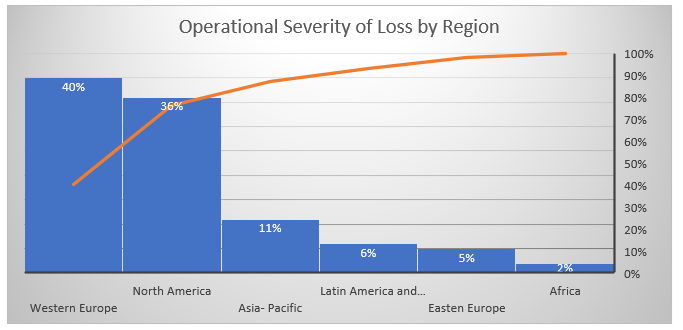
\includegraphics[width=1\linewidth]{ORX report Chat.png}
    \caption{Source: Annual Banking Loss Report ORX global banking database 2024}
    \label{fig:orx-report}
\end{figure}

The analysis in figure \ref{fig:orx-report} shows operational risk losses in the global banking system, revealing that Western Europe 40\% is the most affected region, followed by North America at 36\%. The majority 76\% of losses indicate higher exposure due to regulatory complexity, advanced automated financial systems, and high transaction volumes. Asia Pacific follows with a minimum risk profile of 11\%, as recorded above, and Latin America then accounts for only 6\%. Eastern Europe and Africa record the lowest \% rating, most probably due to underreporting and low banking activities. The cumulative trend shows that high losses are concentrated in developed nations and low-risk profiles in developing nations. 
\newpage
\textbf{Growth of the global banking operational loss database} (2014-2019)
\begin{table}[H]
    \centering
    \begin{tabular}{|c|c|c|c|}
        \hline
        Year & Total number of firms & Cumulative total gross loss (bn) & Cumulative frequency(OR Loss) \\
        \hline
        2014 & 80  & 247.00 & 419,954 \\
        2015 & 85  & 325.00 & 490,044 \\
        2016 & 92  & 371.00 & 566,590 \\
        2017 & 96  & 419.00 & 634,512 \\
        2018 & 97  & 458.00 & 695,139 \\
        2019 & 100 & 482.00 & 778,639 \\
        \hline
    \end{tabular}
    \caption{Summary of Firms, Gross Loss, and Operational Risk Events (2014-2019)}
    \label{tab:summary_table}
\end{table}
The Table \ref{tab:summary_table} was extracted from the ORX 2019 annual report database. From the findings, the participants observed an alarming rate of annual losses attributed to operational risk. As an association, ORX was established by a group of banks to create a global platform for secure and anonymous data exchange. This platform was established to help organisation evaluate their risk profiles and suggest the best possible ways to mitigate and reduce operational risk losses. 

The data in table \ref{tab:summary_table} indicate that cumulative total gross losses rose from \$247 billion in 2014 to \$482 billion in 2019, a nearly 95\% increase over five years. The frequency of operational risk events doubled from approximately 420 thousand events in 2014 to 780 thousand events in 2019. These figures indicate that overall exposure to operational risk is significantly increasing. Banks are facing double losses and higher risk events during this period. The number of firms participating increased from 80 to 100, accounting for a 25\% total increase. This suggests that a wider range of institutions is facing operational risk, contributing to the overall rise in global losses. The increase in both loss amounts recorded and frequency of events indicates that, without effective risk controls, the likelihood of getting high-severity losses will continue to rise.

\textbf{Basel Event Types: ORX Reference Taxonomy}
\begin{figure}[H]
    \centering
    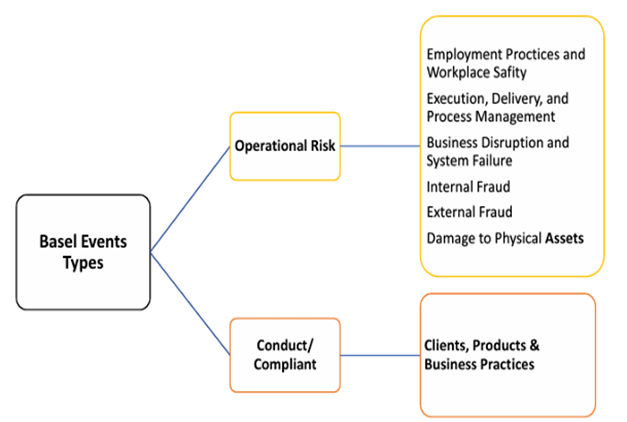
\includegraphics[width=1\linewidth]{Basel Event Types.png}
    \caption{Basel Event Types}
    \label{fig: Basel Event Types}
\end{figure}\\

The figure \ref{fig: Basel Event Types} illustrates the results of Basel Types and an analysis of the ORX Reference Taxonomy level 1s. This presents an essential framework for categorizing operational risk events in the banking and Insurance sector. The event types shown above were introduced under the Basel II framework and classify key risk events into seven broad categories: Internal Fraud, External Fraud, Employment Practices, Clients \& Products, Physical Assets, System Failures, and Process Management. Grouping and categorizing risk events help financial institutions to analyze loss events and implement effective policies to manage operational risk losses. ORX report refines these categories to reflect the evolving risk landscapes, such as cyber risk, third-party risk, and data management. They also break down the conduct and compliance risks into more specific components like financial crime and regulatory compliance. The comparison highlights how ORX's taxonomy simplifies the nature of operational risks, helping firms manage operational risk more effectively in today’s rapidly changing environment.

The rapid expansion of mobile money transfer platforms, digital banking, and Internet banking has led to a rise in operational risk, particularly in developing nations with poor security protocols and outdated banking systems in most companies. Several firms in Zimbabwe are affected by cyberattacks and data breaches every year. Econet Wireless was reportedly hit by a ‘Data Breach’, the suspect threatens to sell Econet's Customer database with 852,791 details of the customers, said the source, ZimDaily News (2025). Another similar incident occurred in 2024 when ZB Financial Holdings, one of Zimbabwe’s largest financial institutions, suffered a ransomware attack in July, resulting in a significant data leak.

Despite repeated attempts to contact ZB for comments, the company has not provided an official response, said the source, TechZim. National Foods lost over \$6 million to cybercriminals who hacked its systems and used phishing emails to deceive the finance manager into transferring funds. The scam involved two foreign suspects posing as a South African financial institution. According to Herald Zimbabwe (2017), Ok Zimbabwe lost 70,000 USD after one of its employees hacked into OK’s Money Wave system and made a transfer into his account. State-owned telecom company Netone claims it lost more than USD 1 million in potential revenue due to alleged fraud by one of its dealers, accused of illegally activating mobile lines without authorization in 2022, said the source, Kukurigo 2025.  According to Statista's report, the global cost of cybercrime is expected to surge in the next four years, rising from \$9.22 trillion in 2024 to \$13.82 trillion by 2028.

This research is essential due to the growing, alarming threat of operational risk in banks, insurance industries, and non-financial institutions. The integration of digital banking, mobile money transactions, and internet-based financial services paved the way for operational risk to those institutions with weak security protocols \parencite{cybersecurity2024}. As we can see from recent cyberattacks, data breaches, and fraud cases affecting major institutions in Zimbabwe, it is clear that many organizations are highly vulnerable. \textcite{madzudzo2021cybersecurity} asserts that global cybercrime costs are expected to increase significantly. 

Understanding the nature of risk is crucial for maintaining financial stability, ensuring regulatory compliance, and fostering consumer trust. To effectively manage these financial threats, organizations must quantify key risk indicators, enabling them to measure and mitigate potential financial losses that could disrupt business operations. A case study conducted by \textcite{ey2025operationalrisk} suggested that by establishing a robust framework to quantify operational risk, organizations across various industries will be better equipped to allocate resources effectively and implement targeted risk mitigation strategies, ultimately reducing potential losses. 

Operational risk is one of the most difficult risks to model. The challenges faced may include quantifying and validating Bayesian network models of operational risk for internal or external reviewers \parencite{zhang2023bayesian}. This research sets out a framework that I believe some other risk professionals may consider when quantifying and validating such models, concerning quantification of the network, probability eliciting, Protocols and bias, Validations of estimates, Structural model building, Risk process mapping and node identification, network structure, conditional probabilities and nodes discretion tables and Model structure validation. Bayesian networks are built upon a causal factor framework, pulling together the known (factors) and unknown (probabilities) into a visual node map to describe each risk process \parencite{ifoa2023operationalrisk}. The factors will be a mixture of firm-specific and external risk drivers.

It has been suggested that under the Basel II Accord, commercial banks have been required to calculate the operational risk capital charges, \parencite{shevchenko2013loss}. The Loss Distribution Approach is one of the suggested standard approaches used to quantify and validate the operational risk and capital charge. The fundamental issue in studying operational risk is the lack of a universal understanding of the actual meaning of operational risk among scholars, theorists, practitioners, and researchers. For this study, we use the definition proposed by the RBZ, and the one adopted in the Accord is “the risk of direct or indirect loss resulting from inadequate or failed internal processes, people, and systems or from external events, and this definition includes legal risk”.  It should be noted that according to this accord, this definition was developed for all financial institutions, Banks, and insurance companies concerning specific risk elements. According to the revised Basel Committee report, “legal risk includes but is not limited to exposure to fines, penalties, or punitive damages resulting from supervisory actions, as well as private settlements. 

How to construct a Bayesian Network diagram that establishes a relationship between the necessary operational risk attributes is not yet fully resolved. According to \textcite{basel2021principles}, and \textcite{difrancesco2023bayesian}, financial institutions must develop, implement, and maintain an operational risk management framework fully integrated into the institution’s overall risk management processes. Therefore, we need to clarify to what extent the quantifying methodologies allow the construction and validation of a model that considers the main features of all operational risks. The Basel Committee on Banking Supervision reviewed the operational risk management framework adopted by an individual institution and stated that a bank will depend on a variety of factors, including the nature, size, complexity, and risk profile of the bank. The losses generated by the operational risk are identified and connected under the international standards for the seven-event types, internal fraud, external fraud, employment practices and the safety of the working place, the clients, the products, and the commercial practices; the tangible assets loss, the activity rupture and the inadequate systems functioning and the process execution, the delivery, and management. 

This study aims to find better ways to understand and manage key risk indicators that are being faced in the financial sector industry. Using the Bayesian Network modeling, to create a visual map showing how different operational risk factors are connected and how they influence each other. This study also aims to figure out which factors are the most important in causing problems and how changes in one factor might affect other factors. This makes it easier for organizations to predict potential risks and take action to reduce them before they become bigger issues. Essentially, it's about building a smart Bayesian system that helps identify, measure, and validate the key causes of risks, leading to more effective and proactive risk management. Bayesian Networks can be effectively machine-learned from an operational risk incident database, enabling a risk manager to measure and report operational risk effectively and giving them the ability to manage and make informed decisions.

Several Authors have extensively explored the process and loss event analysis using the Bayesian Network modeling approach to better analyze and understand operational risk related to specific processes or sub-risk areas. Therefore, further research is needed to elaborate on how the Bayesian Network models can be constructed and learned, and then be applied in the effective management of operational risk at a bank or at an insurance company. How can these models be used in risk management and not just for regulatory reporting or risk calculation purposes? Also, how the models can allow for risk management to be viewed at a bank-wide or bank-unit-wide level and not just specific to a process or sub-risk type.

\section{Statement of the problem}

Operational risk is significant in all financial institutions, and it’s a major critical concern for financial institutions, as it can lead to substantial losses resulting from failures in internal processes or external events. Operational risk is hard to quantify, given the presence of heavy-tailed loss distribution \parencite{johanna2022capital}, and the lack of data usually for low-frequency and high-impact losses  \parencite{article}.  Despite regulatory advancements, such as the Basel II and Basel III Accords, operational risk modeling remains challenging due to the complexities in identifying, quantifying, and validating the interconnected causal relationships between risk factors. While traditional methods like the Loss Distribution Approach (LDA) are widely used, they do not fully quantify the key operational risk factors. 

Amongst the more sophisticated methods developed are linear models such as time series, econometric, and empirical actuarial models. These models rely on historical data to predict future values based on past trends. According to \textcite{dutta2006tale}, operational Risk losses often exhibit fat-tailed distributions, which means extreme losses would occur more frequently than would be predicted by linear models. Therefore, the relationship between variables in operational risks is non-linear and complex, making it difficult to model accurately using linear models. However, despite extensive research on operational risk, evidence for quantifying and validating key operational risk factors remains unclear.

Bayesian Network (BN) modeling presents a promising framework for addressing this gap by providing a probabilistic, causal structure that links risk factors in a visual node map. BNs allow for overcoming these hurdles as they combine qualitative data from experts and relevant quantitative data. Even with advances in modeling, challenges remain when it comes to building and validating these risk frameworks. It’s not always easy to define how different risk factors are connected, estimate the likelihood of certain events, or ensure that the model works in real-world scenarios. For many financial institutions, integrating these models into daily risk management, not just for ticking regulatory boxes, can be difficult because of how complex and technical they can be.

This study addresses the problem of developing the Bayesian Network framework for operational risk management, mainly focused on quantifying and validating causal relationships among key risk factors. The model seeks to enhance the understanding of how these models can be practically applied, enabling financial institutions to not only meet regulatory requirements but also improve proactive risk management at both the bank-wide and unit-specific levels.

\section{Aims and Objectives}
The primary aim of the study is to develop a framework using Bayesian Network (BN) modeling to identify, quantify, and measure operational risk in several business lines of commercial banking. The objective is to help risk professionals quantify and validate causal relationships between different operational risk factors. Therefore, by doing so, the study seeks to improve the accuracy and effectiveness of risk measurement and management practices.
\section{Main Objectives}
These objectives aim to establish a comprehensive framework for modeling operational risk using Bayesian Networks, allowing for the quantification, validation, and interpretation of causal relationships between risk factors.
 \subsection{Primary Objectives}
These objectives aim to establish a comprehensive framework for modeling operational risk using Bayesian Networks, allowing for quantifying, validating, and interpreting causal relationships between risk factors.
\begin{enumerate}
    \item Construct a Bayesian Network (BN) Framework: To develop a BN diagram that accurately establishes relationships between the key operational risk attributes, illustrating how different factors influence each other.
    \item Quantify the Network and Validate Estimates; To quantify the network by estimating probabilities associated with different risk scenarios and events
    \item Validate the Model Structure; To validate the Bayesian Network model structure, ensuring that it accurately represents the causal relationships and can be used for effective risk management.
\end{enumerate}

\subsection{Research questions}
To manage operational risk effectively, the factors thought to influence the key risk factors should be identified and addressed. Ideally, the research questions are designed to explore major aspects of using Bayesian Networks for operational risk modeling, from constructing the framework to validating its structure and probability estimates. 

\begin{enumerate}
    \item How can the Bayesian Network (BN) diagram, which represents the relationships between key operational risk attributes, be constructed effectively?
    \item What are the critical steps to quantify the dependency between risks, and which methods can be used to quantify the network and accurately estimate the probabilities associated with various operational risk factors?
    \item What are the critical steps for mapping the risk process and identifying key nodes within the Bayesian Network structure for operational risk modeling?
    \item What role do conditional probability tables and nodes' discretion play in defining the relationships within a Bayesian Network for operational risk?
    \item What are the challenges in using Bayesian Networks for operational risk modeling, and how can they be addressed through model validation and structural refinement?
\end{enumerate}

\section{Justification/Rationale or Significance of Research}
The research will be of significance to different stakeholders as follows: 

\subsection{To Banks and other organizations: }
Banks will be able to measure and quantify the key operational risk and approximately estimate the capital charge that might be required in case of severe risk occurring, and also to measure the level of risk awareness within the organization.  To other organizations, the research will represent a proxy of guidance for their operational risk management programs. The study is significant to both stakeholders and education 5.0, as the following shows the importance of choosing the Bayesian Method as a tool used to assess the impact of operational risk.

According to Yew (2020), the graphical presentation of BNs aids the understanding of the causal structure. It presents the risk profile of the company intuitively, improving management's knowledge of, and hence participation in, the management of operational risk.  This study provides a robust framework for modeling and managing operational risks, allowing organizations to better understand and mitigate risks, leading to more informed decision-making.

Traditional linear models may struggle to capture the complex, non-linear dependencies often found in operational risk scenarios. Conditional probabilities can be quantified to take into account the impact of controls and mitigating actions, thus providing a platform for what-if analysis, helping to analyze the effect of specific controls and identifying which controls have the most impact on resultant loss, which can be used in future planning and investment choices Therefore, using the Bayesian Networks helps overcome these limitations, providing a more flexible and sophisticated approach to modeling risk factors and their interactions.

Operational risk losses often have "fat-tailed" distributions, meaning that extreme losses occur more frequently than expected under standard models. The proposed Bayesian Network framework can better accommodate and model these extreme events, offering a more realistic assessment of risk.

Financial institutions face regulatory requirements for quantifying and managing operational risk. This study's framework can help firms meet regulatory standards by providing a validated model for risk quantification, which is essential for calculating capital reserves and demonstrating compliance with industry guidelines \parencite{IMF2023_Zimbabwe}.

Bayesian decision networks provide a cost-benefit analysis of risk controls, where the optimal controls are determined within a scenario analysis framework. The Bayesian Network approach allows for stress testing and scenario analysis, enabling organizations to test how the models perform under different conditions.  Scenario building is identifying the critical factors that contribute to an adverse event and crafting a narrative that briefly describes the circumstances and consequences if it were to happen. This will help to identify whether the Bayesian Network can effectively capture the impact of catastrophic events or emerging risks.
\subsection{To the Researcher}
The researcher will gain valuable insights from a different angle of risk management to augment his valuable banking experience and hopes to expand and broaden his knowledge. The academic world will benefit from the valuable, diverse literature as applied in a real organization
\subsection{Practical Implications for Operational Risk Managers:}
The framework provides operational risk managers with practical tools for mapping risk processes, identifying key risk factors, and validating risk models. One of the key advantages of Bayesian Network models is that they can easily be visualized with the use of the node or factor map \parencite{article}. These visuals are easy to understand for any stakeholder in the business, allowing a broader range of stakeholder challenges. It is widely accepted that this will enhance the understanding of each business process and its associated risks and controls, providing a closer link between risk measurement and risk management approaches.

One of the advantages of using a Bayesian network as a modeling tool is that it can answer queries that are both predictive and diagnostic \parencite{sanford_bayesian_2012}. For example, a predictive query may ask, “What is the probability of a payment failure given that a loan is being processed?”, whilst a diagnostic query may ask, “What is the most probable transaction type processed given that a payment failure occurred?”. Experts agree that, having observed the state of an effect node, such as a payment failure, inference can be carried out to show the probable states of the causal nodes within the network modeling in structured finance operations. 

The Bayesian Network provides an effective technique for quantifying and modeling operational risk \parencite{zhao_data_2024}. The model can be utilized across several areas of study, including areas such as improving operational continuity, evaluating response strategies, and assessing newer risks like those related to cybersecurity and climate change. In addition, the Bayesian Framework allows better strategic decisions, as it enables the assessment of various management responses under different operational risk conditions.
 
\subsection{Assumptions for Learning the Causal Structure}
The Causal Sufficiency Assumption and the Markov Assumption are foundational theories for applying Bayesian Networks (BNs) practically. According to \textcite{Chobtham2020}, and \textcite{Wu2023}, the Causal Sufficiency Assumption states that no unobserved variables act as common causes of two or more observed variables within the domain. This assumption is critical for ensuring that observed dependencies and independencies in the data accurately reflect the true causal structure rather than omitted confounders.

The Markov Assumption, integral to the BN framework, asserts that a variable is conditionally independent of its non-descendants given its parents and this property enables the factorization of the joint probability distribution into conditional probabilities, facilitating efficient computation and inference. When the Causal Sufficiency Assumption is violated, the Markov property may fail, as unobserved variables introduce dependencies not accounted for in the model. Such violations can be seen as unexpected conditional dependencies in the data, undermining the reliability of the BN’s conclusions about causal or probabilistic relationships.

To address the challenges posed by latent variables, methodological advancements have focused on techniques such as instrumental variables (IVs), which exploit exogenous variation to estimate causal effects in the presence of unobserved confounding. Ongoing research extends these principles to develop tests for detecting latent variables in constrained settings and to enhance BN frameworks through hybrid models, such as structural equation models (SEMs), which explicitly incorporate latent variables. These approaches aim to reconcile the theoretical precision of BNs with the complexities of real-world data, where unobserved variables are pervasive.

The Causal Sufficiency and Markov Assumptions provide a powerful framework for modeling probabilistic and causal relationships; their real-world applicability is assumed to be effective in real-world data as according to  \textcite{Fazio2024}, \textcite{Asgari2024}, and \textcite{Miklin2021}. Acknowledging these limitations underscores the importance of integrating complementary methods—such as IVs, latent variable modeling, or hybrid SEMs—to enhance the robustness of BN-based analyses.

\subsection{Scope of Research/Delimitation of the Study}
Operational risk has become the major trending topic in financial institutions, but from all the findings available, there is no significant research that has been done to quantify and characterize operational risk. There are limited studies on operational risk management, and most studies have tended to focus on traditional methods to model operational risk in financial services organizations. 

Developing a Bayesian modeling framework is the underlying theme of this study, and this study will provide a robust framework for managing operational risks, allowing organizations to better understand and mitigate risks, leading to more informed decision-making. Research suggests that BN framework can be structured in such a way to have the various operational risk factors cascade into an overall loss, thus allowing risk capital to be specified. The built-in causal relationships within Bayesian Networks make them effective tools for detecting and assessing the consequences of operational loss incidents. This aligns with the key criteria expected of operational risk models in the financial sector.

\section{Definition of Key Terms}
\subsection{Bayesian Network}
Bayesian networks are directed acyclic graphs that allow efficient and effective representation of the joint probability distribution over a set of random variables \parencite{sanford_operational_2015}. In this graphical structure, nodes correspond to random variables, while edges illustrate direct relationships between them. The network captures conditional independencies by ensuring that each variable is independent of its non-descendant variables, provided the values of its parent nodes are known. \textcite{unknown} and Atakan (2019) defined the Bayesian Network as a Probabilistic Graphical Model (PGM) that represents conditional dependencies between random variables through a Direct Acyclic Graph (DAC), which can be applied in many fields, particularly for operational risk in financial institutions. 
\subsection{Operational Risk}
Operational risk (OR) is defined by the Basel Committee on Banking Supervision (BCBS) as the risk of loss resulting from “inadequate or failed internal processes, people and systems or from external events”. It is a fundamental element of risk management at banks \parencite{bcbs2004basel2}. The actual definition of operational risk presented by the Basel II becomes the international standard definition recognized. This ascertains that Operation risk can be classified as the uncertainties and potential hazards a company faces while conducting its day-to-day business operations. Unlike systematic risk, which stems from external forces such as economic or political events, operational risk is primarily linked to an organization's internal operations, decision-making processes and internal system failures.
\subsection{Quantification of operational risk }
Quantification of operational risk can be described as the process of measuring losses and assessing the potential losses from the identified key risk indicators, Internal Failures, Human errors, System Failures, Disasters, and external business disruptions \parencite{kim2021system}. This process involves the use of probability elicitation and probability graphical models to represent and analyze the dependencies between various risk factors and events. This method uses combined historical data, expert judgment for probability elicitation, and scenario analysis to update risk probabilities as new data becomes available. This effectively ensures more accurate risk assessment and mitigation strategies.
\subsection{Scenario Analysis}
According to \textcite{fenton2010managing}, Bayesian decision networks provide a cost-benefit analysis of risk controls, where the optimal controls are determined within a scenario analysis framework. The Bayesian Network approach allows for stress testing and scenario analysis, enabling organizations to test how the models perform under different conditions \parencite{rippel_operational_2011}. Scenario development involves pinpointing key elements that could lead to a negative event and constructing a concise description outlining the context and potential outcomes should the event occur. This will help to identify whether the Bayesian Network can effectively capture the impact of catastrophic events or emerging risks.
\subsection{Casual Analysis}
Scholars have suggested that causal analysis is an effective way to understand what causes operational losses in the business environment. Causal analysis, just like scenario analysis, looks at the historical losses and updates the likelihood of different risk factors being responsible \parencite{andersen2016causal}. Causal analysis analyzes in a better way, rather than predicting losses, diving much deeper into the causes and interrelationships between variables. Taking this into consideration, if a Bank is facing losses and wants to prevent further losses, it needs to identify the main causes of the major losses.  Through a deep analysis, the bank can easily find out which risk factors are causing the losses, Maybe, data quality, weak security protocols, and system failure have the biggest impact. This plays a crucial role in helping companies improve their systems and reduce risks more effectively. 
\subsection{Loss Distribution Approach}
The Loss Distribution Approach is a statistical technique that estimates the distribution of losses based on historical data \parencite{wang_method_2017}. \textcite{hadley_selection_2019} argues that LDA assumes that operational losses are driven by two independent factors, which are as follows: the frequency and the severity of the event. The frequency is the number of loss events that occur in a given period, such as a year. The LDA works like this: we list out all the things that could go wrong for a company, such as Fraud, system glitches, execution errors, and legal issues. Then, we figure out how likely each event is and how much money it will cost. then create a sort of overall Bayesian map showing the possible losses and decide how much money it needs to have on hand (Kind of like a safety net) to cover unexpected financial loss from the potential issues.
\newpage
\textbf{Overview of the this research analysis}
\begin{itemize}
    \item \textbf{Chapter 1 - Introduction} - This chapter provides an overview of the study, covering the aims, objectives, statement of the problem, significance of the study, delimitation, and limitations.
    
    \item \textbf{Chapter 2 - Literature Review} - This section examines the literature relevant to related studies and theoretical background.
    
    \item \textbf{Chapter 3 - Methodology} - This chapter describes the research methodology, including analytical tools and procedures used to conduct the study.
    
    \item \textbf{Chapter 4 - Data Analysis \& Results} - This section presents the analysis of data and interpretation of the results.
    
    \item \textbf{Chapter 5 - Conclusion, Discussion, Recommendations, and Limitations} - The final chapter covers the summary, conclusions, and recommendations derived from the data analysis and interpretation of results.
\end{itemize}
\newpage
\section{Chapter Summary}
This chapter serves as an introduction to this project on operational risk modeling within financial institutions, emphasizing the challenges associated with accurately identifying, quantifying, and validating key risk factors. The chapter discussed the Background of the Study, highlighting the impact of operational risk losses, limitations of traditional modeling methods, and the potential of Bayesian Network (BN) modeling to address these challenges by mapping complex causal relationships among risk factors. 

The Problem Statement addresses the need for a robust framework that goes beyond regulatory compliance, aiming to support proactive risk management through the integration of BN models. The Objectives and Aim of the Study outline the goals of developing and validating a Bayesian framework for quantifying and understanding operational risk factors and enhancing its practical application for financial institutions. The Delimitation of the Study defines the scope, focusing on key operational risk factors within the context of a Bayesian Network structure. Lastly, the Layout of the research provides an overview of the research structure.

The next chapter to follow is going to discuss the relevant literature and theoretical frameworks related to operational risk and Bayesian Network modeling.



\chapter{LITERATURE REVIEW}
\section{Introduction}
A literature review is a critical synthesis of existing research and scholarly resources relevant to a specific field of study, as suggested by \parencite{walker2010systematic}. In the context of Bayesian Network modeling for operational risk, this literature review will explore published academic articles and journals, industry guidelines, and other relevant resources that address the framework for quantifying and validating causal relationships in operational risk management. By examining prior research on using Bayesian Networks to model operational risk and establish a framework for quantifying and validating causal relationships, this chapter aims to highlight the current state of knowledge and identify gaps that the present study seeks to address. The literature review will objectively summarize past studies, methodologies, and findings while critically assessing their contributions to the field. This will help establish a theoretical foundation for the study and clarify the rationale for employing Bayesian Network modeling to improve operational risk management practices. Through this process, the chapter will demonstrate how integrating causal modeling can enhance the framework's effectiveness for quantifying and validating causal relationships in operational risk management.
\subsection{Operational Risk}
Operational risk has emerged as a major focus within the financial sector, largely because of its influence on the routine functioning of economic institutions. This growing interest has drawn the attention of industry professionals, regulators, and academics alike. Studies have shown that a key challenge in this field remains the absence of a commonly accepted definition of operational risk across different expert communities. For this study, we use the definition proposed by the \textcite{bcbs2020operationalrisk}, and the one adopted in the Accord is” the risk of direct or indirect loss resulting from inadequate or failed internal processes, people and systems or from external events, and this definition includes legal risk”.  It should be noted that according to this accord, this definition was developed for all financial institutions, Banks, and insurance companies concerning specific risk elements. According to the revised Basel Committee report, “legal risk includes but is not limited to, exposure to fines, penalties, or punitive damages resulting from supervisory actions, as well as private settlements.

The table \ref{tab:risks} in the next page outlines a structured Operational Risk Taxonomy, categorizing risks into Level 1 (broad categories) and Level 2 (detailed sub-risks). It covers people, fraud, technology, process failures, and conduct. This classification helps firms systematically identify, assess, and manage operational risks, ensuring compliance with regulatory standards like Basel and enhancing risk control and reporting.

\begin{table}[H]
\centering
\caption{Level 1 and Level 2 Operational Risks}
\label{tab:risks}
\resizebox{\textwidth}{!}{%
\begin{tabular}{|l|l|}
\hline
\textbf{Level 1 Risks} & \textbf{Level 2 Risks} \\
\hline
\multirow{4}{*}{People} 
 & Breach of employment legislation \\
 & Breach of regulatory requirements \\
 & Ineffective employment relations \\
\hline
\multirow{3}{*}{External Fraud} 
 & Third party/vendor fraud \\
 & Agent/ Broker/ Intermediary fraud \\
 & First party Fraud \\
\hline
\multirow{3}{*}{Internal Fraud} 
 & Internal fraud committed against the organisation \\
 & Internal Fraud committed against Customer \\
 & Internal Fraud committed against Clients \\
\hline
\multirow{3}{*}{Physical Security and Safety} 
 & Damage to the organisation's physical properties \\
 & Injury to employees/affiliates outside the workplace \\
 & Damage to or injury to public assets \\
\hline
Business Continuity 
 & Inadequate business continuity planning or event management \\
\hline
\multirow{5}{*}{Transaction or Processing and Execution} 
 & Execution failure relating to clients and products \\
 & Execution failure relating to securities and collateral \\
 & Execution failure relating to the third party \\
 & Execution failure relating to internal operations \\
 & Change execution failure \\
\hline
\multirow{3}{*}{Technology} 
 & Hardware failure \\
 & Software failure \\
 & Network failure \\
\hline
\multirow{12}{*}{Conduct} 
 & Insider trading \\
 & Improper market practices \\
 & Post service failure \\
 & Client Mistreatment \\
 & Client Account Mismanagement \\
 & Improper distribution/ marketing \\
 & Improper product or service design \\
 & Breach of code of conduct \\
 & Employee misbehaviour \\
\hline
\end{tabular}%
}
\end{table}

\subsection{An interconnected operational risk landscape }
An increasing interconnectivity of the operational risk landscape is rapidly changing the way risks are viewed and assessed. The recently published report by ORX shows that among actively participating members, emerging operational risks are fully interconnected, where the boundaries between individual risk and associated internal and external risk factors cannot be easily separated. The Bayesian Belief Network presents a promising way to tackle this through the use of a direct cyclic graph, a local Markov property, to assess and drive a better understanding and visibility of vulnerabilities, interconnections, and concentrations of risk (often undertaken as part of operational resilience efforts). The interconnectedness between individual risks creates a combined risk profile that exceeds the sum of its parts. The report shows that in the context of geopolitical uncertainty and economic strain, it is surprising that cybercrime ranks as the top emerging risk.

The Reserve Bank of Zimbabwe (RBZ), Financial Stability reports produced from 2022 to 2024 agree with the ORX global report that cybercrime is ranked as the highest risk indicator. The integration and adoption of more sophisticated AI machines, business software, and do-it-yourself portals have significantly increased the cases of cyberattacks in many companies as they are exposed to the risks associated with rapid technology advancement. Organizations must take this opportunity of rapid growth in technology to harness these innovations, which help in managing risks from outdated banking systems amongst other related automated systems. Concerns about risks from outdated machines, systems, and increased business disruptions are amplified by heavy reliance on a complex network of third-party providers, particularly concentrated around cloud service providers, creating potential systemic risks. At the same time, regulatory pressures are intensifying the focus on these critical areas.
\subsection{Operational Risk surfaces expand as a trade-off to rapid digitalization}
Businesses must digitalize not only to seize new opportunities but also to stay competitive. The speed of change requires institutions to carefully balance the risks of hurried change management, accumulating technical debt, outdated legacy systems, and security issues introduced by new technologies against the risk of falling behind. The rapid pace of technology transformation from old systems to AI and automated systems is also complicating the cost-benefit analysis related to the control environment. Ultimately, this ongoing transformation increases the exposure of institutions to risks in ways that are difficult to predict and evaluate. In a rapidly changing risk environment, Bayesian networks allow firms to understand how different risks influence each other, quantify the probability of cascading failures, and update risk assessments as new information emerges. This dynamic modeling helps businesses anticipate potential vulnerabilities across their digital transformation, operational processes, and third-party dependencies, enabling proactive risk management.
\begin{figure}[H]
    \centering
    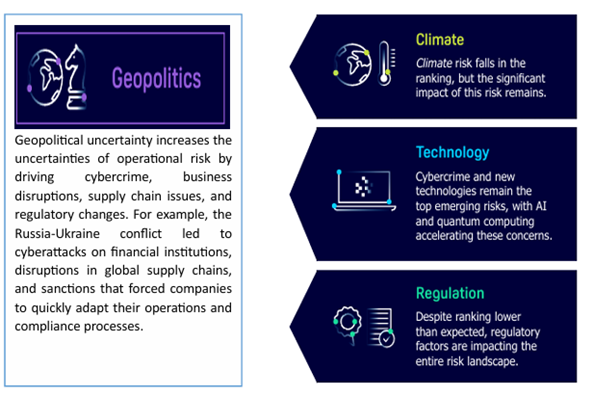
\includegraphics[width=0.75\linewidth]{External Environment.png}
    \caption{A rapidly evolving external environment }
    \label{fig: External environment}
\end{figure}
Figure \ref{fig: External environment} describes various factors contributing to operational risk, including geopolitical uncertainty, climate change, technological advancements, and regulatory shifts. Geopolitical instability, such as the Russia- Ukraine conflict, heightens cyber threats, disrupts supply chains, and forces businesses to adapt to evolving regulations. While climate risks have declined in ranking, their impact remains significant. Emerging technologies, particularly AI and quantum computing, continue to escalate cyber risks, whereas regulatory changes affect the broader risk landscape. Together, these factors increase operational risk complexity, necessitating proactive risk management strategies for business resilience.
\subsection{Percentage of global total loss falling in each loss size bin}
\begin{figure}[H]
    \centering
    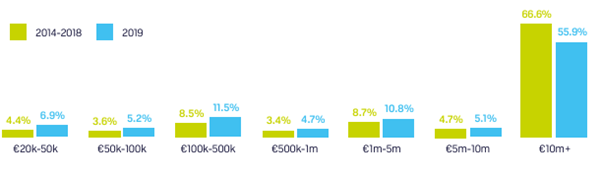
\includegraphics[width=1\linewidth]{Global Total Loss 1.png}
    \caption{The distribution of total monetary losses }
    \label{fig: Total monetary losses}
\end{figure}

\begin{figure}[H]
    \centering
    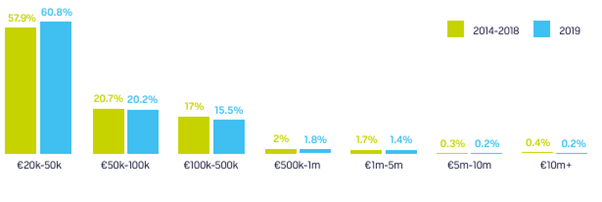
\includegraphics[width=1\linewidth]{Global Total Loss 2.png}
    \caption{The total percentage of the number of events }
    \label{fig: Percentages}
\end{figure}
Figure \ref{fig: Total monetary losses} illustrates the distribution of total monetary losses across various loss-size categories. The data shows that high-value loss events exceedingly more than USD 10 million account for the largest share of overall loss, often exceeding 50\% of the total. In contrast, smaller loss bins (e.g., below \$50,000.00) represent a relatively minor portion of total losses. This suggests that while smaller events may occur frequently, a few very large incidents drive the majority of the financial impact.

Figure \ref{fig: Percentages} above focuses on the percentage of the number of events occurring in each loss-size category. Unlike Figure \ref{fig: Total monetary losses}, it reveals that the majority of incidents fall into smaller loss bins (for instance, under \$20,000.00 or between \$20,000.00 and \$50,000.00). Large-scale risk events above 10 million remain relatively rare., This typically constitutes a small fraction of the total events. This discrepancy between Figures 7 and 8 underscores a key operational risk insight: Most loss incidents are relatively minor, but a small number of severe events account for the greatest financial impact.

The ORX data indicates a growing trend in cumulative losses and a growing number of operational risk events, with high-severity incidents driving most of the total financial impact \parencite{orx2024lossdata}. Meanwhile, smaller losses are much more frequent, yet represent a smaller portion of the aggregate loss. This pattern highlights the need for robust modeling techniques that can capture both frequent low-level incidents and rare but high-impact events. In the literature, Bayesian Belief Networks (BBNs) have gained attention as a powerful tool for quantifying operational risk, as they allow the integration of empirical data and expert judgment to model dependencies among risk factors, estimate the probability of extreme events, and ultimately support more effective risk mitigation strategies.

How to construct a Bayesian Network diagram that establishes a relationship between the necessary operational risk attributes is not yet fully resolved. As previously stated in \textcite{basel2021principles}, Banks must develop, implement, and maintain an operational risk management framework that is fully integrated into the institution’s overall risk management processes. Therefore, we need to clarify to what extent the quantifying methodologies permit the construction and validation of a model that considers the main features of all operational risks. The Basel Committee on Banking Supervision reviewed the Operational risk management framework adopted by an individual institution and stated that a Bank will depend on a range of factors, including the bank’s nature, size, complexity, and risk profile. The losses generated by the operational risk are identified and connected under the international standards for the seven-event types, internal fraud, external fraud, employment practices and the safety of the working place, the clients, the products, and the commercial practices; the tangible assets loss, the activity rupture and the inadequate systems functioning and the process execution, the delivery, and management  (Barbu et al, 2010). 

\section{Empirical Literature}
\subsection{Bayesian Network Structure and Operational Risk }

The quantification of operational risk under the regulatory standards Basel II and Solvency II is a challenging task; many financial institutions adopt a Loss Distribution Approach to estimate this risk capital charge (Klugman, Panjer and Willmot, 2008), Operational Value-at-Risk,\textcite{sanford_operational_2015}, and Scenario analysis Approach, \textcite{andersen2016causal}. These approaches require a combination of internal and external data, as well as expert opinions. The Bayesian Network scenario to estimate the parameters of the risk frequency and severity distributions has been proposed by \parencite{aquaro_bayesian_2009}, to provide insights into the estimation of operational risk.

Bayesian network structure can be defined as a probabilistic graphical model that explicitly captures the known conditional dependence with directed edges in a graph model \parencite{janson2019bayesian}, with all the missing connections defining the conditional independencies in the model. \textcite{ramamurthy2005operational} described the Bayesian Network as a quantitative or causal probabilistic network that helps, model, measure, and manage operational risk before knowledge of the causal risk factors and probabilistic reasoning. Bayesian Networks provide a useful tool to visualize the probabilistic model for a domain, review all of the relationships between the random variables, and reason about causal probabilities for scenarios given available evidence. According to Janson, Bayesian network models capture both conditionally dependent and conditionally independent relationships between random variables. 

\textcite{guney2019introduction}, defined the Bayesian Network, or Belief Network as a Probabilistic Graphical Model (PGM) that represents conditional dependencies between random variables through a Direct Acyclic Graph (DAC) which can be applied in many fields, particularly for this research we are mainly focused on the operational risks which are being faced in all financial institutions. More precisely, Bayesian networks are directed acyclic graphs that allow efficient and effective representation of the joint probability distribution over a set of random variables as alleged by \textcite{fenton2008using} and \textcite{leo2020managing}. Each vertex in the graph represents a random variable, edges represent direct correlations between the variables, and the network encodes the conditional independence statements where each variable is independent of its non-descendants in the graph given the state of its parents. These independencies are then exploited to reduce the number of parameters needed to characterize a probability distribution and to efficiently compute posterior probabilities. Probabilistic parameters are encoded in a set of tables, one for each variable, in the form of local conditional distributions of a variable given its parents. 

\textcite{pearl1988probabilistic} claims that the Bayesian Theory contains information about causal probability relationships between variables and is used for decision-making in managing risk. The causal probability relationships in a Bayesian Theorem are represented by nodes which depict the variables and direct arcs which represent the conditional relationship in the form of a direct acyclic graph. Bayesian Networks are suitable for modeling operational risk because they can represent complex causal relationships between risk factors and quantify uncertainties probabilistically. This theory supports the integration of expert knowledge and data, allowing for a comprehensive analysis even when data is scarce or incomplete \parencite{alexander2006bayesian}. BNs enable scenario analysis and inference by updating probabilities based on new evidence, which is essential for stress testing and dynamic risk assessment. More precisely, their structure facilitates model validation, as the causal dependencies can be compared with empirical data to ensure consistency and accuracy \parencite{cowell_modeling_2007}.

Financial databases usually constitute high noise and nonlinearity levels, making it difficult to train deep learning models like Deep Belief Networks, Bayesian Belief Networks, and Convolutional Neural Networks \parencite{liu_risk_2021}.

\textbf{High noise:}
\begin{equation}
x_i = x_i^{\text{true}} + \varepsilon_i, \quad \varepsilon_i \sim \mathcal{N}(0, \sigma^2)
\end{equation}
where \( \varepsilon_i \) represents Gaussian noise with high variance \( \sigma^2 \)] and \( \eta_i \) is additional noise.
\vspace{10pt}

\textbf{Nonlinearity:}
The underlying function \( f: \mathbb{R}^d \rightarrow \mathbb{R} \) relating \( x_i \) and \( y_i \) is highly nonlinear, i.e.,
\begin{equation}
y_i = f(x_i) + \eta_i
\end{equation}

Bayesian Belief Network models require substantial amounts of training data, but financial data offer a more complex, limited dataset, which makes it more challenging to validate the models. The application of advanced sophisticated financial risk models in the financial industry presents several advantages. BBN can handle large-scale high-dimensional data in both industries, the Health, Financial, and manufacturing industries as illustrated by \textcite{zhao_data_2024}, and unearth hidden patterns and trends, aiding in identifying potential risk factors and correlations. BBN models present strong generalisation capabilities that are adaptable to operational risk management needs across different types and domains (Yazdi et al., 2024). 

In addition, BBN and Deep Network analysis can automate risk identification and quantification, determining the minimum capital reserve for banks, and insurance industries \parencite{buddiga_advancing_2022}. The integration of artificial intelligence in operational risk management has increasingly led to rapid expansion of new perspectives and more advanced tools with powerful data processing and analytical capabilities across various industries. Amongst the newly adopted data analytical tools, is machine learning through AI, deep learning, and big data analytics Shi et al.(2025) and \textcite{feng2024deep}. These analytical tools offer a promising solution to the rapid advancement in technology towards risk management. The world is rapidly moving towards new tech, which concurrently comes with its potential limitations to the industry, as cyber attackers find loopholes in outdated banking systems, and phishing schemes become prominent in underdeveloped nations.

This literature presents the opinions of various authors regarding the Bayesian Network analysis of operational risk.\textcite{hager_knowledge_2010}, suggested the Bayesian Network as a powerful tool for quantitative analysis of the causal relationships determining the loss severity. This framework has been suggested to solve the problem of scarce data by data-driven models and also improving scenario-based methods. They constructed a causal model based on the mechanisms that determine the loss size for a specific event and further modeled the root causal drivers for the identified loss determinants. They found that the Bayesian model framework provides a formalized model structure and scientifically sound theoretical basis for scenario modeling.


\textcite{shevchenko2009implementing} applied the Loss distribution approach for operational risk, which allows to take into account expert judgment and parameter uncertainty into account, modeling dependency from their observations the Bayesian framework is convenient for combining different data sources (internal data, external data, and expert opinions) and to account for the relevant uncertainties. It has been noted that accurate quantification of the dependencies between ORs is a difficult task with many challenges to be resolved. Therefore, many aspects of the LDA may require further research. 

Therefore, a study carried out by \textcite{tudor_operational_2017} reviewed the usual ways of quantifying operational risk in Loss Distribution Approach (LDA) models. In their findings, they recommended that we clarify to what extent the quantifying methodologies permit the construction of a model that considers the main features of all operational risks in any financial institution.  A research study by \textcite{sanford_operational_2015} developed an operational risk modeling tool using a Bayesian network to capture causal relationships between risk factors and losses. The research provides a prediction of operational loss distributions and, and Operational Value for-risk management. Continuous variables were approximated using static discretization, though more sophisticated methods were used. From their findings, the Bayesian enhances risk prediction, adaptability, and communication in operational risk management. Another related research, by \textcite{liu_bayesian_2022} addressing the key aspect of operational risk shows that the Bayesian framework enables effective risk management. The research employs vine copulas within a Bayesian framework to model dependencies between different types of data breaches, whilst using public data sets, the study finds that the optimal vine structure provides more conservative value-at-risk estimates than other models. 

A case study conducted by \textcite{universidad_panamericana_operational_2017} focused on quantifying capital requirements for operational risk in a Mexican financial institution using an advanced Bayesian inference model has revealed that operational risk can be estimated with 95\% confidence even with limited data, with a positive correlation between expert expectations and operational risk levels. Their primary objective was to develop a robust operational risk measurement framework, in cases where historical loss data is insufficient. The study employs a conjugated Poisson-Gamma distribution, integrating expert interviews to estimate parameters, and utilizes Monte Carlo simulations to model expected losses. Furthermore, the frequency and severity of losses fluctuate dynamically as the risk threshold is approached. These insights highlight the importance of model assumptions and expert input in risk quantification. The proposed methodology serves as a foundation for developing risk mitigation strategies, enabling financial institutions to proactively manage operational risk and minimize potential losses.

Bayesian network models have been and continue to be applied to diverse problem domains, particularly in the financial sector industry. Other statisticians argue that operational risk managers are not interested in the characterization or categorization of operational risks, but rather in the frequency and severity of operational losses \parencite{hager2010knowledge}, which gives the number of monetary losses incurred. The research analyzed operational losses to understand their causes and impacts, using data warehouses for low-impact, high-frequency losses, and qualitative methods for rare, high-impact events. The key findings indicate that storing loss data and using Management information system reports helps identify key risk drivers, while qualitative approaches like self-assessments foster a culture of risk awareness. This approach is relevant to operational risk management as it supports decision-making by providing insights into frequent losses and focuses on qualitative strategies for rare risks.

The Bayesian Network can incorporate the elements of the Advanced Measurement approach, which include internal data, external data, scenario analysis, and factors reflecting the business environment and the control system in a simple. \textcite{martinez2016analysis} applied the Bayesian approach to manage Operational Risk in the international banking sector, incorporating real-world elements like specific risk distributions and expert opinions. As preferred by other scholars, Bayesian Networks offer advantages over other models by integrating internal and external data, scenario analysis, and causal relationships. They provide a more realistic framework for calculating operational risk, highlighting the Bayesian Network's effectiveness in Operational Risk management.

\textcite{tudor_operational_2017}, developed a Bayesian Network framework for quantifying and validating operational risk key factors, and in their findings, they picked some limitations in the current operational risk management. Their main findings depict a lack of rigorous backward-looking validation of forecasts and simulations. They advised that estimations used for risk quantification should be validated with econometric tests and that the actual outcomes should be compared to predict risks. Other Authors argue that the absence of detailed historical data on multiple causes affects the ability to perform thorough post-event analysis, making the simulation process a potential operational risk. Automation and technology, such as blockchain, could improve data collection and standardization, enabling better causal relationship analysis and risk quantification. To enhance Bayesian network models for operational risk, incorporating comprehensive data on causal relationships and using tools like process diagrams could help validate and quantify risks more effectively.

In addition to the above, operational risk is significant in all financial institutions and it’s a major critical concern for financial institutions, as it can lead to substantial losses resulting from failures in internal processes, or external events. Operational risk is hard to quantify, given the presence of heavy-tailed loss distribution (Martin et al, 2020), and the lack of data usually for low-frequency and high-impact losses (Acharyya et al, 2023).

Despite regulatory advancements, such as the Basel II and Basel III Accords, operational risk modeling remains challenging due to the complexities in identifying, quantifying, and validating the interconnected causal relationships between risk factors. While traditional methods like the Loss Distribution Approach (LDA) are widely used, they do not fully quantify the key operational risk factors. Amongst the more sophisticated methods developed are linear models such as time series, econometric, and empirical actuarial models. These models tend to rely on historical data to predict future values based on past trends.  Operational Risk losses often exhibit fat-tailed distributions, which means extreme losses would occur more frequently than would be predicted by linear models. Therefore, the relationship between variables in operational risks is non-linear and complex, making it difficult to model accurately using linear models. However, despite extensive research on operational risk, the significance for quantifying and validating key operational risk factors remains unclear. 

\textcite{zhao_data_2024} traditional risk management methods rely heavily on historical data and statistical models, and are no longer effective in the highly volatile and fast-changing financial sector. He developed a law risk prediction model called WBIF, which integrates Bidirectional Long Short-Term Memory (BiLSTM) and Fully Convolutional Networks (FCN), with parameter optimization performed using the Whale Optimization Algorithm (WOA). The study focused on improving the accuracy and adaptability of risk prediction in financial markets. The main findings show that the WBIF model reduced the Mean Absolute Error (MAE) by 51.73\% on the UCI machine learning dataset and improved accuracy by 12\% on the Kaggle credit card fraud detection dataset. The study concluded that deep learning models optimized with advanced algorithms like WOA can significantly enhance risk prediction accuracy, surpassing traditional statistical approaches.

A study carried out by \textcite{eze2024harnessing} asserts that operational risk management is crucial for organizations to protect themselves from disruptions, financial losses, and reputational harm. The author used a methodology that examined the role of data analytics in enhancing operational risk management to study how organizations can leverage advanced analytics techniques to manage risks more effectively. The main findings show that data analytics enables organizations to extract actionable insights from large data sets, allowing them to identify, assess, and mitigate risks proactively. The study ends by concluding that by integrating data analytics into operational risk management, organizations can strengthen their operational resilience and enhance long-term business sustainability.

Bayesian Network (BN) modeling presents a promising framework for addressing this gap by providing a probabilistic, causal structure that links risk factors in a visual node map. BNs allow for overcoming these hurdles as they combine qualitative data from experts and relevant quantitative data. However, key challenges persist in constructing and validating such models, particularly in defining the relationships between risk attributes, quantifying probabilities, and ensuring the model's practical application is valid in day-to-day risk management \parencite{dimaio2022integration}. Financial institutions struggle to fully integrate these models into their operational risk frameworks beyond regulatory compliance.

All these methods discussed above were employed by various authors in trying to quantify the causal relationship between the key operational risk factors under different cases. From the analysis of this literature, there is still a need for further research to fill in the gaps and to develop the Bayesian network framework for operational risk, which can be used to quantify and validate the causal relationship \parencite{liu_bayesian_2022}. It has been noticed that many studies lack rigorous validation methods, especially backward-looking validations using econometric tests. Furthermore, the integration of real-world data and expert opinion is often limited, which reduces the models’ ability to capture the complications of key operational risks \parencite{cheng2025deep}. However, few studies address the incorporation of dynamic risk environments and the development of new technologies like deep learning and machine learning, which could enhance Bayesian Network models for better real-time risk quantification and validation.

\section{Technical Literature}
\subsection{Introducing the Bayesian network framework}
A Bayesian network is a statistical model that relates the marginal distributions of “causal” factors, or “attributes” of a risk, to its multivariate distribution. By definition, Bayesian Networks are a type of Probabilistic Graphical Model that uses Bayesian inferences for probability computations. As discussed above, it represents a set of variables and its conditional probabilities with a Directed Acyclic Graph (DAG). They are primarily suited for considering an event that has occurred and predicting the likelihood that any of the possible known causes is the contributing factor.\\
\textbf{Definition (Bayesian network)}

A Directed Acyclic Graph (DAG) where $G$ is called an \emph{I-map} of a probability distribution $P$ if every conditional independence displayed on $G$ through the rules of d-separation is valid in $P$. More simply, for every $X$, $Y$, and $Z$,
\begin{equation}
(X \perp_G Y \mid Z) \Rightarrow (X \perp_P Y \mid Z)
\end{equation}

where $(X \perp_G Y \mid Z)$ indicates d-separation of $X$ and $Y$ given $Z$, and $(X \perp_P Y \mid Z)$ denotes conditional independence in the underlying distribution $P$.

$G$ is a Bayesian network if and only if it is a \emph{minimal I-map} of $P$, i.e., no edges can be removed from $G$ without violating the I-map property.

This definition states that the structure implies a set of conditional independence relations among the variables involved, and all of them must be valid. It is interesting to note that the implication does not go both ways; nodes that are d-connected (i.e., not d-separated) in the graph $G$ are not necessarily dependent in the underlying distribution $P$.

Therefore, a completely connected DAG, for example, is always an I-map (since it implies no independencies), although it may not be a valid Bayesian Network according to the definition (if it is not minimal).

As illustrated in the diagram below, we can obtain the Joint Probability Distribution (JPD) with conditional probabilities by using the relationships specified by the Bayesian Network. Each node in the graph represents a random variable, and the arcs (directed edges) represent the relationships between the nodes. 

The network uses Bayes’ rule to propagate through the network, allowing the distributions at all nodes to be quantified, given the prior probabilities and conditional probabilities for all nodes. Each node in the graph corresponds to a unique random variable, and the edges represent probabilistic dependencies among them. 

A Bayesian Network (BN) is a Directed Acyclic Graph (DAG), meaning all edges are directed and there are no cycles—i.e., it is not possible to start at any node, follow the direction of the edges, and return to the starting point.

\begin{figure}[H]
    \centering
    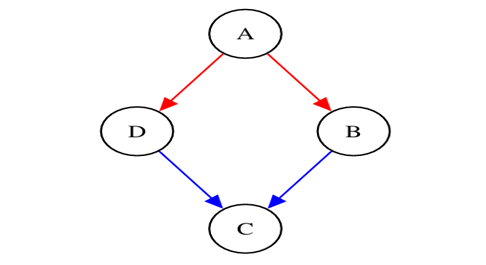
\includegraphics[width=1\linewidth]{DAG Sample 1.png}
    \caption{A diagram showing the relationships between nodes A, B, C, and D}
    \label{fig:DAG 1}
\end{figure}

In the above diagram, A, B, C, and D, are four random variables represented by nodes in the network of the graph. Node A is the parent of B, and C is B’s child. Node C is independent of A. These visuals are easy to understand for stakeholders, aiding in linking risk measurement and management within an institution.

Bayesian Networks satisfy the Local Markov Property (Pavan, 2024), where a node is conditionally independent of its non-descendants given its parents. 
For example, \[P(D\mid A, B) = P(D\mid A)\] since D is independent of B. This simplifies the Joint Distribution and leads to the concept of a Markov Random Field, a random field that follows Markov properties. 

\textcite{sohan2024conditional}, described the Conditional Probability of event A as the probability that event A will occur given that another event B has already happened. Conditional probability is the likelihood of an event occurring, given that another specific event has occurred.
 Based on probability theory, the conditional probability of an event A given event B is denoted as P(A/B). This measures the probability of event A when event B is known to have occurred, effectively reducing the sample space to only those outcomes where event B is true (Shankar, 2021). The formula defines the conditional probability. 
The conditional probability of event \( A \) given event \( B \) is defined as:
\begin{equation}
P(A \mid B) = \frac{P(A \cap B)}{P(B)}
\end{equation}
Here, \( P(A \cap B) \) represents the probability of both events A and B co-occurring (the intersection of A and B), and \( P(B) \) is the probability of event B occurring.

Bayes’ theorem, named after the Reverend Thomas Bayes, helps in determining the probability of an event based on the occurrence of another related event. In the context of this study, Bayes’ theorem is used to update our beliefs about the likelihood of a series of events or risks based on new information. Operational risks—those arising from failures in internal processes, systems, or external events—often rely on conditional probabilities that evolve as new data or incidents occur. Bayes’ formula exists for both events and random variables. Bayes’ theorem formulas are derived from the definition of conditional probability and can be applied to both discrete events \( A \) and \( B \), and continuous random variables \( X \) and \( Y \).

\begin{figure}[H]
    \centering
    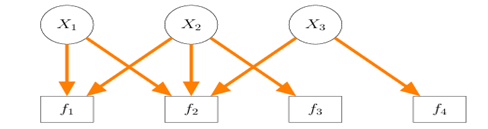
\includegraphics[width=1\linewidth]{DAC Sample 2.png}
    \caption{Conditional Probability and Bayesian Theorem}
    \label{fig: Bayesian Theorem}
\end{figure}

BNs describe the joint probability distribution over a set of variables, given the conditional dependencies/independencies contained in the graphical structure. Given a Bayesian Network (BN) with a set of variables: \( X = (X_1, X_1 \ldots X_n) \), where each variable \( X_i \) may depend on a subset of other variables, its “parents” in the network, denoted as \( \text{pa}(X_i) \), we can write the conditional probability distribution of each variable given its parents as \( P(X_i \mid \text{pa}(X_i)) \). The full joint probability distribution of the network is then the product of all these conditional probabilities. Mathematically, this is expressed as:

\begin{equation}
P(X_1, X_2, \ldots, X_n) = \prod_{j=1}^{n} P(X_i \mid x_{\text{Parents}(i)})
\end{equation}

\begin{equation}
= \prod_{j=1}^{n} P(X_i \mid \text{pa}(x_i))
\end{equation}

This formula is powerful because it allows us to compute the joint probability distribution of the entire set of variables by considering only the local conditional dependencies defined in the BN. This reduces the complexity of inference and calculation significantly, especially in large networks, by leveraging conditional independence relationships.


\section*{Explanation of Each Term}

\begin{enumerate}
    \item \( P(X_i \mid \text{pa}(X_i)) \): The probability of a variable \( X_i \) given its parents, i.e., the variables it directly depends on. If a variable \( X_i \) has no parents, then \( P(X_i \mid \text{pa}(X_i)) \) simplifies to \( P(X_i) \), since it has no dependencies.

    \item \( \prod_{j=1}^{n} \): The product notation signifies that we multiply the conditional probabilities for all variables in the network, from \( X_1 \) to \( X_n \).

    \item \( X = (X_1, X_2, X_3, \ldots, X_n) \): A collection of \( n \) random variables where each \( X_i \) belongs to a domain and is associated with factors \( f_1, f_2, \ldots, f_m \), and each \( f_i(x) \geq 0 \).

    \item The weight \( w(x) \) is defined as:
    \begin{equation}
    w(x) = \prod_{j=1}^{m} f_i(x)
    \end{equation}
    This represents the product of all factors evaluated at a particular configuration \( x \).
\end{enumerate}

\section*{Definition}

Therefore, by definition, let \( X = (X_1, \ldots, X_n) \) be a set of random variables. A Bayesian Network (BN) is a directed acyclic graph (DAG) that specifies a joint distribution over \( X_1 \) as a product of local conditional distributions, one for each node. 

\[
X = (X_1, X_2, X_3, \ldots, X_n)
\]

Considering \( n \) random variables \( X_1, X_2, X_3, \ldots, X_n \), a Bayesian Network would have \( n \) nodes where node \( j \) (with \( 1 \leq j \leq n \)) corresponds to the random variable. The joint probability of random variables in the BN would then be defined as:

\begin{equation}
\text{def} = \prod_{j=1}^{n} P(X_i \mid \text{Parents}(X_i))
\end{equation}

This defines a large joint distribution in a modular way, one variable at a time. The graph captures what other variables a given variable depends on. Then we specify a local conditional distribution for variable \( X_i \), which gives an assumption \( x_{\text{Parents}(i)} \) to its parents. Then the joint distributions are simply defined to be the product of all the local conditional distributions together. 

Bayes’ theorem allows the determination of posterior probabilities based on prior probabilities and the likelihood of an event given the causes.

\textbf{Prior probability}: Represents the strength of belief in a hypothesis or parameter value before data is gathered. It may also represent prior knowledge or information about an event \parencite{mikkola2024prior}.

\textbf{Posterior probability}: Represents how the investigator’s beliefs have changed after the data is considered. It is the probability of an event occurring given that another event has occurred \parencite{hart2022posterior}.

\subsection{Prior Distribution (Unconditional Probability Distribution) }
When using the Bayesian network for calculations, one should master well the Prior Bayesian formula and apply it with flexibility. The given formula below can be used to simplify the calculation of probability distribution in Bayesian Networks. The prior distribution of a variable \(X_i\) in a Bayesian Network is computed by marginalizing all other variables in the network. It is given by the following formula

\begin{equation}
p(X_i)=\sum_{F_x} \left[ p(X_i \mid pa(X_i)) \cdot p(F_x) \right]
\end{equation}
\begin{itemize}
    \item \( p(X_i) \) is the prior distribution of \( X_i \).
    \item \( F_x \) is the set of all other variables in the network.
    \item \( \text{pa}(X_i) \) denotes the parent nodes of \( X_i \).
    \item \( p(X_i \mid \text{pa}(X_i)) \) is the conditional probability of \( X_i \) given its parents.
    \item \( p(F_x) \) is the joint probability distribution of the other variables in the network.
\end{itemize}

\section*{Posterior Distribution (Conditional Probability Distribution)}

The posterior distribution represents the updated probability of a variable given some evidence \( E \). It is computed using Bayes' Theorem:

\begin{equation}
p(X_i \mid E) = \frac{p(E \mid X_i) \cdot p(X_i)}{p(E)}
\end{equation}

Where:
\begin{itemize}
    \item \( p(X_i \mid E) \) is the posterior distribution of \( X_i \) given the evidence \( E \).
    \item \( p(E \mid X_i) \) is the likelihood of the evidence \( E \) given \( X_i \), which is computed by summing over the conditional probabilities of the evidence given the parents of \( X_i \).
    \item \( p(X_i) \) is the prior distribution of \( X_i \) (as computed earlier).
    \item \( p(E) \) is the marginal likelihood of the evidence, computed by summing over all possible configurations of \( X_i \) and the other variables in the network:
    \begin{equation} 
    p(E) = \sum_{X_i} p(E \mid X_i) \cdot p(X_i)
    \end{equation}
\end{itemize}

\section*{Loss Distribution Approach (LDA)}

The Loss Distribution Approach is a statistical technique that estimates the distribution of losses based on historical data. The LDA assumes that operational losses are driven by two independent factors, the frequency and the severity of the event. The frequency is the number of loss events that occur in a given period, such as a year. The LDA works like this, we list all the things that could go wrong for a company, such as Fraud, system glitches, execution errors, and legal issues. Then we figure out how likely each event is and how much money it will cost. Then create a sort of overall Bayesian map showing the possible losses and decide how much money it needs to have on hand (kind of like a safety net) to cover unexpected financial loss from the potential issues. This could be a way to address what-ifs in the business world. The LDA captures tail risk, provides a quantitative measure of the operational risk exposure, and can accommodate different operational risk losses \parencite{hadley_selection_2019}. The mathematical expression below simplifies the loss distribution approach that banks use to set the Net capital requirement to offset the loss in the event of an unexpected business interruption. Using notation adapted from \textcite{embrechts2011modelling}, loss events are denoted as; 
\begin{equation}
\{X_{t,n}^{b,l}\}, \quad \text{for } t = 1, 2, \dots, 8; \quad l = 1, 2, \dots, 7; \quad n = 1, 2, \dots, N_t^{b,l}
\end{equation}
Where \( X_{t,n}^{b,l} \) is a random variable for the loss severity of the \(n^{\text{th}}\) loss event occurring in fiscal year \(t\) for the business line \(b\) and the event type \(l\), and \( N_t^{b,l} \) is a random random variable for the number of losses occurring in fiscal year \(t\) for business line \(b\) and event type \(l\). Thus, \( S_{T+1} \) is a random variable for firm-wide annual operational loss for next fiscal year and can be calculated as
\begin{equation}
S_{T+1} = \sum_{b=1}^8 \sum_{l=1}^7 \sum_{n=1}^{N_{T+1}^{b,l}} X_{T+1,n}^{b,l} = \sum_{b=1}^8 \sum_{l=1}^7 L_{T+1}^{b,l} 
\end{equation}
Where \( L_{T+1}^{b,l} \) is the annual loss for business line \(b\) and event type \(l\) in year \( T + 1 \). The goal of the LDA is to estimate the distribution of \( S_{T+1} \) via simulation and calculate RC as the 99.9\% quantile of this estimated distribution. There are two sources of randomness in \( S_{T+1} \), the loss frequency and the loss severity. The loss frequency, \( N_{T+1}^{b,l} \), is a discrete random variable for the number of losses occurring next fiscal year in business line \(b\) and event type \(l\). And the loss severity, \( X_{T+1,n}^{b,l} \), is a non-negative, continuous random variable as defined in (1). When calculating RC, we follow two common assumptions:

\begin{enumerate}
    \item \( N_t^{b,l} \) are independent of \( X_{t,n}^{b,l} \) for a given business line \(b\), event type \(l\), and year \(t\);
    \item \( \{X_{t,n}^{b,l}\} \) for \( t = 1,2,\dots,8; l=1,2,\dots,7; n=1,2,\dots,N_t^{b,l} \) are independent and identically distributed for a given business line \(b\), and event type \(l\).
\end{enumerate}

To estimate loss severity distributions, losses mapped to a given event type may be combined across business lines to produce an operational risk category (ORC), which is the level at which the banks model generates a separate distribution to estimate potential losses \parencite{hadley_selection_2019}.
Risk Severity is the extent of the damage to the institution, its people, and its goals and objectives resulting from a risk event occurring. The severity of risk is the degree of damage that could result from a risk event. Operational risk severity is a rating that businesses assign to risk based on their potential impact and likelihood of occurring. The severity of risk can be categorized as low, medium, or high. This allows risk managers to determine how much attention and resources should be devoted to managing risk.

\section*{Operational Loss Distribution}

Operational Loss Distribution models the aggregate financial losses resulting from operational risk events within a specified period, typically annually. The modeling process involves two key components: the frequency distribution, which estimates the number of loss events, and the severity distribution, which assesses the magnitude of each loss \parencite{cohen_estimating_2024}. By selecting appropriate statistical distributions for frequency (e.g., Poisson or Negative Binomial) and severity (e.g., Lognormal, Weibull, Gamma, or Generalized Pareto), financial institutions can simulate the overall loss profile through Monte Carlo methods or analytical convolution techniques \parencite{hadley_selection_2019}. This approach enables the estimation of the aggregate loss distribution, from which risk metrics such as Value-at-Risk (VaR) or Expected Shortfall (ES) can be derived. 

These metrics are crucial for determining the regulatory capital required to absorb extreme but plausible losses, with institutions often targeting high quantiles (e.g., the 99.9th percentile) to comply with regulatory standards. The Loss Distribution Approach (LDA), commonly employed under the Basel II and III frameworks, provides a structured methodology for quantifying operational risk. However, its effectiveness depends on the quality of loss data, appropriate model selection, and the consideration of tail events, ensuring that risk is neither underestimated nor overestimated, thus supporting sound capital planning and operational resilience.

\section*{Bayesian Network parameters determination}

Bayesian Network parameters to be quantified include state probabilities for root nodes and quantifying conditional probabilities (Conditional Probability Tables (CPT) or Conditional Probability Functions (CPF)) which model the probabilistic relationship between connected nodes. A quantified Bayesian Network can perform forward or backward inference, including diagnostic analyses with various inference algorithms based on Bayes’ theorem \parencite{moradi_integration_2022}.

Inference algorithms are divided into exact (message-passing, conditioning, junction tree, symbolic probabilistic inference, etc.) and approximate inferences (stochastic sampling, search-based algorithm, and loopy belief propagation algorithm). Learning parameters in a Bayesian network involves determining the conditional probability table for each node, assuming the network structure is already established. Traditionally, experts would estimate these probabilities using prior knowledge, but this approach can deviate significantly from empirical data. Modern techniques emphasize data-driven learning of these parameters, which enhances accuracy for further analysis. A key characteristic of Bayesian networks is their ability to directly represent real-world relationships rather than only focusing on reasoning processes \parencite{Chaoyu2020}.

\section*{Learning the Bayesian Parameters}

Learning the Bayesian parameters given a fixed network structure is a mammoth task, in statistics, and it requires substantial knowledge about Bayesian Statistical inference. According to the study on Learning Bayesian Network Model Structure from Data by \textcite{Margaritis2003}, priori distribution is assumed over the parameters of the local pdfs before the data are used. The conjugacy of a prior distribution is beneficial because it ensures that the posterior distribution belongs to the same family as the prior, but with updated hyperparameters \parencite{Dearden2013}. 

For multinomial distributions, the conjugate prior comes from the Dirichlet Family. Denoting the probability of each bin, \( p_{ijk}, k=1,\dots,r \) in the local probability density function of the variable \( X_i \) for the parent configuration \( pa_{ij} \), the Dirichlet distribution over these parameters is expressed by;

\begin{equation}
p_{ijk}, k=1,\dots,r | G = \text{Dir}(\alpha_{ij1}, \alpha_{ij2}, \dots, \alpha_{ijr}) = \frac{\Gamma(\alpha_{ij}) \prod_{k=1}^{r_i} p_{ijk}^{\alpha_{ijk}}}{\prod_{k=1}^{r_i} \Gamma(\alpha_{ijk})}
\end{equation}
Where \( \alpha_{ijk} \) are its hyperparameters and \( \alpha_{ij} = \sum_{k=1}^{r} \alpha_{ijk} \)

Assuming local and global parameter independence, the distribution over the set of parameters \( p \) of the entire BN is 
\begin{equation}
\Pr(p | G) = \prod_{i=1}^n \prod_{j=1}^{q_i} \frac{\Gamma(\alpha_{ij})}{\prod_{k=1}^{r_i} \Gamma(\alpha_{ijk})} \prod_{k=1}^{r_i} p_{ijk}^{\alpha_{ijk} - 1} 
\end{equation}

Conditional on the dataset \( D \), the posterior probability over the parameters is also a member of the Dirichlet family, since it is conjugate before the multinomial. It is

\begin{equation}
p_{ijk} | G,D = \text{Dir}(N_{ij1} + \alpha_{ij1}, N_{ij2} + \alpha_{ij2}, \dots, N_{ijr} + \alpha_{ijr})
\end{equation}

And 

\begin{equation}
\Pr(p | G) = \prod_{i=1}^n \prod_{j=1}^{q_i} \frac{\Gamma(\alpha_{ij} + N_{ij})}{\prod_{k=1}^{r_i} \Gamma(N_{ijk} + \alpha_{ijk})} \prod_{k=1}^{r_i} p_{ijk}^{N_{ijk} + \alpha_{ijk} - 1}
\end{equation}

Where \( N_{ij} \) represents the number of samples that fall into the \(k\)-th bin of the probability density function (pdf) for the variable \( X_i \), given that its parent nodes are in the \(j\)-th configuration (this is known as the sufficient statistic for that pdf). When using this distribution to predict the value of any quantity \( Q(X_1,X_2,\dots,X_n) \) that depends on the variables in the domain, you compute the prediction by averaging over all possible values of the (unknown) parameters—essentially integrating out the uncertainty in the parameters to make the prediction more robust.

\begin{equation}
\Pr(Q(X_1,X_2,\dots,X_n) | G,D) = \int Q(X_1,X_2,\dots,X_n) \Pr(P | G,D) dp
\end{equation}

More often, for reasons of convenience, the maximum likelihood (ML) parameters are used instead of the entire distribution. The ML for \( p_{ijk} \) is 
\begin{equation}
p_{ijk} = \frac{\alpha_{ijk} + N_{ijk}}{\alpha_{ij} + N_{ij}}
\end{equation}

Also, for convenience, especially in cases where data are abundant, the hyperparameters are ignored \( \alpha_{ijk} \ll N_{ijk} \) and the fraction \( \frac{N_{ijk}}{N_{ij}} \) is used instead. 

\section*{Learning the Structure: Score-based Methods}

One of the most popular methods of inducing BNs from data, especially for pdf estimation, is the score-based approach. The process assigns a score to each candidate BN, typically one that measures how well that BN describes the data set \( D \). Assuming a structure \( G \), its score is

\[
\text{Score}(G,D) = \Pr(G | D)
\]

in other words, the posterior probability of \( G \) given the data set. A score-based algorithm attempts to maximize this score. Computation of the above can be cast into a more convenient form by using Bayes’ law:

\begin{equation}
\text{Score}(G,D) = \Pr(G | D) = \frac{\Pr(D | G) \Pr(G)}{\Pr(D)}  
\end{equation}

To maximize this, we need only maximize the numerator, since the denominator does not depend on \( G \). There are several ways to assess \( \Pr(G) \) from prior information. 

To calculate \( \Pr(D | G) \), the Bayesian approach averages over all possible parameters, weighing each by its posterior probability as discussed above. As we mentioned above, score-based algorithms attempt to optimize this score, returning the structure \( G \) that maximizes it.

\section{Markov Chain Monte Carlo (MCMC)}
Markov Chain Monte Carlo (MCMC) is a group of algorithms that use Markov Chains to draw samples from probability distributions that provide elegant solutions to the Bayesian problems of prediction and model choice \parencite{gilks2001markov}. MCMC is based on a random walk to produce a sequence of models from the model space. The Markov chain aspect is that a new model is generated conditional on the previous one, and the process is independent of how the previous model was arrived at.

According to \textcite{karandikar2006mcmc}, and \textcite{gallagher2009markov}, the basis of MCMC is that we choose a model from some a priori specified range of the model parameters, and then propose a new model, conditional on the current model. From the proposed model, we then decide whether to replace or not to replace the current model with the proposed one. MCMC is particularly useful when direct sampling from a distribution is difficult or impossible, such as in high-dimensional spaces or when the distribution is complex \textcite{koop1997bayesian}. MCMC algorithms construct a Markov chain whose equilibrium distribution approximates the target probability distribution, meaning that the chain eventually settles into a distribution resembling the desired one. 

The causal discovery and Bayesian inference framework was developed by \textcite{annadani2023bayesdag}, \textcite{mclachlan2024approach}, and  \textcite{gilks2001markov}, and the framework addresses computational challenges in joint inference over the combinatorial space of DAGs and nonlinear functions, and demonstrates effectiveness through empirical evaluation on synthetic and real-world datasets. In this research, we focus on the Bayesian Network, determining the causal relationship amongst the risk variables. The BNN needs to be tested under different scenarios, where the MCMC will be used to develop a new model based on the current probability distributions. The fundamental goal is to predict a set of unobserved losses, given the current loss data and the assumed posterior distribution model. 
\subsection*{Bayesian Posterior Density}
Let;
\begin{itemize}
  \item \( \mathcal{M} \): be the Bayesian statistical model,
  \item \( \psi \in \Psi \): the parameter vector,
  \item \( \pi(\psi) \): the prior density,
  \item \( f(y \mid \psi) \): the likelihood of observed data \( y \),
  \item \( \pi(\psi \mid y) \): the posterior density.
\end{itemize}

By Bayes' theorem, the posterior distribution is given by: 
\begin{equation}
\pi(\psi \mid y) = \frac{f(y \mid \psi) \, \pi(\psi)}{m(y)}
\end{equation}
where the marginal likelihood (normalizing constant) is: 
\begin{equation}
m(y) = \int f(y \mid \psi) \, \pi(\psi) \, d\psi
\end{equation}
This integral is typically intractable in closed form.

Then we compute the Posterior expectations:
\begin{equation}
\mathbb{E}_{\pi}[h(\psi)] = \int h(\psi) \, \pi(\psi \mid y) \, d\psi 
\end{equation}
\begin{itemize}
  \item Posterior mean: \( h(\psi) = \psi \)
  \item Posterior second moment: \( h(\psi) = \psi \psi^\top \)
  \item Posterior covariance:
  \begin{equation}
  \mathrm{Cov}(\psi \mid y) = \mathbb{E}[\psi \psi^\top] - \mathbb{E}[\psi]\mathbb{E}[\psi]^\top    
  \end{equation}
\end{itemize}

\subsection*{MCMC Estimation}

Using Markov Chain Monte Carlo (MCMC),:
\begin{equation}
\left\{ \psi^{(1)}, \psi^{(2)}, \dots, \psi^{(M)} \right\} \sim \pi(\psi \mid y)
\end{equation}
Then estimate:
\begin{equation}
\hat{\mu}_M = \frac{1}{M} \sum_{m=1}^M h(\psi^{(m)}) \approx \mathbb{E}_{\pi}[h(\psi)]
\end{equation}

\section{Allocating Capital for Operational Risk }
The Reserve Bank of Zimbabwe has prescribed various soundness standards for operational risk management for banking and insurance institutions. According to the Technical Guidance on the Implementation of the Revised Capital Adequacy Framework in Zimbabwe (2011), the operational risk management framework should, at a minimum, include identification, measurement, monitoring, reporting, control, and mitigation frameworks for operational risk. It has been recommended that banks must hold capital for operational risk equal to a fixed percentage (denoted alpha) of average annual gross income over the previous three years, where \( GI \) is the average annual gross income and \( \alpha \) is the parameter relating the industry-wide level of required capital to the industry-wide level of annual gross income. 

\[
K_{\text{BIA}} = GI \times \alpha
\]

That’s the Basic Indicator Approach for calculating operational risk capital.


Operational risk regulatory capital (ORRC) is defined as the regulatory capital that a banking or insurance institution is required to hold against its exposure to operational risk and is calculated using the Advanced Measurement Approach (AMA). AMA is an advanced model-based approach used to measure a banking institution’s regulatory capital for operational risk, which requires approval by the Reserve Bank. The allocation mechanism is appropriately risk-sensitive and continues to reflect the operational risk profile of the legal entity and its contribution to the banking group and is implemented consistently, empirically supported, and continues to be relevant and stable over time.

\newpage
\section{Chapter Summary}
This chapter explores various theoretical groundworks of the Bayesian Network (BN) modeling as a robust framework for understanding key risks and quantifying operational risk in the banking and insurance sectors. Bayesian Networks, as probabilistic graphical models, use directed acyclic graphs (DAG) to represent conditional dependencies between random variables, making them ideal for capturing causal relationships and uncertainties in operational risk scenarios. 

From the Literature review, we explained the foundational concepts, such as Bayes' Theorem, joint probability distributions, and parameter estimation techniques, highlighting their role in visualizing and reasoning about causal probabilities. Insights from various authors emphasize the utilization of the Bayesian Networks in combining internal data, external data, and expert opinions to model the frequency and severity of operational losses, addressing challenges associated with scarcity of databases or incomplete datasets. Regulatory frameworks like Basel II and Solvency II are also discussed, emphasizing the adoption of BNs for integrating advanced risk quantification methodologies such as the Loss Distribution Approach (LDA), scenario analysis, and the Advanced Measurement Approach for capital allocation.

This Literature also reviews empirical applications of Bayesian Networks in operational risk management. Research findings suggest that BNs improve risk prediction, adaptability, and scenario analysis by dynamically updating probabilities with new evidence. They offer advantages over traditional linear models by capturing nonlinear dependencies and addressing the heavy-tailed nature of operational loss distributions. However, challenges such as the lack of rigorous validation methods, integration of real-world data, and limitations in addressing dynamic risk environments remain a challenge to financial institutions. 

Lastly, this literature concludes by emphasizing the potential of BNs to close the gaps in operational risk modeling through innovations like machine learning and automation, while also calling for further deep research which could enhance Bayesian Network models for better real-time risk quantification and validation.

The next chapter presents the methodologies that should be the main guide for the center of this research and how the study will be carried out. 


\chapter{Methodology}
This chapter outlines the research methodology adopted to achieve the objectives of this study. It includes the research design, data collection methods, analysis techniques, and tools used to construct and validate the Bayesian Network (BN) framework for quantifying operational risk management. The chosen methodology is grounded in theoretical principles and practical considerations to ensure that the study is robust, reliable, and capable of addressing the main objectives and research questions outlined in Chapter 1. As discussed earlier, the primary aim of this study is to build a model that helps us identify the appropriate risk factors and obtain measures of the parameters associated with the Bayesian Model framework, which we can use to estimate the level of operational risk that will exist in future periods
\section{Research Design}
A mixed-methods approach was employed, integrating qualitative and quantitative techniques to construct, quantify, and validate the Bayesian Network framework. A mixed-methods approach is a research methodology in its own right, as supported by other scholars \parencite{dawadi_mixed-methods_2021}. As a methodology, it includes philosophical assumptions to provide directions for collecting and analyzing data from multiple sources in a single study. Mixing two methods offers a significant advantage over relying solely on a single method, providing deeper and more comprehensive insights into research phenomena. By combining qualitative and quantitative approaches, researchers can uncover dimensions of complex problems that cannot be covered effectively by a single method \textcite{Poth2020}, and a mixed-method design effectively integrates multiple data sources, which can assist in studying complex problems.

The application of mixed-methods research (MMR) allows the researchers to seek a wide view of their study by enabling them to view a phenomenon from different perspectives and research lenses. The quantitative approach method helps the researcher to collect the data from a large number of participants; thus, increasing the possibility to generalize the findings to a broader magnitude of losses related to operational risk across different lines of business. The qualitative approach provides a deeper understanding of the issue being investigated, Quantitative research is controlled, obstructive, objective, and product-oriented, which aims at quantifying the variation of certain situations, issues, events, or phenomena. For this study, the quantitative approach uses statistical methods to measure and analyze the frequency and severity of loss events. By quantifying risk factors, organizations can develop models that estimate potential operational losses and assess the probability of various risk events occurring. This approach helps in data-driven decision-making, risk mitigation strategies, and determining capital reserves for operational risk. 
\subsection{Descriptive Analysis: }
To understand the operational risk landscape and identify key risk factors. Building a Bayesian Network for operational risk involves several key steps.  The first part, descriptive analysis was conducted to understand the operational risk landscape and identify the key risk factors that influence outcomes. This involves collecting and analysing data on past risk events, uncovering patterns, trends, and significant outliers that provide a comprehensive overview of the risk environment. This stage lays the foundation for the construction of the Bayesian Network.
\subsection{Model Construction}
The model construction stage begins by designing the Bayesian Network using causal relationships derived from expert opinions (qualitative data) and historical data (quantitative data). The network was structured as a directed acyclic graph (DAG), where nodes represent operational risk factors such as system failures, process inefficiencies, or external disruptions, and edges indicate the causal dependencies between these factors
\subsection{Probabilistic Quantification:} 
We established the BN structure, and probabilistic quantification was performed to assign probabilities to the nodes and their dependencies. This procedure involves combining empirical data, such as the frequency and severity of past losses, with expert judgment to estimate probabilities for events that lack sufficient historical data. (Amin, 2016). This step ensures that the Bayesian Network reflects realistic likelihoods and enables the model to provide quantitative risk assessments under various scenarios. Each risk varies in intensity or severity and has a broad range of financial effects on a company from different situations.
\subsection{Model validation}
The validation process ensures that the framework is accurate and practically applicable. This was achieved through simulations, where the model was tested under different hypothetical scenarios, and sensitivity analysis, which examines how changes in input probabilities affect the outcomes. The network should be validated against known operational risk scenarios to confirm its predictive reliability. Through this iterative process, the Bayesian Network evolves into a robust tool that accurately quantifies operational risk and supports effective risk management decisions. 
\section{Data Collection Methods}
Data on operational failures in the company's history are minimal and might not be available, particularly for low-frequency, high-impact events. And in some cases, data for collapsed companies might be completely unavailable. With limited data on operational losses, the data required for constructing the Bayesian Network framework is sourced through the following methods:
\subsection{Secondary Data Sources:}
In Zimbabwe, some financial institutions do not publicly publish their operational losses because they want to maintain customer relationships. Due to the company’s privacy, obtaining valid data on operational risk will be difficult because of ethical considerations. 
\begin{itemize}
\item Historical loss data from financial institutions (internal loss event databases).
\item Historical data from the Reserve Bank of Zimbabwe (RBZ) that is publicly available. 
\item Industry reports and publications, including Basel II/III guidelines and relevant literature.
\item Publicly available operational risk incident datasets.
\end{itemize}
\subsection{{Primary Data Sources:}}
Expert Elicitation: Semi-structured interviews with risk management professionals to identify causal relationships, risk drivers, and their interdependencies.
Workshops: Focus groups with operational risk managers to validate the identified nodes and relationships in the BN framework.

\section{Model Development Approach}
The proposed quantification approach offers several advantages over methods relying only on historical data for assessing risk exposure. One key benefit is the ability to map risk flows and associated parameters, which allows for the seamless integration of changes in the company’s risk environment, such as adjustments to the model structure, the implementation of mitigation measures, and organizational transformations into the analysis. This adaptability ensures that the model remains relevant and reflective of the current situation. 

The risk assessment can be undertaken by combining different sources, such as expert opinions and internal and external historical data, to best describe the current risk environment. By synthesizing these varied inputs, the model captures nuances that purely historical approaches might overlook. This method facilitates the detailed analysis of complex production networks, offering insights into their true risk exposure. It not only identifies and evaluates drivers of operational risk but also quantifies the risk, providing a clear understanding of the organization’s risk profile.

Constructing the structure (topology) of a Bayesian network is shown in the \ref{fig:Structure (topology) of a Bayesian network}.
\newpage
\begin{figure}[H]
    \centering
    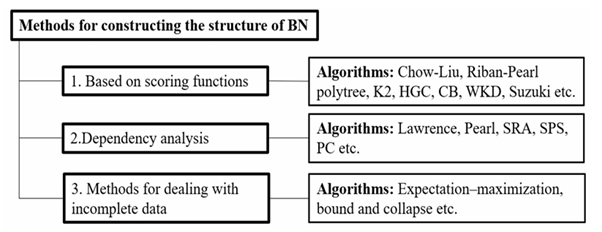
\includegraphics[width=1\linewidth]{Structure (topology) of a Bayesian network.png}
    \caption{Structure (topology) of a Bayesian network}
    \label{fig:Structure (topology) of a Bayesian network}
\end{figure}
The process of constructing the structure of a Bayesian Network (BN) can be approached using three main methods. The first method relies on scoring functions, where different candidate network structures are evaluated based on a score that balances how well the structure fits the data and its complexity, with algorithms like K2, Chow-Liu, and Hill Climbing being commonly used (Levenchuk, 2022). 

The second method is dependency analysis, which directly identifies statistical dependencies and independencies between variables using data-driven tests and then constructs the network to reflect these relationships, with algorithms such as the PC algorithm, Pearl’s method, and SRA playing key roles. 

The third method deals with incomplete data, where techniques like the Expectation-Maximization (EM) algorithm estimate both the missing data and the network structure iteratively, ensuring that incomplete observations do not compromise the learning process. These methods, whether applied individually or in combination, form the foundation for learning the causal structure that underpins a Bayesian Network.
\subsection{Structural Design:}
Finding the structure that best fits the data becomes one of the problems to solve when using BNs. Two types of machine learning perform this task: structural learning, which acquires the network structure (trees, polytrees, or multiconnected networks) from the data; and parametric learning, which has the associated conditional probabilities (table of probability) of each root node and the other variables. To determine the probability distributions linked to each vertex of the network, it is necessary to know the type of network; that is, these two learning approaches cannot be carried out independently (Muñoz-Valencia et al., 2023).
\subsection{Node Identification;} 
Creating the risk profile of each node in the Bayesian network is the first step in this process. Risk profiles are created by combining all sources of operational risk that can affect the same node and provide a basis for comparative assessment of these nodes. Mapping operational risk factors (nodes) such as internal fraud, system failures, and external events based on literature and expert input requires substantial expert knowledge. At each node, two separate tasks are performed: computation of the risk inherent to that node due only to its risks, and compounding it with the risk exposure of all incoming flows into that node. The compounded risk exposure also contributes to the mitigation efforts at that node to lower the risk exposure. This compounded risk exposure is then associated with the outgoing flow from that node. 
\subsection{Dependency Mapping:}
Establishing parent-child relationships between nodes using causal analysis. Dependency mapping and graph construction are critical steps in building a Bayesian Network. This involves identifying and establishing parent-child relationships between nodes based on causal analysis, as highlighted in Chapter 2. This step focuses on understanding how different key risk factors influence each other, determining which factors act as "parent" nodes (causal drivers) and which are "child" nodes (effects or outcomes). These relationships can be derived through expert judgment, historical data, or a combination of both, ensuring that the network accurately reflects the real-world risk profiles in financial institutions. 
\subsection{Graph Construction:} 
Creating a directed acyclic graph (DAG) that represents the identified dependencies.  The DAG visually represents the structure of the Bayesian Network, with nodes corresponding to risk factors and directed edges indicating causal dependencies between them. The acyclic nature of the graph ensures that there are no feedback loops, preserving the logical flow of cause-and-effect relationships. This graphical representation serves as the foundation for probabilistic quantification and further analysis.
\subsection{Network structure learning}
The network structure of a Bayesian Network (BN) associated with a data set can be learned using algorithms such as the grow-shrink algorithm or the hill climbing algorithm, both of which are known to produce different network structures as demonstrated by Leo, Sharma \& Maddulety (2020). The grow-shrink algorithm identifies each variable's Markov Blanket through an iterative process of adding and removing nodes based on conditional independence tests. The hill-climbing algorithm starts with an initial structure and iteratively modifies it (adding, removing, or reversing edges) to maximize a scoring function. 

Although automated structure learning is common and efficient in many fields, certain domains require the incorporation of expert knowledge, where the structure is manually defined to better reflect domain-specific causal relationships. This manual approach ensures the network aligns with expert understanding, especially in contexts like risk management or healthcare. Once the structure is learned or defined, visual examination of the resulting graph can provide valuable insights into the network’s properties and dependencies. 
\section{Quantification of Probabilities}
\subsection{Conditional Probability Tables (CPTs): }
For each node, CPTs are constructed to represent the likelihood of various outcomes based on parent node states (Sanford and Moosa, 2012). It is essential to assign probability distributions to the nodes and specify their parameters. These values should accurately represent both marginal and conditional probabilities relevant to the specific context. Such distributions can be established through experimental findings within the field, analysis of observed events, historical data, or insights provided by subject matter experts. 

\subsection{Probability Elicitation: }
Combining expert judgment with statistical techniques to estimate probabilities where data is scarce. Such probabilistic judgments are often used to provide information that cannot be obtained directly from data, observation, or first principles \parencite{Hora2017}. Probability elicitation is the most challenging part of constructing BN models, especially when there is limited availability of data like cybersecurity and when it relies on expert knowledge.  Therefore, we need to elicit probability for every possible combination of parent variables to complete the CPT of a child variable from experts, \parencite{chockalingam_probability_2023}. Using loss data and expert opinions, the Bayesian methodology can estimate operational risk loss distributions. The elicitation process of expert opinion allows a better understanding and sharing of operational risk.
\section{Data Analysis}
Cleaning and preparing an Operational risk dataset is often a mammoth task due to inconsistencies across industries, and companies. The nature of the data for modeling operational risk is the incurred losses by risk type gathered from historical data and expert elicitation as discussed earlier. Since the external and internal data may come in different formats, data transformation is necessary before the analysis. Data transformation and filtering is a mandatory step and the filtered data can then be grouped based on the classes of key risks defined. Inference in the Bayesian Network is performed to analyze the impact of different risk scenarios. Once the network has been built, we predict the probability of outcomes given initial conditions, the results should be diagnosed to estimate the most likely causes for observed outcomes.
\section{Model Validation}
Various methods were used to check and confirm the model's accuracy. Verification of the BN ensures the model functions as expected and involves manually reviewing simulation results for specific parts of the model. Adjusting parameters, like the frequency or severity of disruptions, and observing the expected outcomes also helped verify the model. Risk management professionals review the model structure and outputs to ensure alignment with real-world operational risk dynamics. After fitting the model, performance metrics were evaluated to assess how well the model's predictions align with real-world data. This involves comparing the predicted risk levels to actual loss outcomes and checking whether the predicted probabilities match the observed frequency of events. These steps help ensure the model is accurate and reliable for practical use.
\section{Scenario Analysis }
According to \textcite{Amin2016}, who asserts that each operational risk can vary in intensity or severity and has a broad range of financial effects on a company from different scenarios. Each risk event is more likely to happen under different situations, which we should consider when assessing the strength of the BN framework. Firstly, we developed discrete risk scenarios for each key risk. Each risk scenario describes a risk event, the likelihood of its occurrence, and the financial impact it has on the company. Sensitivity analysis was conducted by varying probabilities and observing changes in risk predictions. Simulations were run to evaluate the effect of hypothetical scenarios, such as cyberattacks or system failures, on operational risk.
\section{Ethical Considerations}
The study adheres to strict ethical standards in data collection and analysis, prioritizing confidentiality by maintaining the anonymity of participating experts and institutions. It ensures data integrity by relying on credible sources and verifying data accuracy. Additionally, informed consent is obtained from all participants involved in data elicitation from experts, ensuring their voluntary and informed participation.
\section{Limitations of the Methodology}
There are several challenges associated with using historical data and simulations for operational risk quantification. 
Historical data on operational failures within a company are often scarce or unavailable, especially for low-frequency, high-impact events. External loss data, while potentially useful, is difficult to apply directly due to variations in company size, risk culture, controls, and processes. Scaling external data to reflect the company’s current risk profile is complex and requires careful adjustments. 

Relying on historical data assumes that the past is a reliable predictor of the future. This can lead to the underrepresentation of unprecedented events and the overrepresentation of frequently occurring events that may have already been mitigated. The absence of data from collapsed companies introduces survival bias, and the limited data available makes it difficult to produce a good statistical BN model.

While valuable for quantitatively assessing risks, simulations also face limitations. They require detailed information about the statistical distributions and interdependencies of risks. In the absence of such information, the validity of the simulation results becomes questionable, as highlighted by the principle of "garbage in, garbage out." Moreover, risks can occur under a wide range of scenarios, and the intensity and severity of a given risk vary significantly across these scenarios. This variability adds further complexity to the modeling process.

Methods that rely on single correlation assumptions fail to capture the interdependencies between different risk scenarios and overlook the tendency of extreme events to co-occur across multiple risks. This lack of granularity in modeling correlations can lead to underestimating the compounding impact of concurrent extreme events, which are often critical in understanding operational risk. 
 
 \subsection{Tools and Software }
\begin{itemize}
    \item Python
    \item Excel
    \item Bayes Server Apk
    \item pgmpy, bnlearn
\end{itemize}
\section{Chapter Summary}
This chapter outlines the methodology used to construct, quantify, and validate a Bayesian Network (BN) framework for operational risk assessment. A mixed-methods approach integrates qualitative and quantitative techniques, leveraging historical data and expert elicitation to build a robust model.  

The model construction process begins with identifying key operational risk factors and mapping causal relationships using a Directed Acyclic Graph (DAG). Conditional Probability Distributions (CPDs) were defined through quantitative learning, combining statistical inference with expert judgment to estimate dependencies within the network. 

To quantify probabilities, empirical loss data and expert assessments were used to determine risk exposure, accounting for limited historical data. Scenario analysis and Monte Carlo simulations were run to assess the impact of various risk events, while sensitivity analysis ensures the model's robustness by examining how changes in probabilities affect outcomes. Model validation was conducted through back-testing, expert reviews, and performance metrics to ensure predictive reliability. Ethical considerations, including data confidentiality and informed consent, were upheld throughout the study.  

Despite its strengths, the methodology faces limitations, such as data scarcity, survival bias, and challenges in modeling interdependent risks. Nonetheless, the Bayesian approach provides a dynamic, data-driven framework for quantifying operational risk and supporting financial institutions in risk mitigation strategies.


\chapter{Data Analysis}
\section{Introduction} 
This chapter presents the analysis of operational risk loss data from 1980 to 2024, using the Bayesian Belief Network and focusing on major risk event types as described in Basel II and the ORX global report database. The objective is to explore the structure of the Bayesian model framework, quantification of the network, probability eliciting, validations of estimates, structural model building, risk process mapping and node identification, network structure, conditional probabilities and node discretion tables, and model structure validation.To gain insights applicable to managing operational risk in the banking sector, the study employs both descriptive and inferential statistical techniques in combination with causal structure learning. This section of the research is organized into two core components: data preprocessing (including exploration and transformation) and model development. Moreover, the chapter aligns with the research goals and objectives as outlined in Chapter 1. 

\subsection{Data Exploration}
\subsubsection{Risk Category and the dataset structure}
The structure of our dataset is as follows, we have 7 key risk categories which are identified as; Internal Fraud (IF), External Fraud (EF), Employment Practices and workplace safety (EPWS), Clients, Products and Business Practices (CPBP), Disasters and Public Safety (DPS) Technology and Infrastructure Failure (TIF) Execution, Delivery and Process Management (EDPM). Dataset structure: The data represents operational risk losses across seven risk categories tracked over seven years (1980-2024). The dataset contains numeric loss amounts presented in (thousands USD).

\begin{table}[h]
    \centering
    \begin{tabular}{lrrrrrrr}
        \hline
        \textbf{Date} & \textbf{Intfraud} & \textbf{Exfraud} & \textbf{EmployPWS} & \textbf{ClientsPBP} & \textbf{Disaster} & \textbf{ICTFailure} & \textbf{ExecutionDP} \\
        \hline
        1980 & 98.90 & 465.20 & 76.70 & 1816.40 & 40.00 & 50.30 & 407.50 \\
        1981 & 890.90 & 589.20 & 291.00 & 18275.00 & 9.40 & 3851.00 & 9353.10 \\
        1982 & 950.00 & 7045.20 & 3394.70 & 26504.30 & 389.70 & 844.40 & 13655.60 \\
        1983 & 161.10 & 304.40 & 233.80 & 2456.20 & 2.10 & 27.60 & 886.60 \\
        1984 & 158.40 & 4514.00 & 240.00 & 12962.00 & 30.30 & 678.40 & 5425.10 \\
        1985 & 11.20 & 104.10 & 26.90 & 75.50 & 3.80 & 507.20 & 729.10 \\
        1986 & 2.10 & 104.10 & 68.80 & 942.90 & 3.40 & 52.70 & 1970.90 \\
        \hline
    \end{tabular}
    \caption{Operational Risk Dataset Structure}
    \label{tab:Operational Risk Dataset Structure}
\end{table}
\section{Descriptive Statistics}
Table 4.2 shows the descriptive statistics of the variables available in our dataset. To establish a clear understanding of the nature of the dataset and the general statistics, box plots, frequency distributions were calculated for the 7 variables of the operational risks. These variables include the total operational risk loss (loss), Measures of central tendency (mean and median), dispersion (standard deviation and range), and distribution shape (minimum, maximum, and quartiles) were calculated.
\begin{table}[H]
\centering
\begin{tabular}{|l|r|r|r|p{5cm}|}
\hline
\rowcolor{gray!20}
\textbf{Variable} & \textbf{Mean} & \textbf{Min -- Max} & \textbf{Std Dev} & \textbf{Insight} \\
\hline
Internal Fraud  & 451.26 & 2.1 -- 997.3 & 304.55 & Moderate average; some extreme spikes. \\
External Fraud  & 3,511.78 & 4.4 -- 9,441.8 & 2,955.74 & Wide spread and very high outliers. \\
Employee Safety  & 2,203.58 & 26.9 -- 4,900.1 & 1,691.41 & Steady increase over time is likely; moderate spread. \\
ClientsPBP & 13,629.87 & 75.5 -- 26,863.3 & 8,294.86 & Highest average and widest range, indicating heavy losses. \\
Disaster & 247.88 & 0.4 -- 678.8 & 218.63 & Low average but high variability; large, rare events. \\
ICT Failures & 1,801.64 & 27.6 -- 3,926.4 & 1,309.33 & High variability; significant systemic impact possible. \\
Execution Errors  & 6,596.26 & 407.5 -- 14,879.2 & 4,428.29 & Very wide range; suggests frequent large-scale process failures. \\
\hline
\end{tabular}
\caption{Operational Risk Variables - Summary Statistics}
\label{tab:Operational Risk Variables - Summary Statistics}
\end{table}


The Table \ref{tab:Operational Risk Variables - Summary Statistics} shows mean, standard deviation, and range for each risk type, offering a view of the scale and volatility of operational losses. Each variable including Internal Fraud, External Fraud, Employee Practices and Workplace Safety, Clients/Products/Business Practices, Disaster, ICT Failure, and Execution \& Delivery Processes is represented with measures such as count, mean, standard deviation, minimum, and maximum values, and quartiles (25\%, 50\%, and 75\%). This data indicates substantial variability across risk categories, with ClientsPBP and ExecutionDP showing the highest means and standard deviations, highlighting their dominant contribution to overall risk. This description highlights the relative contributions of each risk event type to the overall operational risk

\begin{figure}[H]
    \centering
    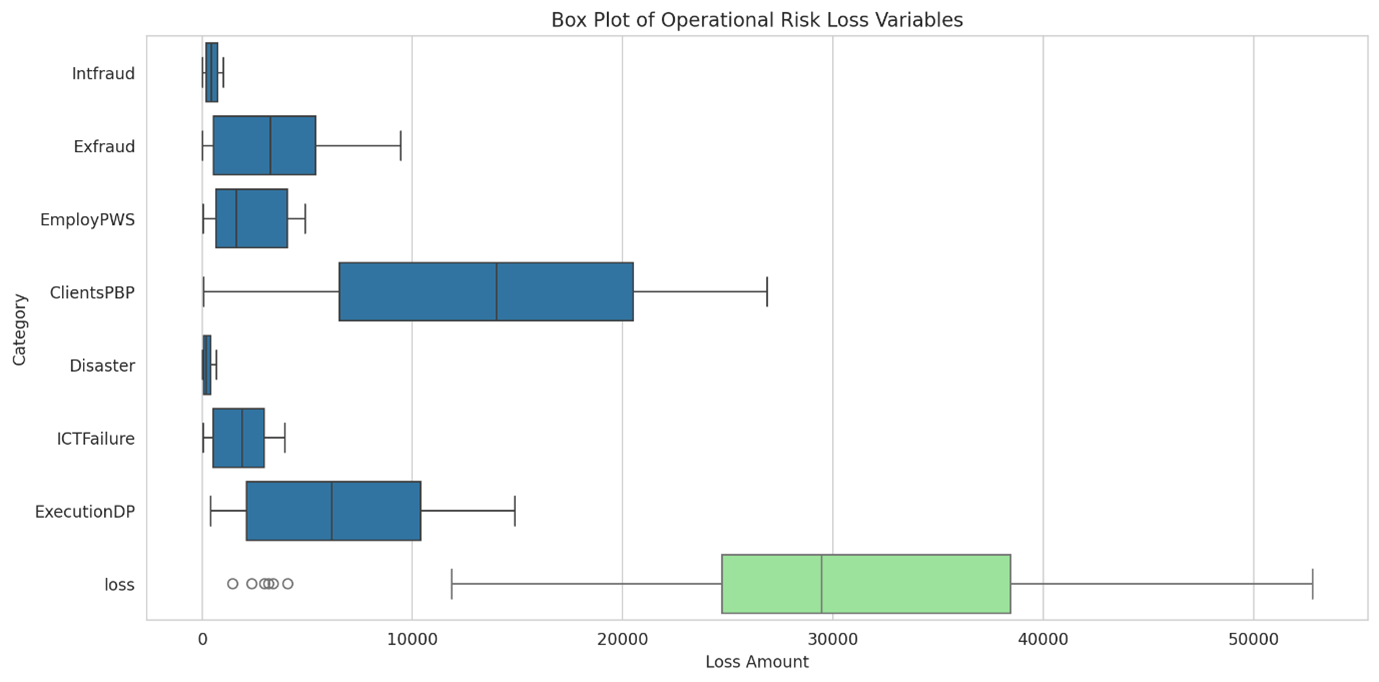
\includegraphics[width=1\linewidth]{Box Plot ORX Loss Variables.png}
    \caption{Box Plot of ORX Loss Variables}
    \label{fig:Box Plot of ORX Loss Variables}
\end{figure}

This box plot displays the distribution of operational risk losses across seven categories as outlined in Table 4.1. From the plot, each horizontal box shows the median (center line), interquartile range (colored box representing middle 50\% of data), and whiskers extending to minimum and maximum values within 1.5 times the interquartile range, with outliers as individual points. This visualization helps to quickly identify which operational risk categories have the highest median losses, greatest variability, and most extreme outliers, with Client/Business practice issues appearing to have both high median values and significant variability compared to categories like Disaster, which shows lower overall values.

\subsection{Frequency distributions}
The Figure below describes the frequency distributions of the operational risk variables. The bar graphs highlight how often certain ranges of these risk indicators occur. The line plots show the overall trend across those ranges. 

\begin{figure}[H]
    \centering
    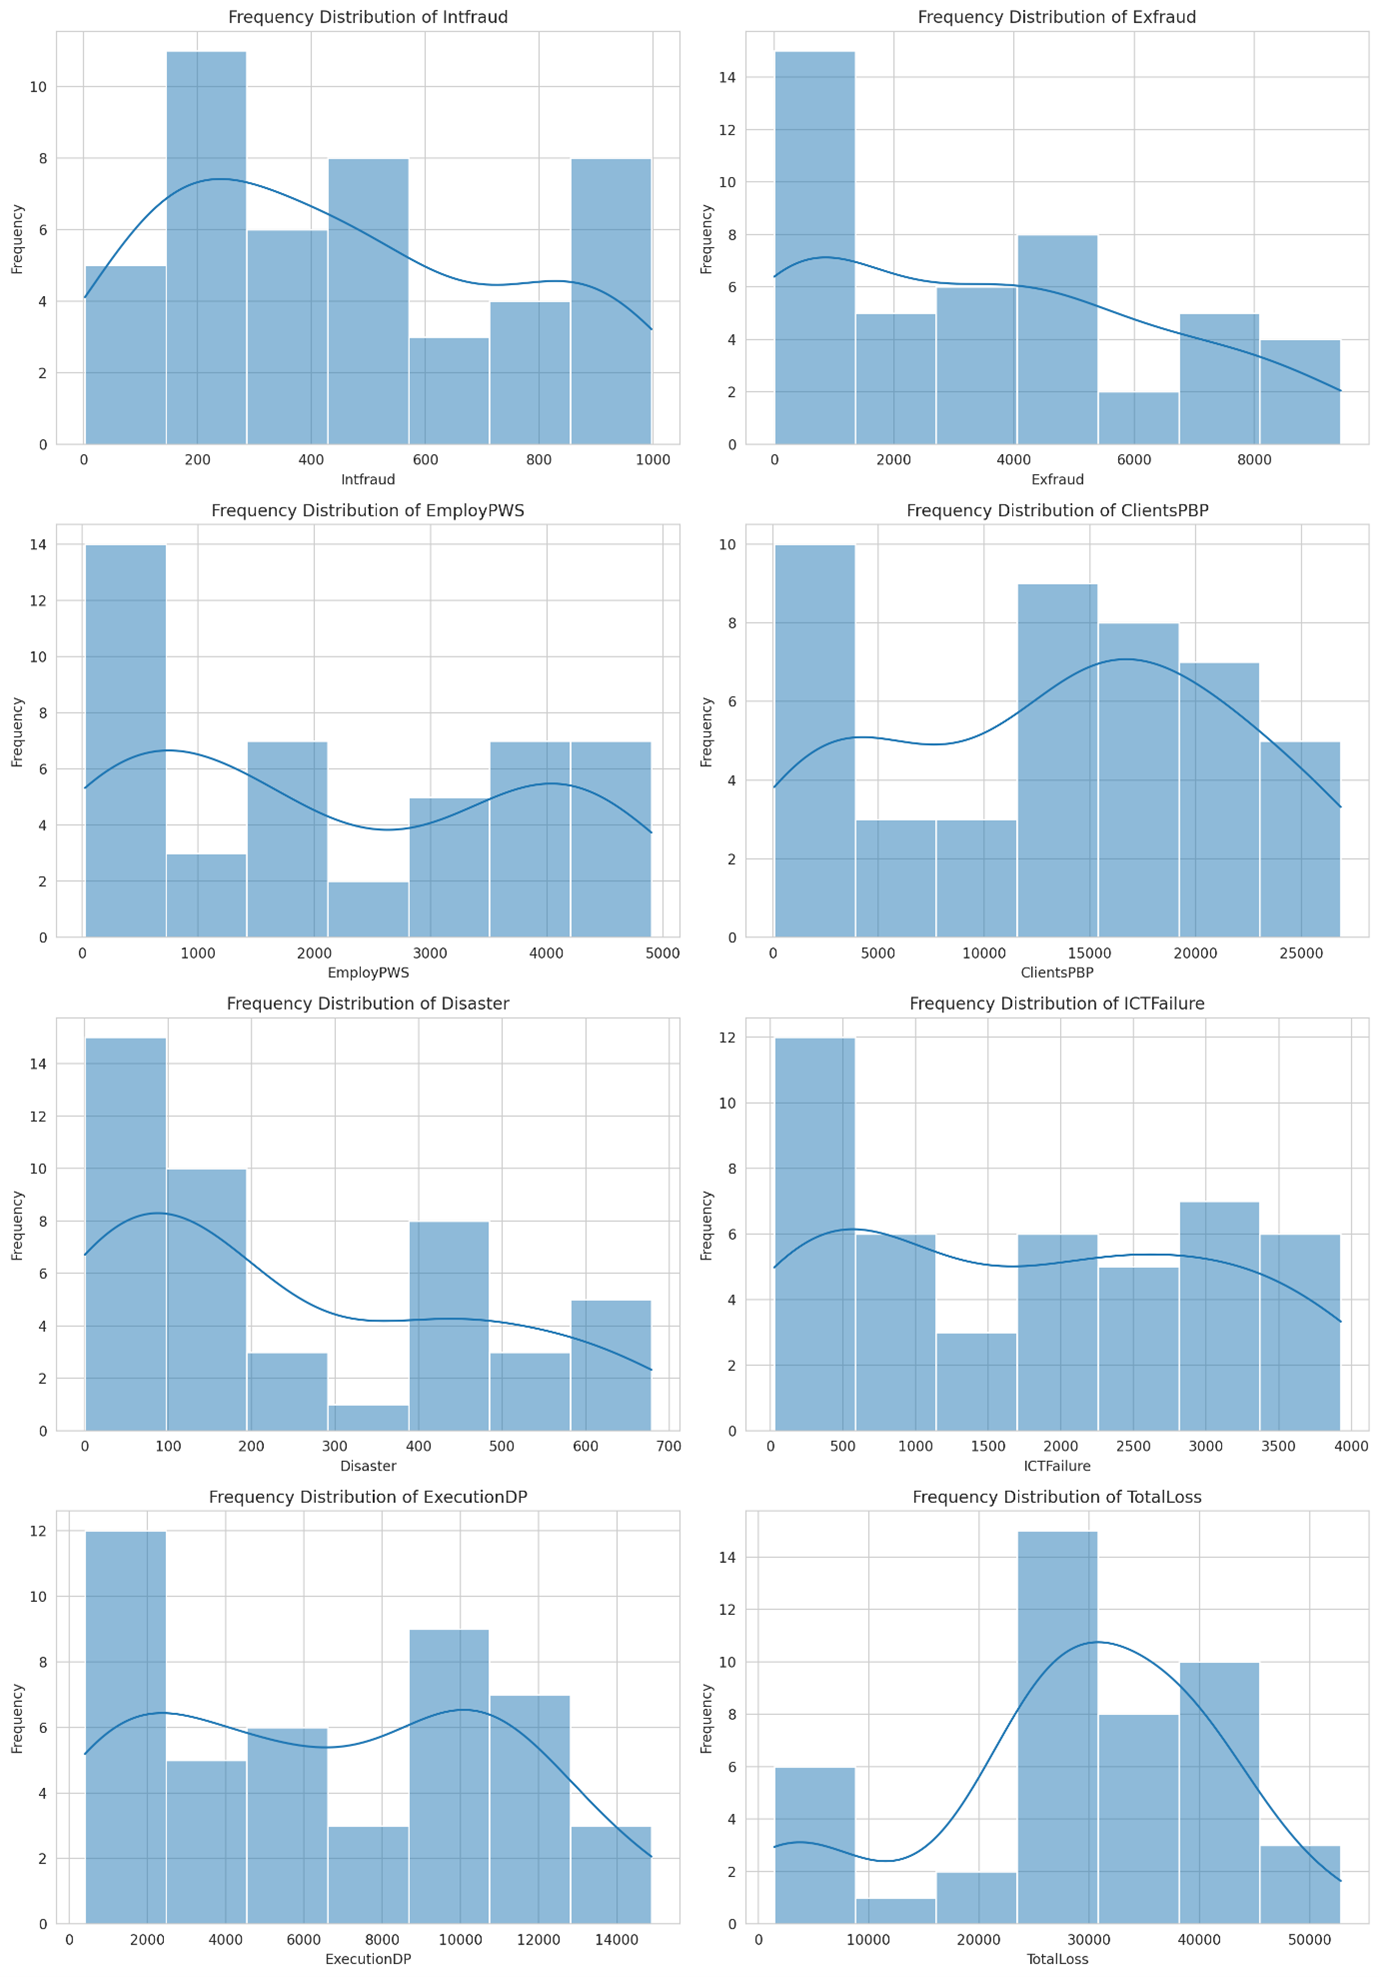
\includegraphics[width=0.75\linewidth]{Frequency Distributions ORX.png}
    \caption{Frequency Distributions ORX}
    \label{fig:Frequency Distributions ORX}
\end{figure}
\subsection{Correlation Matrix Analysis}
Pearson correlation coefficients were calculated between loss types

\begin{figure}[H]
    \centering
    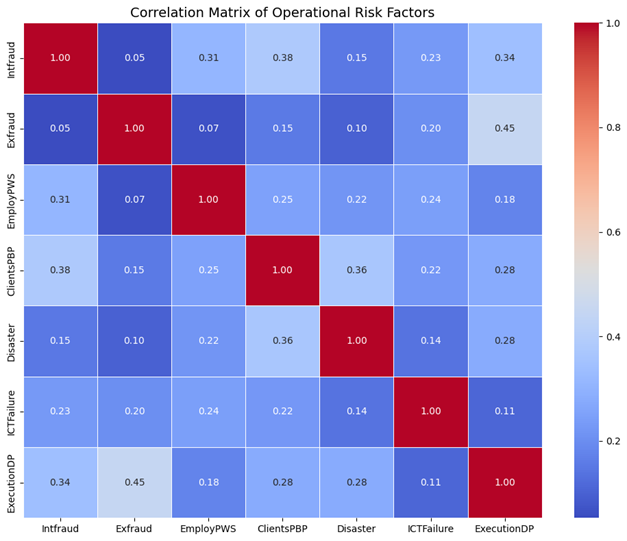
\includegraphics[width=0.75\linewidth]{Correlation Matrix.png}
    \caption{Correlation Matrix}
    \label{fig:Pearson correlation Matrix}
\end{figure}

The Pearson Correlation Matrix features are highly self-correlated (correlation of 1 along the diagonal). Most features have low correlations with each other, indicating they are relatively independent, and the strongest off-diagonal correlation is between "ExecutionDP" and "Exfraud" (0.45). Other notable correlations include "ClientSPB" with "Disaster" (0.36) and "ClientSPB" with "ExecutioDP" (0.28).
\section{Model Structural Design:}
\subsection{Bayesian Inference Model}
The priors for each operational risk indicator have been defined with distinct distributions. Each risk variable has been assigned a unique prior distribution rather than using the same prior across all variables. Different operational risk factors behave differently in the real world. Fraud events might be rare but severe, while process execution errors may be frequent but low in severity. We have used these distinct priors to incorporate these expectations into the model. The inference was carried out using the Bayesian maximum likelihood estimator to run and plot the prior distributions. 
\begin{figure}[H]
    \centering
    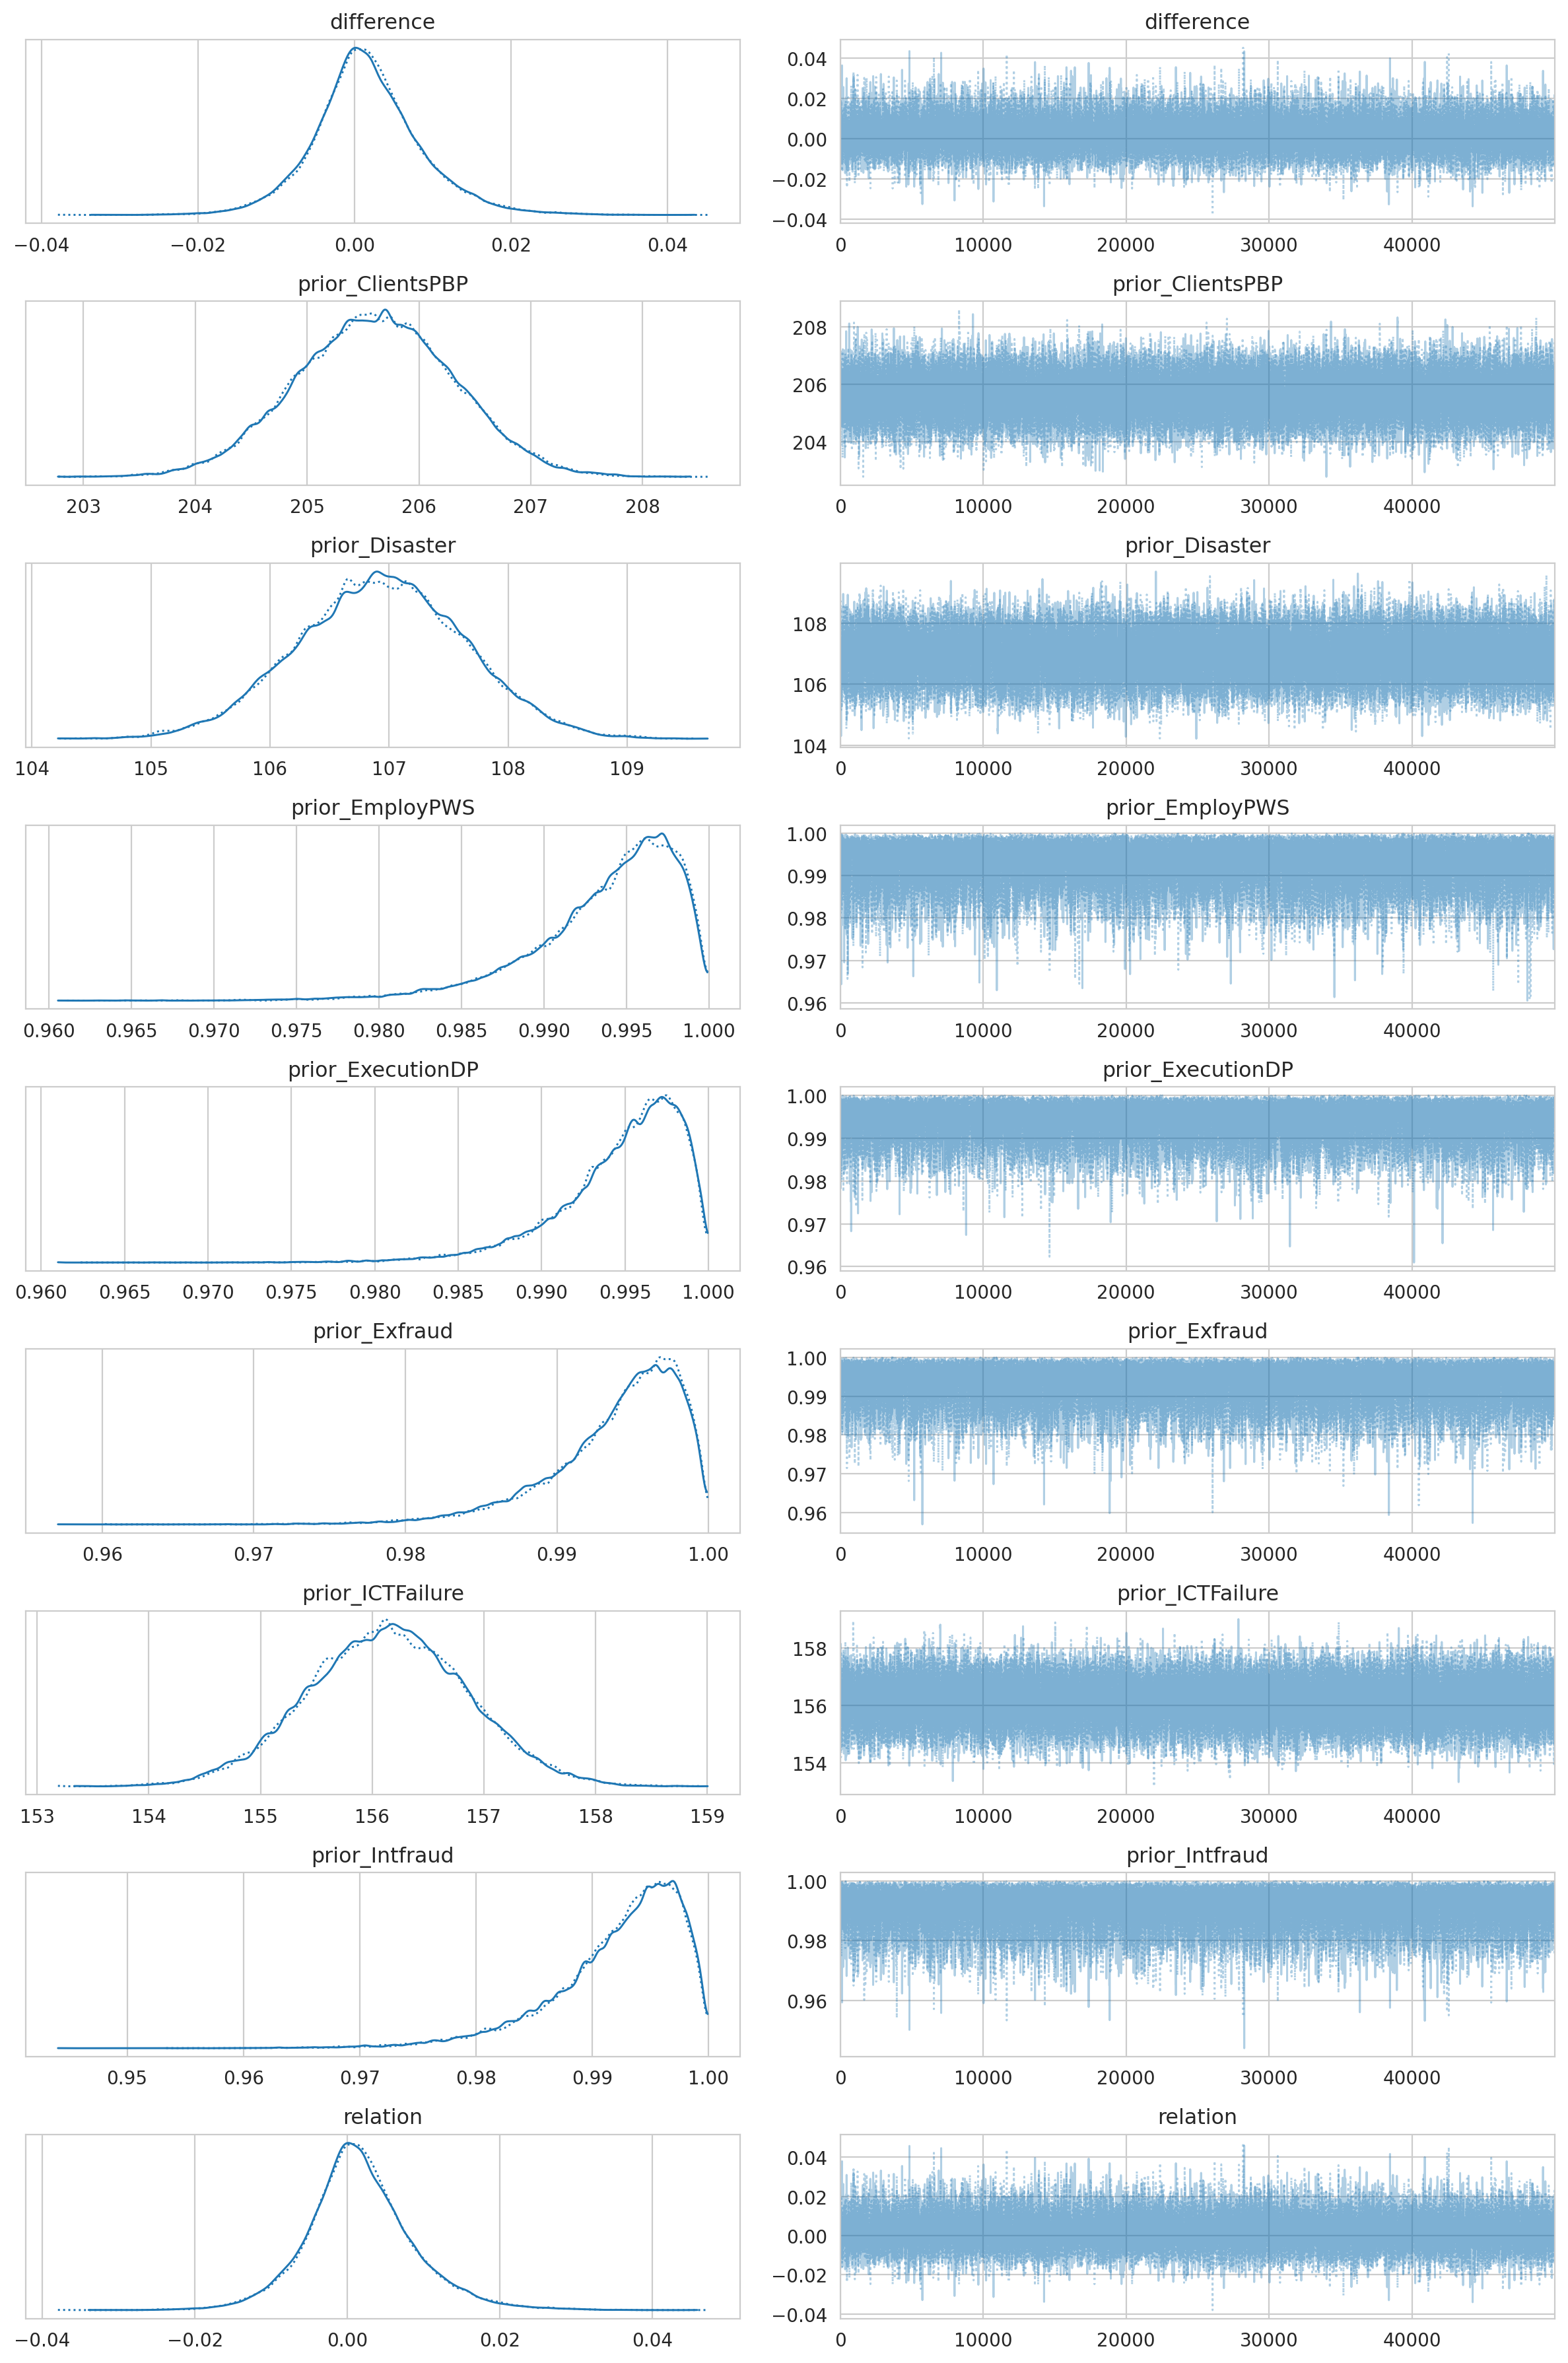
\includegraphics[width=1\linewidth]{Inference Model Prior vs Differences.png}
    \caption{Prior distributions vs Differences}
    \label{fig:Inference Model Prior vs Differences}
\end{figure}

The visualization in \ref{fig:Inference Model Prior vs Differences} displays MCMC diagnostic plots for a Bayesian model analysing risk factors. The left column shows prior density distributions for various parameters (ClientsPBP, Disaster, EmployPWS, ExecutionDP, Exfraud, ICTFailure, Intfraud), plus "difference" and "relation" parameters. The right column shows the corresponding trace plots of MCMC samples across iterations. The parameters show distinct distribution shapes - ClientsPBP, Disaster, and ICTFailure exhibit roughly symmetric bell curves centred around 205-206, 106-107, and 156, respectively, while EmployPWS, ExecutionDP, Exfraud, and Intfraud display right-skewed distributions with values concentrated near 1.0.

The trace plots suggest good MCMC convergence for most parameters, consistent mixing, and stable sampling across the 45,000+ iterations. The chains appear to be exploring the parameter spaces effectively without obvious trends, there are some visible autocorrelation in the sampling patterns. The difference and relation parameters are close to zero with symmetric distributions, indicating potentially null effects or standardized comparison metrics. The consistent sampling behaviour across different parameters suggests the model has reached a stable posterior estimation, though the exact interpretation would depend on the specific modeling context and parameterization used.
\subsection{Posterior distributions}
The visualization in Figure \ref{fig: Posterior Bayes Distributions} represents the posterior distributions of seven risk factors with their respective 94\% highest density intervals (HDI). Each distribution shows right-skewed patterns with mean values ranging from 0.91 (EmployPWS) to 0.98 (Exfraud), indicating high probability estimations across all factors. The HDI ranges vary in width, with EmployPWS showing the widest interval (0.84-0.98), suggesting greater uncertainty, while Exfraud displays the narrowest interval (0.94-1.0), indicating more precision in its estimation.
\begin{figure}[H]
    \centering
    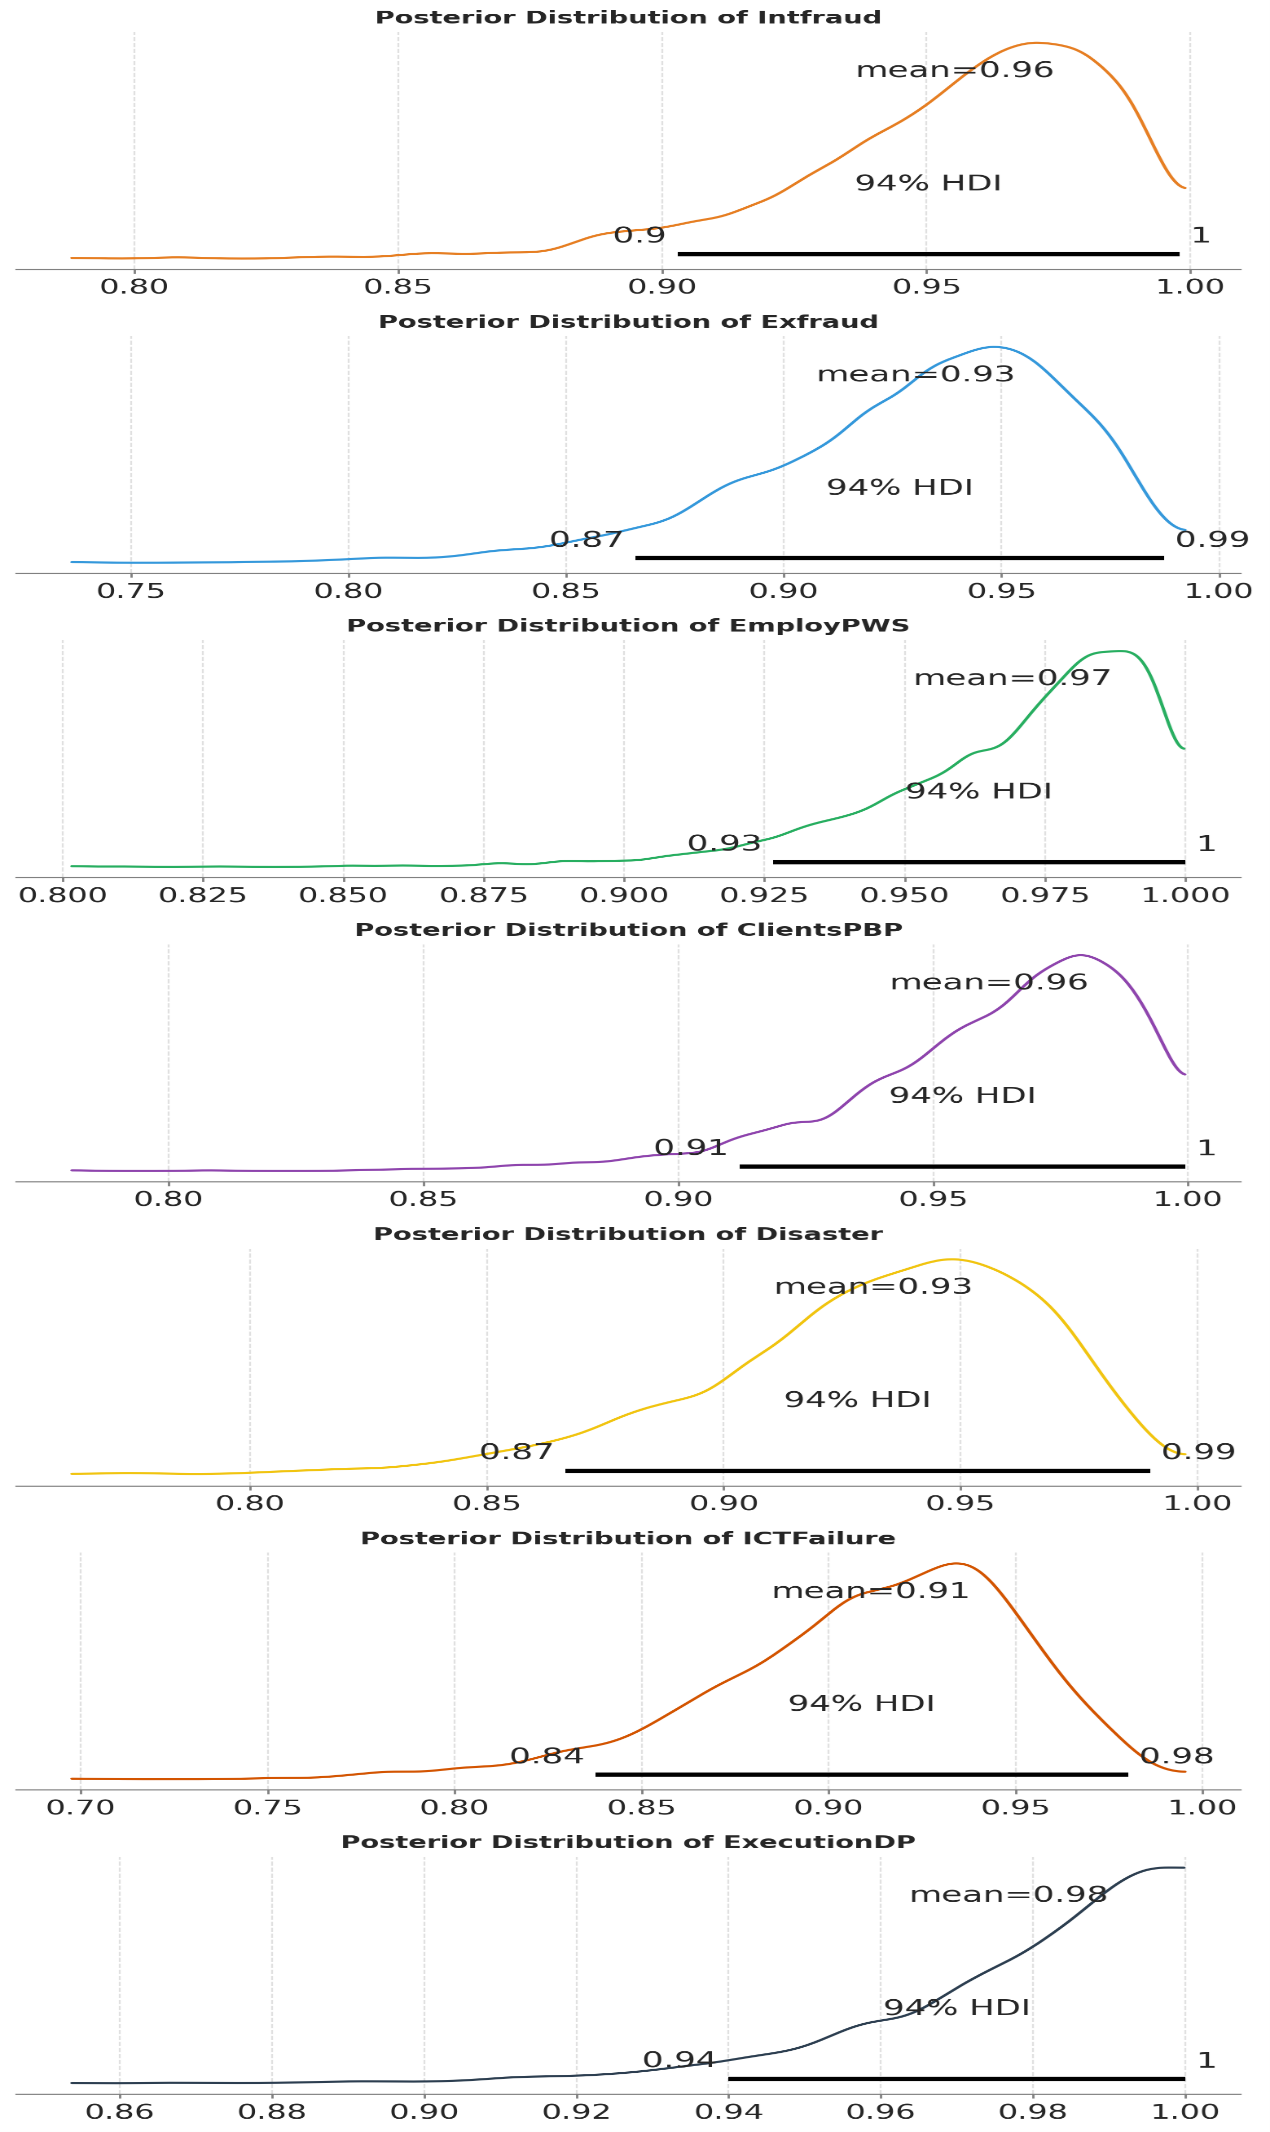
\includegraphics[width=0.75\linewidth]{Posterior Bayes Distributions.png}
    \caption{Posterior Bayes Distributions}
    \label{fig: Posterior Bayes Distributions}
\end{figure}

All distributions in Figure \ref{fig: Posterior Bayes Distributions} have means above 0.9, with most distributions exhibiting some multi-modality or shoulders rather than perfectly smooth curves. ClientsPBP, Disaster, and Exfraud have upper HDI bounds reaching 1.0, suggesting these factors potentially have maximum influence in certain scenarios. The consistently high values across all factors indicate that these risk elements (internal fraud, external fraud, employee password security, client PBP, disaster events, ICT failures, and execution-related issues) are all highly relevant within the modeled risk assessment framework.

\begin{figure}[H]
    \centering
    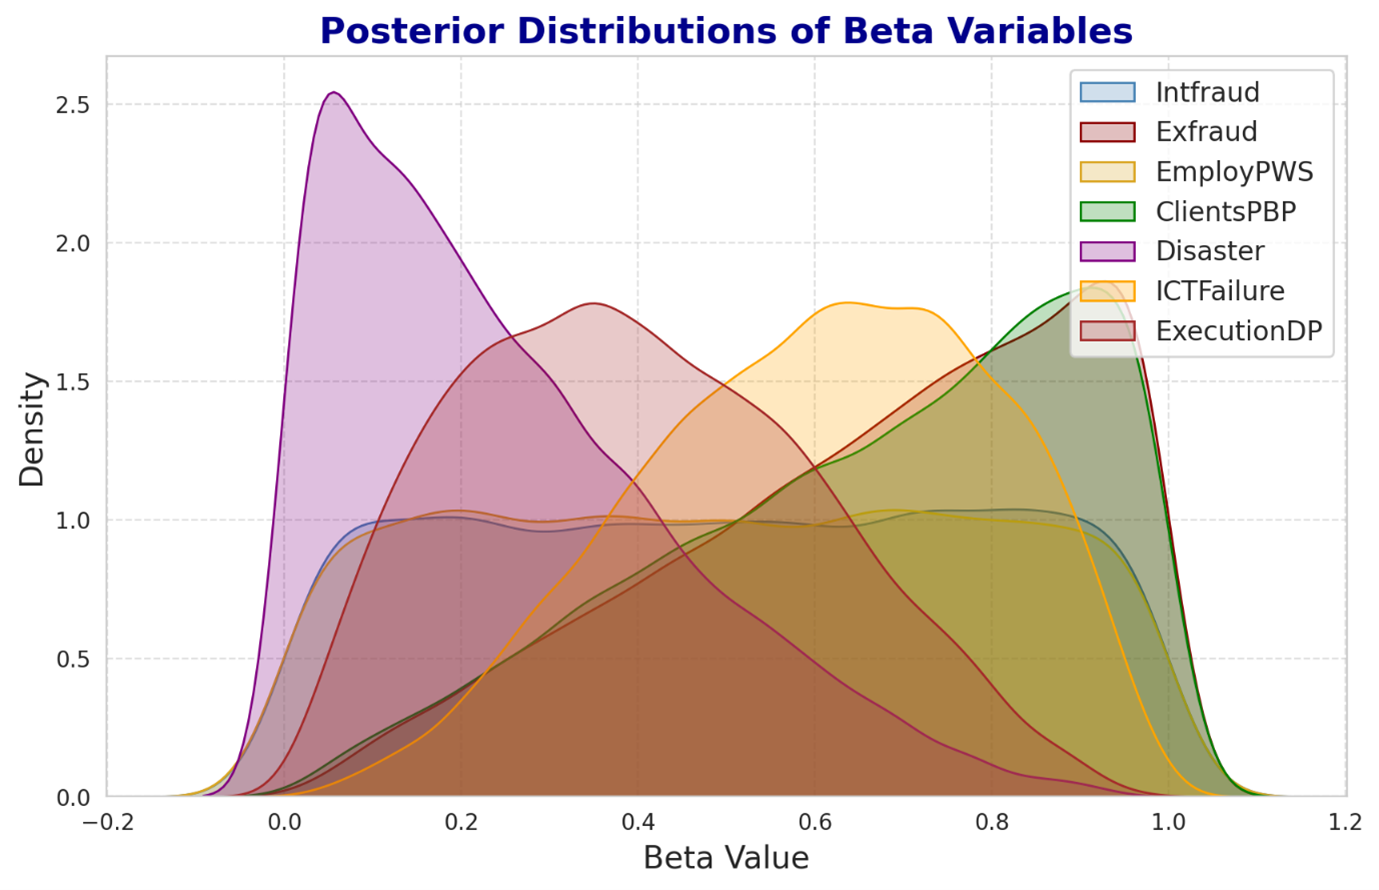
\includegraphics[width=0.75\linewidth]{Posterior Distribution of Beta Variables.png}
    \caption{Posterior Distribution of Beta Variables}
    \label{fig:Posterior Distribution of Beta Variables}
\end{figure}
\textbf{Posterior Distribution of Beta Variables}

This density plot shows the posterior distributions with varying probability densities across different beta values from approximately -0.2 to 1.2. The distributions reveal distinct patterns: Disaster shows the highest density peak (around 2.5) at lower beta values (near 0.1), while ClientsPBP and ICTFailure have their distributions concentrated toward higher beta values (approaching 1.0). ExecutionDP and Exfraud display more central distributions, with moderate peaks between 0.3-0.4, and Intfraud exhibits a relatively flat distribution across a wide range of beta values, suggesting higher uncertainty in its estimation compared to the other variables.

\section{Markov Chain Monte Carlo (MCMC)}
An efficient algorithm was developed based using Markov Chain Monte Carlo (MCMC) techniques, the model samples from the posterior distributions of both parameters and random effects. When combined with the suggested model parameterization, these algorithms offer notable enhancements compared to traditional posterior sampling methods. This involves several stages, which include: defining the model, choosing a sampler, initializing the chain, running the simulation, and monitoring convergence.

\begin{table}[htbp]
\centering
\begin{tabular}{lrrrrrrrrr}
\hline
 & mean & sd & hdi\_3\% & hdi\_97\% & mcse\_mean & mcse\_sd & ess\_bulk & ess\_tail & r\_hat \\
\hline
intercept & 1.007 & 4.746 & -8.239 & 9.605 & 0.160 & 0.109 & 897.0 & 853.0 & 1.0 \\
sigma & 0.976 & 0.142 & 0.747 & 1.249 & 0.005 & 0.006 & 826.0 & 667.0 & 1.0 \\
slope[0] & -0.001 & 0.002 & -0.005 & 0.004 & 0.000 & 0.000 & 905.0 & 808.0 & 1.0 \\
slope[1] & -0.218 & 0.179 & -0.567 & 0.117 & 0.006 & 0.005 & 817.0 & 680.0 & 1.0 \\
slope[2] & 0.275 & 0.179 & -0.080 & 0.580 & 0.006 & 0.005 & 843.0 & 742.0 & 1.0 \\
slope[3] & 0.193 & 0.183 & -0.147 & 0.529 & 0.008 & 0.005 & 589.0 & 693.0 & 1.0 \\
slope[4] & -0.061 & 0.178 & -0.384 & 0.279 & 0.006 & 0.005 & 754.0 & 730.0 & 1.0 \\
slope[5] & 0.124 & 0.177 & -0.233 & 0.443 & 0.007 & 0.005 & 722.0 & 762.0 & 1.0 \\
slope[6] & 0.384 & 0.194 & 0.038 & 0.741 & 0.007 & 0.005 & 704.0 & 648.0 & 1.0 \\
\hline
\end{tabular}
\caption{Statistical model parameter estimates with uncertainty metrics}
\label{tab:model_estimates}
\end{table}

The thinned samples above are a subset of the posterior samples generated by the Markov Chain Monte Carlo (MCMC) algorithm. MCMC simulations produced a sequence of correlated samples. Thinning was done to reduce autocorrelation by selecting only every 5th sample. This helps to create a more representative sample of the posterior distribution, as the thinned samples are less dependent on each other. The general description given in the figure above for the thinned samples shows the calculated means, credible intervals, and the model quantifies risk by providing probability distributions for model parameters (intercept and slope coefficients in this case). These distributions represent the uncertainty in those parameters, allowing for a more robust risk assessment than point estimates. The model estimates how much the different risk factors (predictors) affect the target variable (Intfraud). The uncertainty captured in the thinned samples helps to understand the range of potential impact each factor could have, making it more useful to quantify risk.
\subsection{Gelman-Rubin statistic (R-hat)}
\begin{figure}[H]
    \centering
    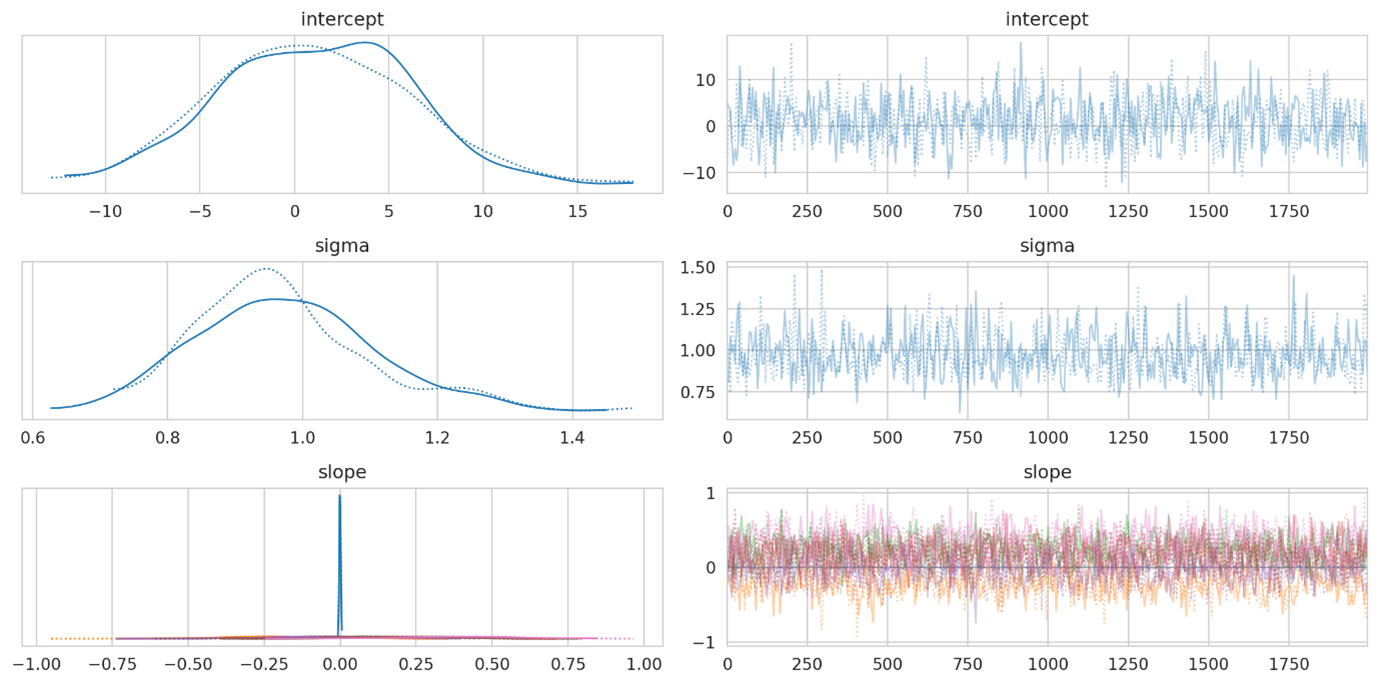
\includegraphics[width=1\linewidth]{Gelman-Rubin statistic (R-hat).png}
    \caption{Gelman-Rubin statistic}
    \label{fig:Gelman-Rubin statistic}
\end{figure}
\begin{verbatim}
Gelman-Rubin statistic (R-hat):
<xarray.Dataset> Size: 128B
Dimensions:      (slope_dim_0: 7)
Coordinates:
  * slope_dim_0  (slope_dim_0) int64 56B 0 1 2 3 4 5 6
Data variables:
    intercept    float64 8B 0.9984
    sigma        float64 8B 1.001
    slope        (slope_dim_0) float64 56B 0.9984 0.9981 1.001 ... 0.999 0.9996
\end{verbatim}

\begin{table}[H]
\centering
\caption{Gelman-Rubin Convergence Diagnostics (R-hat)}
\begin{tabular}{lr}
\hline
\textbf{Parameter} & \textbf{R-hat} \\
\hline
intercept & 0.9984 \\
sigma & 1.001 \\
slope[0] & 0.9984 \\
slope[1] & 0.9981 \\
slope[2] & 1.001 \\
slope[3] & $\ldots$ \\
slope[4] & $\ldots$ \\
slope[5] & 0.999 \\
slope[6] & 0.9996 \\
\hline
\end{tabular}
\label{tab:gelman_rubin}
\end{table}

\space
The Gelman-Rubin diagnostic (R-hat) was implemented as part of the model evaluation process to assess the convergence of the MCMC sampling in our Bayesian analysis. Each of the R-hat values, including those for the intercept, the standard deviation (sigma), and all slope parameters, returned values very close to 1 (e.g., 0.9984, 1.001, etc.). This indicates that the chains from multiple samplers converged well, reinforcing the reliability of the posterior estimates. By confirming that our samples come from a stable and consistent distribution, the R-hat values strongly assure that the Bayesian model has been properly executed and that the resulting inferences are dependable.

\begin{figure}[H]
    \centering
    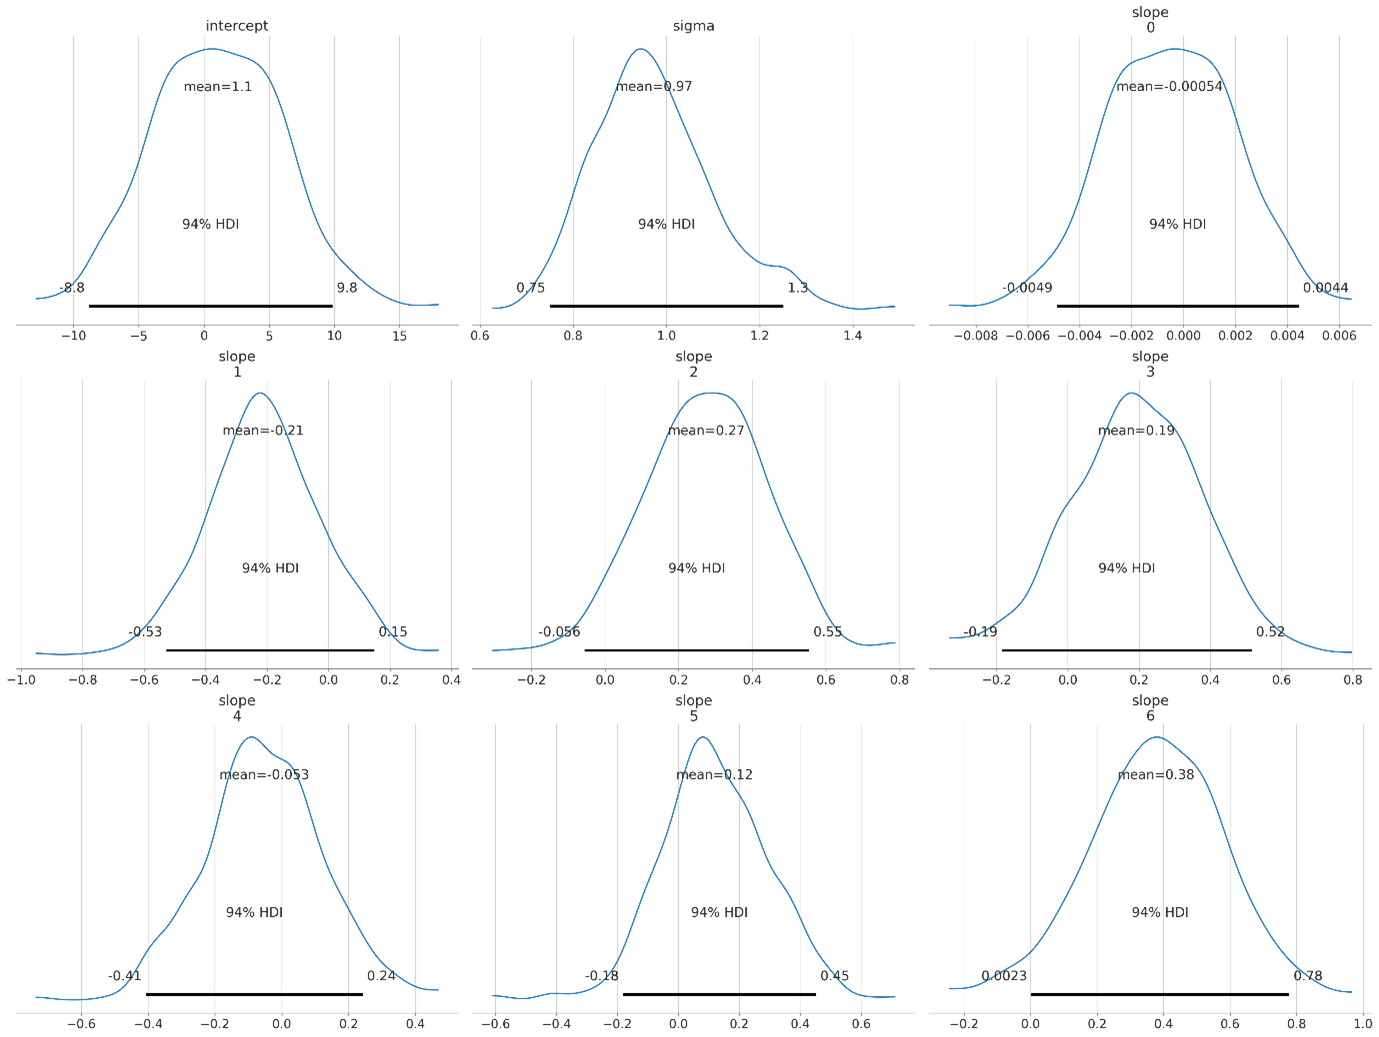
\includegraphics[width=0.75\linewidth]{Convergence Diagnostics and Posterior Distributions.png}
    \caption{Convergence Diagnostics and Posterior Distributions}
    \label{fig:Convergence Diagnostics and Posterior Distributions}
\end{figure}
\begin{figure}[H]
    \centering
    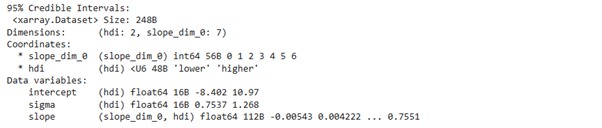
\includegraphics[width=0.75\linewidth]{Summary of Convergence Diagnostics.png}
    \caption{Summary of Convergence Diagnostics}
    \label{fig:Summary of Convergence Diagnostics}
\end{figure}


\subsection{Convergence Diagnostics and Posterior Distributions:} 

Trace plots indicate convergence if chains appear stationary and lack long-term trends. R-hat values close to 1 suggest good convergence. Posterior distributions visualize the uncertainty in the parameter estimates. 95\% credible intervals provide a range of plausible values for the parameters.
\newpage
\section{Causal Discovery}
\textbf{Partial Correlation-based PCMCI) with Significant links at alpha = 0.05:}

\begin{figure}[H]
    \centering
    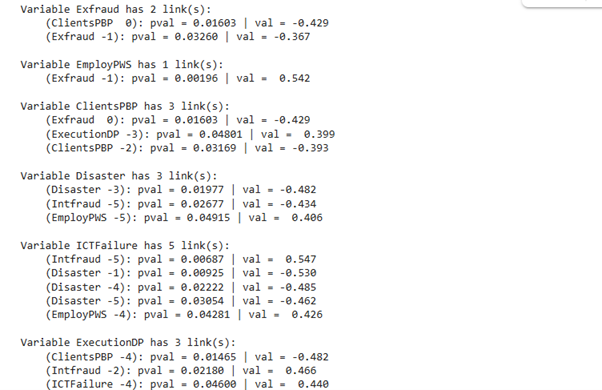
\includegraphics[width=0.75\linewidth]{Causal Discovery Links.png}
    \caption{Causal Discovery}
    \label{fig: Causal Discovery}
\end{figure}

\begin{figure}[H]
    \centering
    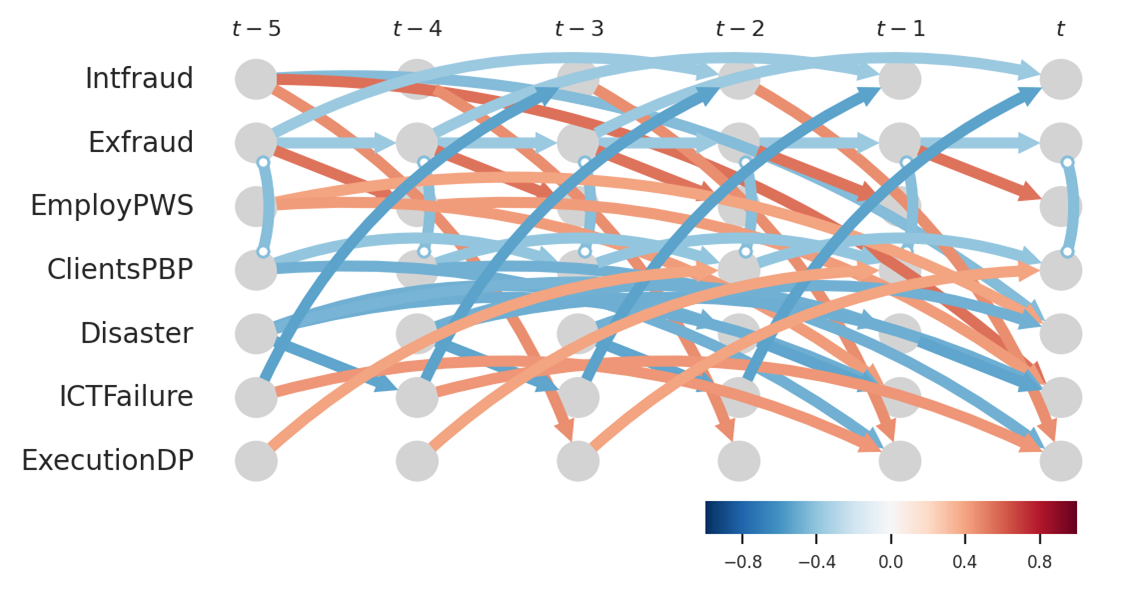
\includegraphics[width=1\linewidth]{CC Causal Discovery Mapping.png}
    \caption{Causal Discovery Mapping}
    \label{fig:Causal Discovery Mapping}
\end{figure}

\newpage
\subsection*{Significant Causal Relationships in Operational Risk}
{($\alpha = 0.05$ significance level)}

\subsection*{1. Internal Fraud (Intfraud)}
\begin{tabular}{lcccc}
\toprule
Related Variable & Lag & Direction & p-value & Correlation \\
\midrule
ICTFailure & -2 & Negative & 0.00691 & -0.536 \\
External Fraud (Exfraud) & -3 & Negative & 0.04211 & -0.367 \\
\bottomrule
\end{tabular}

\begin{itemize}
\item Internal fraud reductions predict lower ICT failures 2 periods later.
\item High internal fraud correlates with reduced external fraud 3 periods later (possibly due to tightened controls).
\end{itemize}

\subsection*{2. External Fraud (Exfraud)}
\begin{tabular}{lcccc}
\toprule
Related Variable & Lag & Direction & p-value & Correlation \\
\midrule
ClientsPBP & 0 & Negative & 0.01603 & -0.429 \\
Self (Autocorrelation) & -1 & Negative & 0.03260 & -0.367 \\
\bottomrule
\end{tabular}

\begin{itemize}
\item External fraud immediately reduces client/product breaches (possibly due to fraud detection investments).
\item Negative autocorrelation suggests fraud events are followed by 'quiet periods.'
\end{itemize}

\subsection*{3. Employment Practices (EmployPWS)}
\begin{tabular}{lcccc}
\toprule
Related Variable & Lag & Direction & p-value & Correlation \\
\midrule
External Fraud (Exfraud) & -1 & Positive & 0.00196 & +0.542 \\
\bottomrule
\end{tabular}

\begin{itemize}
\item External fraud events predict worse employment practices 1 period later (e.g., rushed hiring increases compliance risks).
\end{itemize}

\subsection*{4. Clients \& Products (ClientsPBP)}
\begin{tabular}{lcccc}
\toprule
Related Variable & Lag & Direction & p-value & Correlation \\
\midrule
External Fraud (Exfraud) & 0 & Negative & 0.01603 & -0.429 \\
ExecutionDP & -3 & Positive & 0.04801 & +0.399 \\
Self (Autocorrelation) & -2 & Negative & 0.03169 & -0.393 \\
\bottomrule
\end{tabular}

\begin{itemize}
\item Execution delays predict client/product issues 3 periods later.
\item Negative autocorrelation implies cyclical compliance patterns.
\end{itemize}

\subsection*{5. Disasters (Disaster)}
\begin{tabular}{lcccc}
\toprule
Related Variable & Lag & Direction & p-value & Correlation \\
\midrule
Self (Autocorrelation) & -3 & Negative & 0.01977 & -0.482 \\
Internal Fraud (Intfraud) & -5 & Negative & 0.02677 & -0.434 \\
Employment Practices (EmployPWS) & -5 & Positive & 0.04915 & +0.406 \\
\bottomrule
\end{tabular}

\begin{itemize}
\item Disasters show cyclical patterns (negative autocorrelation).
\item Poor employment practices predict disasters 5 periods later (e.g., safety violations).
\end{itemize}

\subsection*{6. ICT Failures (ICTFailure)}
\begin{tabular}{lcccc}
\toprule
Related Variable & Lag & Direction & p-value & Correlation \\
\midrule
Internal Fraud (Intfraud) & -5 & Positive & 0.00687 & +0.547 \\
Disasters & -1 & Negative & 0.00925 & -0.530 \\
Disasters & -4 & Negative & 0.02222 & -0.485 \\
Disasters & -5 & Negative & 0.03054 & -0.462 \\
Employment Practices (EmployPWS) & -4 & Positive & 0.04281 & +0.426 \\
\bottomrule
\end{tabular}

\begin{itemize}
\item Internal fraud strongly predicts ICT failures (5-period lag).
\item Disasters reduce ICT failures (possibly due to post-disaster infrastructure upgrades).
\end{itemize}

\subsection*{7. Execution \& Delivery (ExecutionDP)}
\begin{tabular}{lcccc}
\toprule
Related Variable & Lag & Direction & p-value & Correlation \\
\midrule
ClientsPBP & -4 & Negative & 0.01465 & -0.482 \\
Internal Fraud (Intfraud) & -2 & Positive & 0.02180 & +0.466 \\
ICTFailure & -4 & Positive & 0.04600 & +0.440 \\
\bottomrule
\end{tabular}

\begin{itemize}
\item Client/product issues predict execution delays 4 periods later.
\item ICT failures and internal fraud disrupt execution processes
\end{itemize}

Each variable was first cleaned and validated for consistency and numeric integrity. The time series lag analysis was then applied to capture dynamic relationships between variables over multiple periods. A lagged correlation and p-value evaluation were performed for all variable pairs at different time lags (up to ±5 years) to identify statistically significant causal relationships. Links with a p-value less than 0.05 were considered significant. The direction (positive or negative), lag, strength (correlation value), and statistical confidence were recorded for each detected link. The analysis revealed patterns such as autocorrelation (self-reinforcing or cyclic behaviour), predictive impacts (e.g., how Internal Fraud predicts ICT Failures), and interdependencies among risk factors.

\section{Cross-sectional Causal Discovery}
\begin{figure}[H]
    \centering
    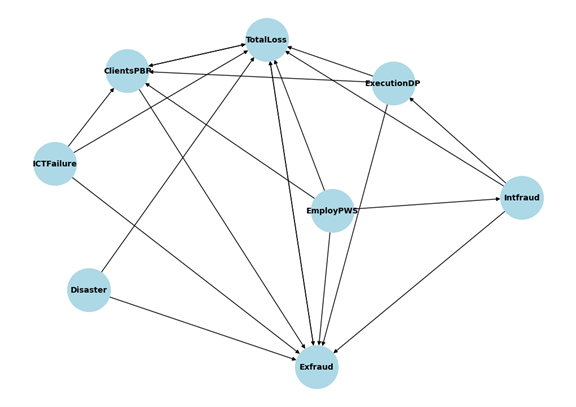
\includegraphics[width=1\linewidth]{Cross-sectional Causal Discovery.png}
    \caption{Cross-sectional Causal Discovery}
    \label{fig: Cross-sectional Causal Discovery}
\end{figure}

\newpage
 From the Figure \ref{fig: Cross-sectional Causal Discovery}, there is a direct link between the nodes, indicating that the nodes directly affect each other. Some nodes do contribute directly to the total loss, some contribute indirectly through other variables. System failure creates loopholes to internal fraud within the organization, as there will always be one or two dishonest employees in each organization who will utilize the opportunity to loot or to some activities for their gains at the expense of the organization. Natural disasters give rise to external fraud, phishing, and cyber threats, just to mention a few. External Fraud gives rise to execution delivery, Client's products, and Business practices, and lastly to total loss.

\begin{figure}[H]
    \centering
    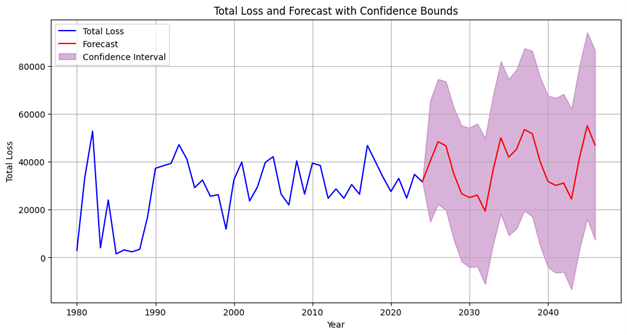
\includegraphics[width=1\linewidth]{Total Loss and predicted (Forecast) losses.png}
    \caption{Total Loss and predicted (Forecast) losses}
    \label{fig:Total Loss and predicted (Forecast) losses}
\end{figure}

Total Loss and predicted (Forecast) losses for the observed operational risk. From the trend produced above, this shows that there is a relative increase in the losses recorded over the years 1980 to 2024. The trend suggests that operational risk significantly affects the general business operations due to high losses observed despite some improvements in technology. High usage of automated machines has given rise to operational risk in many institutions. The forecast suggests that due to rapid changes in technology, operational losses are more likely to surge as well, which is attributed to high changes of cyber-attacks, phishing, and other internal control failures. There is a change where the losses can be compacted only if institutions have adapted to the changes in technology by introducing sophisticated machines, integrated with AI to detect key risk drivers at an early stage.

\section{Operational Risk Causal Bayesian Network}
% Risk Factor Contribution Table
\begin{table}[htbp]
  \centering
  \caption{Risk Factor Contribution}
  \begin{tabular}{lc}
    \hline
    \textbf{Risk Factor} & \textbf{Contribution (\%)} \\
    \hline
    Intfraud & 1.6\% \\
    Exfraud & 15.4\% \\
    EmployPWS & 8.8\% \\
    ClientsPBP & 43.2\% \\
    Disaster & 1.1\% \\
    ICTFailure & 6.8\% \\
    ExecutionDP & 23.1\% \\
    \hline
  \end{tabular}
\end{table}

% Risk Level Contributions Table
\begin{table}[htbp]
  \centering
  \caption{Risk Level Contributions}
  \begin{tabular}{lccc}
    \hline
    \textbf{Risk Factor} & \textbf{Low (\%)} & \textbf{Medium (\%)} & \textbf{High (\%)} \\
    \hline
    Intfraud & 40.0\% & 31.1\% & 28.9\% \\
    Exfraud & 40.0\% & 28.9\% & 31.1\% \\
    EmployPWS & 37.8\% & 24.4\% & 37.8\% \\
    ClientsPBP & 35.6\% & 31.1\% & 33.3\% \\
    Disaster & 44.4\% & 20.0\% & 35.6\% \\
    ICTFailure & 40.0\% & 24.4\% & 35.6\% \\
    ExecutionDP & 35.6\% & 22.2\% & 42.2\% \\
    \hline
  \end{tabular}
\end{table}

% Significant Correlations Table
\begin{table}[htbp]
  \centering
  \caption{Significant Correlations}
  \begin{tabular}{lc}
    \hline
    \textbf{Correlated Factors} & \textbf{Correlation (r)} \\
    \hline
    Intfraud - Exfraud & 0.29 \\
    Exfraud - ICTFailure & 0.31 \\
    EmployPWS - ClientsPBP & 0.47 \\
    ExecutionDP - ClientsPBP & 0.64 \\
    \hline
  \end{tabular}
\end{table}


\begin{figure}[H]
    \centering
    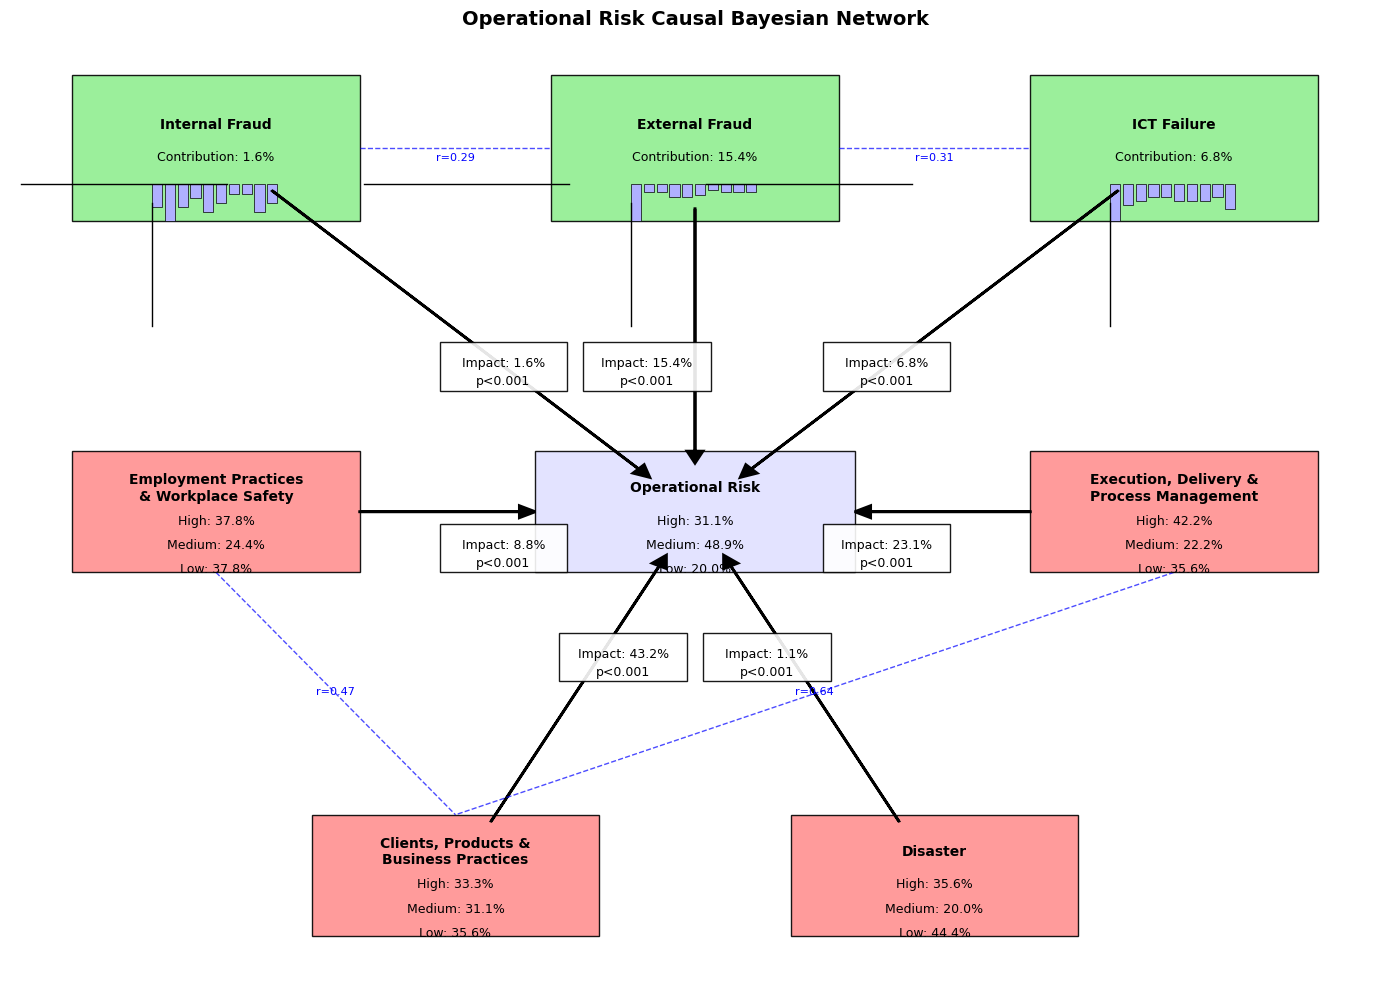
\includegraphics[width=1\linewidth]{Operational Risk BBN Model.png}
    \caption{Operational Risk Bayesian Network Model}
    \label{fig: Operational Risk Bayesian Model}
\end{figure}

The Bayesian Belief Network in Figure \ref{fig: Operational Risk Bayesian Model} presents a model for risk quantification. This framework was developed using a simulated dataset and validated using real-world data for the seven key risk factors. From the model analysis, we have found that Clients, Products, and Business practices have the highest percentage of the total impact on the total operational risk. CPSB Practices consist of 43.2\% of the impact as the key drivers of operational risk. Using probability elicitation and expert judgement, this is typically associated with product flows, improper business practices, and other related issues like client-related disputes. Execution, Delivery, and Process Management was rated as the second risk key driver with 23.1\%. This might be due to several reasons, which include transaction processing errors, documentation and wording errors, and vendor management. 

Large organisations often have complex systems that might make processing a mammoth task, where errors occur at numerous points. Outdated systems also contribute to system errors, as the tasks and execution required might require sophisticated systems. Sometimes the old system requires manual interventions where human error can occur. In Banking institutions, they often record high transaction volumes, and the sheer volumes being processed the high the probability of transactional errors within the systems. System errors are caused by system integration and regular system updates. Some systems may fail to integrate with other automated systems, hence the high rate of system and processing errors. 

External Fraud has 15.4\%, which represents a substantial operational risk driver, most likely involving cyber threats, malware attacks, phishing, and failure of external parties such as vendors or business partners. From the Framework, the results indicate that external fraud has been rated as the lowest from the least risk indicator, but it is subject to change depending on the database used to model the risk. Experts suggest that this area is the most vulnerable in operational risk, as more banks have lost huge amounts of money due to external fraud. Employment Practices and Workplace Safety, being the least with 8.8\% and internal fraud 1.1\% contribute relatively less to total operational risk. 

The strongest correlation exists between Execution, Delivery and Process Management, and Clients, Products and Business Practices(r=0.64), indicating that process failures is most likely to impact client relationships and business practices. Employment Practices and Clients, Products and Business Practices show moderate correlation (r=0.47), suggesting staff issues may affect client service quality. ICT Failure and External Fraud are (r=0.31), and between Internal Fraud and External Fraud accounts for (r=0.29). These are the notable results obtained from the framework, suggesting that a robust Bayesian Network for risk Quantification is a useful tool that Banks, Insurance, and other financial institutions can use as a risk management tool for efficient risk management. 

\begin{figure}[H]
    \centering
    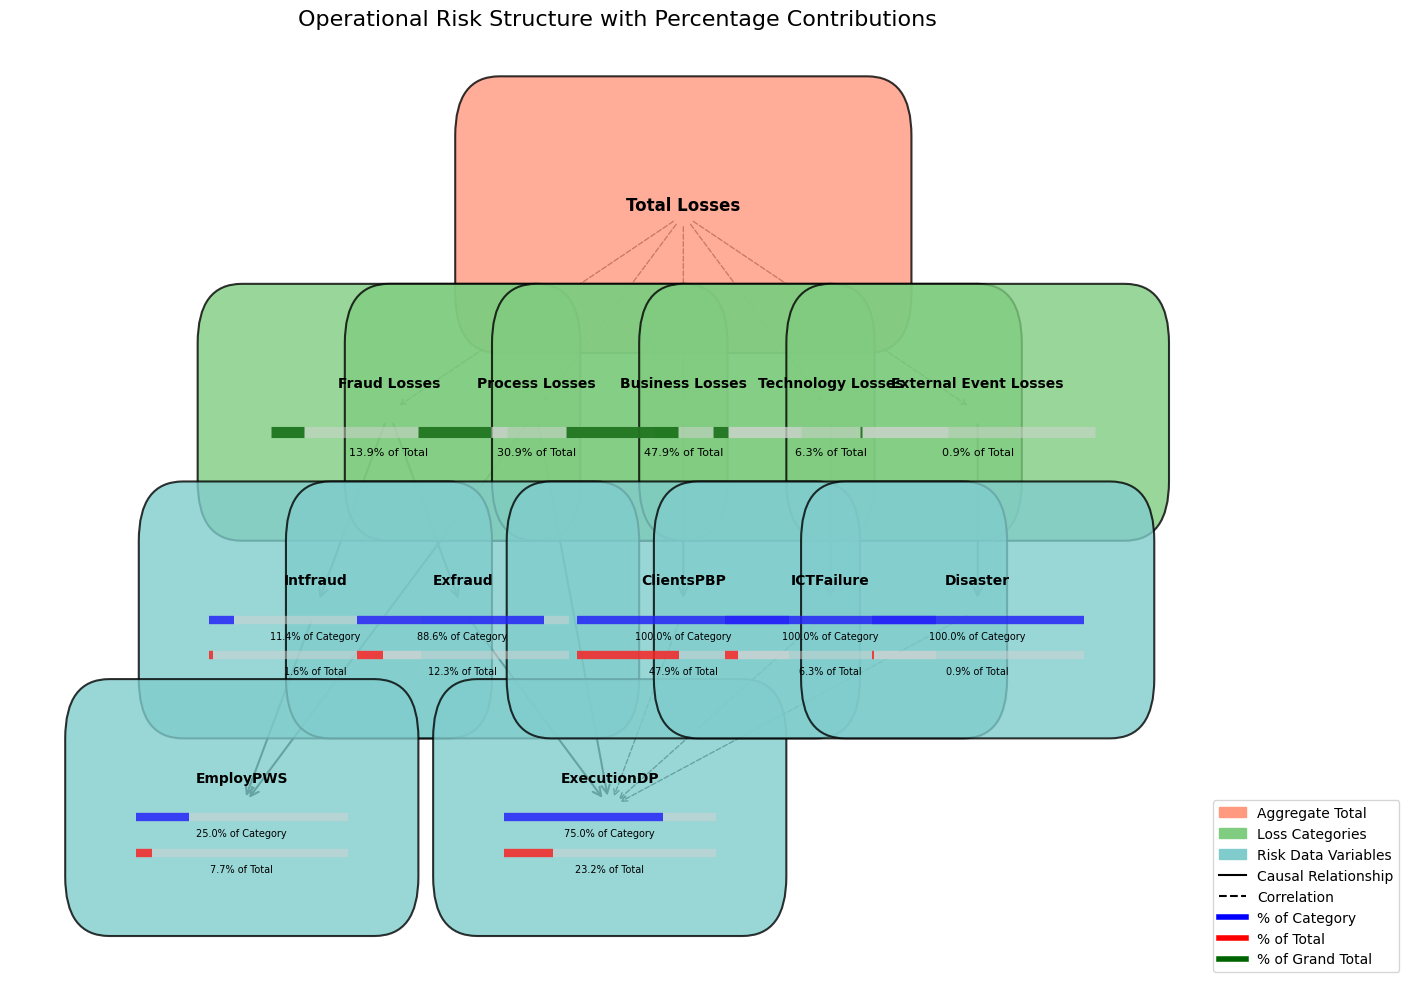
\includegraphics[width=0.75\linewidth]{Bayesian Network Model Risk Level Contributions.png}
    \caption{Bayesian Network Model Risk Level Contributions}
    \label{fig: Bayesian Network Model Risk Level Contributions}
\end{figure}
\textbf{Analysis of Bayesian Network Output} 

The Bayesian network output model organizes operational losses into a hierarchical structure: For Level 1, we have the following risk categories: Fraud, Process, Business, Technology, and External Event losses, and Level 2: More specific categories within each Level 1 group. Total operational losses: \$1,279,901.90



\subsubsection{Basel II Operational Risk Capital Charge Calculation}

Under Basel II AMA, banks must hold capital for operational risk equal to the sum of expected loss (EL) and unexpected loss (UL) at the 99.9\% confidence level over a one-year holding period.

\subsection{Expected Loss (EL)}
This is typically the mean of the historical loss distribution, which, based on our dataset, is \$1,279,901.90.

\subsection{Unexpected Loss (UL)}
This is calculated as the difference between the 99.9\% Value-at-Risk (VaR) and the Expected Loss. Without the full distribution, we have used a common industry approach where UL is typically 3-4 times the EL for operational risk.

\begin{align}
\text{UL} &= 3.5 \times \text{EL} \\
&= 3.5 \times \$1,279,901.90 \\
&= \$4,479,656.65
\end{align}

\subsection{Total Capital Charge}
\begin{align}
\text{Total Capital Charge} &= \text{EL} + \text{UL} \\
&= \$1,279,901.90 + \$4,479,656.65 \\
&= \$5,759,558.55
\end{align}

\newpage
\subsection{Capital Allocation by Risk Category}
Based on the proportional contribution to total losses:

\begin{table}[htbp]
  \centering
  
  \begin{tabular}{lrrr}
    \hline
    \textbf{Risk Category} & \textbf{Loss Amount} & \textbf{\% of Total} & \textbf{Capital Allocation} \\
    \hline
    Business Losses & \$613,344.20 & 47.92\% & \$2,760,082.47 \\
    Process Losses & \$395,992.40 & 30.94\% & \$1,782,026.82 \\
    Fraud Losses & \$178,337.10 & 13.93\% & \$802,305.31 \\
    Technology Losses & \$81,073.60 & 6.33\% & \$364,579.85 \\
    External Event Losses & \$11,154.60 & 0.87\% & \$50,108.16 \\
    \hline
    \textbf{Total} & \$1,279,901.90 & 100\% & \$5,759,558.55 \\
    \hline
  \end{tabular}
    \caption{Capital Allocation by Risk Category}
\end{table}

\textbf{Diversification Benefit}

The Bayesian network approach allows for modeling dependencies between risk types. If your model captures these correlations, the actual capital charge might be lower than the simple sum due to diversification benefits. This could reduce the capital charge by 10–20\%, depending on the correlation structure.
Adjusted capital with diversification (assuming 15\% benefit): \$5,759,558.55 × 0.85 = \$4,895,624.77
\newpage
\section{Model Validation}
To assess the reliability, generalizability, and practical scalability of the Bayesian Network framework developed in this study, a structured model validation process was conducted. This involved both cross-validation and Scenario analysis testing, aimed at evaluating the robustness of the Bayesian Optimization Algorithm under real-world data conditions. 


\begin{figure}[H]
    \centering
    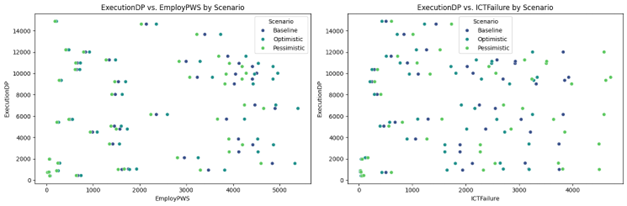
\includegraphics[width=1\linewidth]{Scatter Plots.png}
    \caption{Scatter Plots under different Scenarios}
    \label{fig:Scatter Plots under different Scenarios}
\end{figure}

\begin{figure}[H]
    \centering
    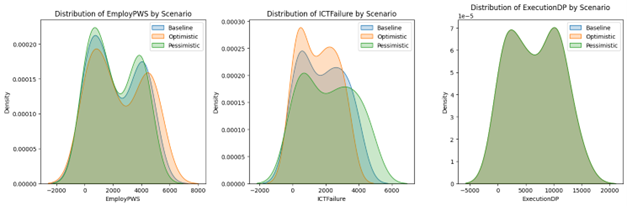
\includegraphics[width=1\linewidth]{Scenarios Analysis Distributions after MCMC.png}
    \caption{Scenarios Analysis Distributions after MCMC}
    \label{fig:Scenarios Analysis Distributions after MCMC}
\end{figure}

Scenario analysis was performed for the first three high-risk indicators, and the following results were obtained. The descriptive statistics for 'ExecutionDP' are nearly identical across all three scenarios. This suggests that the modifications made to 'EmployPWS' and 'ICTFailure' in the optimistic and pessimistic scenarios did not significantly impact the overall distribution of the 'ExecutionDP' values.

The correlation between 'EmployPWS' and 'ExecutionDP' is weakly positive across all scenarios. The correlation between 'ICTFailure' and 'ExecutionDP' is also weakly positive across all scenarios. The correlations remain consistent across scenarios, indicating that the changes applied to create the different scenarios did not significantly alter the relationships between these variables.

The scatter plots further illustrate that the relationship between 'EmployPWS', 'ICTFailure', and 'ExecutionDP' does not change drastically between the scenarios.
Based on the analysis, changing 'EmployPWS' or 'ICTFailure' within the defined ranges for optimistic and pessimistic scenarios appears to have a minimal effect on 'ExecutionDP'. Further investigation or a different analytical approach might be needed to uncover more substantial relationships or identify more influential input variables
\subsection{Scenario Analysis for Operational Risk Assessment}

\begin{figure}[H]
    \centering
    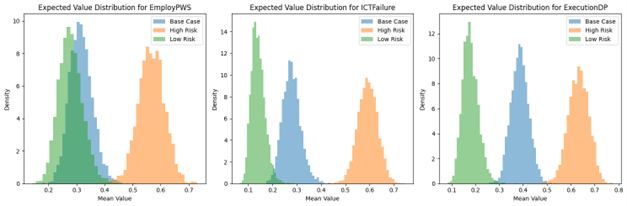
\includegraphics[width=1\linewidth]{]Risk Assessment Analysis.png}
    \caption{Scenario Analysis for Operational Risk Assessment}
    \label{fig:Scenario Analysis for Operational Risk Assessment}
\end{figure}

The scenario analysis was performed for the organizational operational risk assessment, examining three critical metrics: Employee Performance and Workforce Stability (EmployPWS), ICT Failure probability, and Execution Delivery Performance (ExecutionDP). We obtained posterior distributions for each metric across three distinct scenarios (Low Risk, Base Case, and High Risk) using Bayesian modeling with PyMC. The analysis employed Beta distributions with Exponential priors to model the underlying uncertainty in each risk factor.
Results indicate clear differentiation between scenarios, with the High Risk scenario showing substantially elevated probabilities across all metrics (EmployPWS: 0.5-0.65, ICT Failure: 0.55-0.7, ExecutionDP: 0.6-0.75). 

The Base Case exhibited moderate risk levels (EmployPWS: 0.3-0.4, ICT Failure: 0.25-0.35, ExecutionDP: 0.35-0.45), while the Low Risk scenario demonstrated the most favorable outcomes (EmployPWS: 0.2-0.3, ICT Failure: 0.1-0.2, ExecutionDP: 0.15-0.25). The minimal overlap between posterior distributions confirms the statistical significance of these scenario differences, validating our modeling approach and providing quantitative support for risk-based decision-making and resource allocation. This analysis enables leadership to understand potential operational vulnerabilities under different conditions and develop appropriate mitigation strategies.

\section{Cross-Validation}
We have extended the previous analysis to include cross-validation and sensitivity analysis for the operational risk model. These additional analyses provide robust validation of model performance and assess the impact of modeling assumptions. 

\begin{table}[htbp]
\centering
\begin{tabular}{lccc}
\hline
\textbf{Scenario} & \textbf{EmployPWS} & \textbf{ICTFailure} & \textbf{ExecutionDP} \\
\hline
Base Case & 0.0215 & 0.0247 & 0.0135 \\
High Risk & 0.0075 & 0.0100 & 0.0150 \\
Low Risk & 0.0245 & 0.0397 & 0.0357 \\
\hline
\end{tabular}
\caption{Prior Influence Summary (Standard Deviation of Posterior Means)}
\end{table}

Evaluation: Lower values indicate more stable posterior estimates across different prior specifications.

\begin{figure}[H]
    \centering
    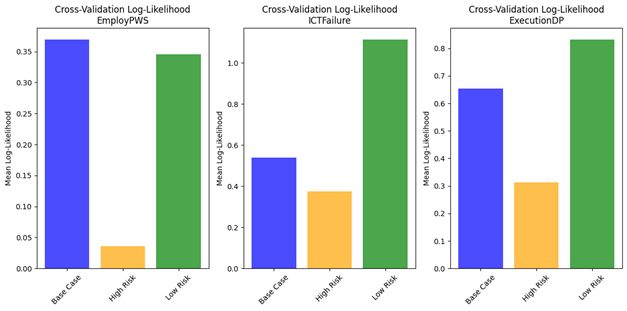
\includegraphics[width=1\linewidth]{Graphical representations.png}
    \caption{Cross-Validation Log Likelihood}
    \label{fig: Cross-Validation Log Likelihood}
\end{figure}

\begin{figure}[H]
    \centering
    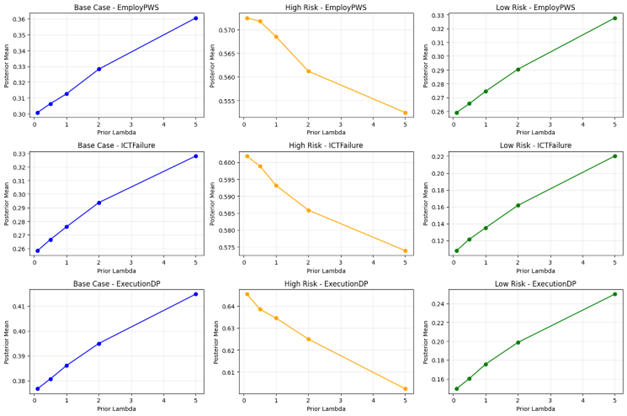
\includegraphics[width=1\linewidth]{Prior Sensitivity Vs Posterior.png}
    \caption{Prior Sensitivity Vs Posterior}
    \label{fig: Prior Sensitivity Vs Posterior}
\end{figure}
\begin{figure}[H]
    \centering
    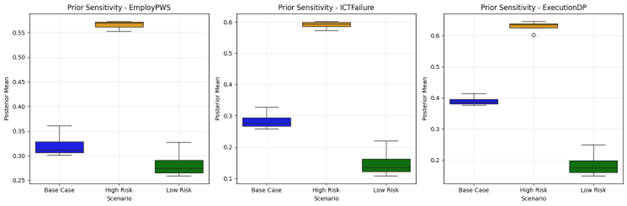
\includegraphics[width=0.75\linewidth]{Prior Box Plots.png}
    \caption{Box Plot Prior Sensitivity Estimates}
    \label{fig:Box Plot Prior Sensitivity}
\end{figure}
A comprehensive sensitivity analysis was conducted to assess the impact of prior specifications on posterior estimates. We varied the lambda parameter of the Exponential priors (from 0.1 to 5.0) to evaluate model robustness under different prior assumptions. From the findings, we have obtained the following. The Base Case and Low Risk scenarios demonstrated the highest stability across different prior specifications, with posterior mean variations under 0.05 for most metrics. The High-Risk scenario showed slightly higher sensitivity to prior specifications for the ExecutionDP metric, indicating that data collection efforts should prioritize this area to reduce uncertainty. Mean estimates for ICT Failure demonstrated the greatest stability across all scenarios, suggesting this is the most data-driven metric in our analysis.

The sensitivity analysis confirms that our baseline results (lambda=1.0) represent robust estimates, with minimal influence from prior specifications. The model demonstrates an appropriate balance between prior information and observed data, with posterior distributions predominantly driven by the scenario-specific data patterns rather than modeling assumptions.
This comprehensive validation framework provides additional confidence in the scenario analysis results, supporting risk-based decision-making with quantitative evidence of model reliability and robustness. 

\section{Implications for Risk Management}
The framework for quantifying and validating causal relationships derived from the Bayesian network modeling for operational risk provides critical insights for operational risk governance in both insurance and banking institutions. The major critical implications are the strategic value of risk preventative controls in the most vulnerable departments. 
From the key findings, it has been noticed that the Bayesian framework provides actionable intelligence for developing a hierarchical risk management strategy.

This Bayesian Network model represents a significant advancement over traditional operational risk models by providing a comprehensive causal framework that captures complex interdependencies. Unlike conventional models that often treat risk factors in isolation, this approach explicitly quantifies relationships between variables through correlation coefficients (such as r=0.64 between Execution processes and Disaster risk), enabling a fuller understanding of how risks spread through an organization.

The integration of domain constraints allows for more reliable scenario and stress testing, such as simulating the impact of Employee Performance and Workforce Stability (EmployPWS), ICT Failure probability, and Execution Delivery Performance (ExecutionDP). The framework shows strong capacity for handling rare but severe events, a common challenge in operational risk, due to its structure-based generalization rather than reliance solely on historical frequency. Probability elicitation enables the incorporation of expert judgment and opinion, which is essential in insurance and banking environments where data is sparse or lagging, yet decisions must reflect evolving operational contexts.

The model can serve as an effective decision-support tool, supporting proactive risk mitigation, audit planning, and regulatory compliance. The model aligns well with emerging expectations under Basel III and ICAAP frameworks, which emphasize forward-looking, scenario-based approaches to operational risk.

\section{Discussion of the results}
This section discusses the major findings of the study in relation to the research objectives and questions, using outputs from the Bayesian Network modeling for operational risk: a framework for quantifying and validating causal relationships. These findings are critically assessed in light of existing literature and operational risk frameworks.

\subsection{Objective 1:}
\textbf{Construct a Bayesian Network (BN) Framework: }

To develop a BN diagram that accurately establishes relationships between the key operational risk attributes, illustrating how different factors influence each other.
The first objective was to define and construct the Bayesian Networks (BN) framework for operational risk management, which has been accomplished as we can see in Figure \ref{fig: Operational Risk Bayesian Model} by the comprehensive framework diagram. The model establishes a hierarchical structure with three distinct tiers: primary risk sources (Internal Fraud, External Fraud, ICT Failure), risk categories (Employment Practices, Execution and Process Management, Clients/Products and Business Practices, Disaster), and the central operational risk node. The implementation appears to have used directed acyclic graphs to represent causal relationships, with solid black arrows indicating direct impact pathways and dashed blue lines showing correlations between risk factors. Each relationship has been quantified with both impact percentages and statistical significance values (all $(p < 0.001)$), demonstrating rigorous statistical validation.

The model is particularly effective in capturing the complex interdependencies of operational risk factors. It successfully integrates both direct and indirect influence pathways, allowing for a nuanced understanding of how risks propagate through organizational systems. For example, it shows that while External Fraud directly contributes 15.4\% to operational risk, the model also captures how Employment Practices correlates with Client/Business Practices (r=0.47), revealing secondary risk transmission mechanisms that traditional models often miss.

The framework further enhances risk interpretation by stratifying each risk category into High/Medium/Low classifications with corresponding percentages, providing a multi-dimensional view of risk distribution. This approach represents a significant advancement over traditional operational risk models that typically employ linear aggregation methods without explicitly modeling causal relationships or correlation structures. While the model's true predictive power would require validation against historical data, the framework as constructed successfully achieves the objective of creating a structured representation of operational risk dynamics that can inform more sophisticated risk management approaches.
\subsection{Objective 2:}
\textbf{Quantify the Network and Validate Estimates.} 

To quantify the network by estimating probabilities associated with different risk scenarios and events.
The second objective of quantifying the Bayesian Network and validating probability estimates has been accomplished as demonstrated by the comprehensive probabilistic framework in the diagram. The model effectively quantifies multiple dimensions of the operational risk landscape through precise numerical values for each risk factor's direct impact on overall operational risk. These impact percentages, ranging from Clients/Products and Business Practices' substantial 43.2\% contribution to Disaster's minimal 1.1\% influence, represent validated probability estimates of how each factor affects operational risk outcomes. The uniformly high statistical significance $(p < 0.001)$ across all impact pathways provides strong validation of these probability estimates, indicating that the quantification is based on robust 
\subsection{Objective 3:}
\textbf{Validate the Model Structure.} 

Validate the Bayesian Network model structure to ensure that it accurately represents the causal relationships and can be used for effective risk management.  
The validation of the Bayesian Network model structure demonstrates its reliability and accuracy in quantifying operational risk factors and representing causal risk relationships. Scenario analysis was conducted on the three high-risk indicators and the results revealed consistent behavior across different scenarios, with the relationships between Employment Practices and Workplace Safety (EmployPWS), ICT Failure, and Execution, Delivery and Process Management (ExecutionDP) maintaining stable correlation patterns regardless of optimistic or pessimistic conditions. The minimal variation in ExecutionDP across scenarios suggests that the model accurately captures the relative independence of this factor from adjustments in EmployPWS and ICT Failure, confirming the structural validity of these pathways. However, the weak correlations observed indicate that the model correctly identifies these as distinct risk domains with limited cross-influence, validating the structure's ability to differentiate between primary risk factors.

Complementing the scenario testing, sensitivity analysis provided robust evidence of the model's structural validity through systematic variation of prior specifications. By adjusting the lambda parameter of Exponential priors from 0.1 to 5.0, the analysis confirmed that posterior estimates remained remarkably stable, particularly for Base Case and Low Risk scenarios where variations remained below 0.05 across most metrics. The ICT Failure estimates demonstrated exceptional stability across all scenarios, indicating strong data-driven foundations for this component of the model structure. Even in the High-Risk scenario, where ExecutionDP showed slightly higher sensitivity, the overall model maintained its structural integrity. This comprehensive cross-validation approach confirms that the Bayesian Network structure accurately represents the causal relationships between operational risk factors, with posterior distributions predominantly driven by actual data patterns rather than modeling assumptions, thereby establishing a reliable foundation for effective risk management decision-making.

\section{Summary}
The Bayesian Network (BN) framework developed for operational risk modeling has largely succeeded in meeting its core objectives of this research.  Objective 1 focused on the structural construction of the BN, establishing a clear quantification framework of risk factors. The framework successfully mapped out causal pathways and statistical dependencies between primary risk sources and broader risk categories. This structure enabled the model to represent how operational risk events occur through complex organizational systems, offering an open view that reflects the causal, direct, and indirect relationships (Pearl, 2000). Objective 2 aimed to quantify the model, which was achieved using validated probabilistic estimates. Notably, the analysis revealed that the Clients, Products and Business Practices category had the most substantial impact on overall risk (43.2\%), and all relationships were statistically significant $(p < 0.001)$. These quantified pathways, alongside detailed risk-level distributions, provide management with targeted, actionable insights for risk prioritization and resource allocation. Objective 3 involved validating the model using scenario and sensitivity analysis. This phase confirmed the model’s robustness: posterior estimates remained stable despite variations in prior assumptions, with most key metrics deviating by less than 0.05. Such consistency supports the model’s structural soundness and lends credibility to its use in decision-making under uncertainty (Fenton \& Neil, 2012).

However, despite these successes, several limitations emerged during model testing. The scenario analysis, for example, showed that changes in EmployPWS and ICT Failure had a limited effect on the ExecutionDP metric. This stability, while suggestive of internal consistency, might also reflect a model that is too rigid or insufficiently sensitive to inter-variable dynamics. Critics argue that alternative analytical methods such as dynamic Bayesian networks or hybrid models could be more effective (Cowell et al., 2007).

Given that the BN model meets its foundational goals and shows promise for operational risk management, it also offers clear opportunities for refinement. Future iterations should prioritize the inclusion of potential mediating factors and strengthen the model's responsiveness to stress scenarios to enhance both reliability and predictive utility.

\chapter{Discussion, Limitations, and Recommendations}
\section{Introduction}
The main objective of this chapter is to summarize an overview of this research, evaluating the limitations of the project as well as offering recommendations and suggestions on areas that need improvement and further research. As discussed in the previous chapters, the main objectives of this project were to build a Bayesian Framework model for quantifying causal relationships of operational risk. Operational risk posed a significant challenge in the banking sector, given the rapid transformation in digital technology across different financial institutions. This thesis provided clear and understandable recommendations based on the output and results from the analysis. This has particularly provided benefits to the researcher, the University itself, and the main target audience, which includes the banks, Insurance providers, and other financial institutions. The main goal is to reduce and curb the costs associated with operational risk. 

\section{Discussion} 
The Bayesian Inference analysis was done using a simulated dataset spanning from 1980 to 2024, and the results of the model produced were accurate and fit. The model was tested and validated using a real industry dataset for operational risk. The variables in question were seven, which indicate the main key risk indicators according to the Basel II Standard for banking supervision. Causal discovery and the relationship between the variables were examined as well. The following results and discoveries were made, alongside the recommendations.
\subsection{Objective 1, Model Construction}
From the findings, the model established the hierarchical structure of the key risk indicators, with the most prominent risk factors at the top, the primary risk sources (Internal Fraud, External Fraud, ICT Failure), risk categories (Employment Practices, Execution and Process Management, Clients/Products and Business Practices, Disaster), and the central operational risk node. Other risk factors follow, and the main parent node at the centre is the Total Operational Risk Loss. The Directed Acyclic Graph was constructed to show the dependencies of the risk factors. The findings reveal that there is a direct link between nodes, which indicates that the nodes directly affect each other. 

However, other nodes do not have a direct link with others but contribute directly to the total loss. ICT and System failure create loopholes to internal fraud within the organisation. Natural disasters cause external fraud, phishing, and cyber threats, just to mention a few. External Fraud gives rise to execution delivery, Client's products, and Business practices, and lastly to total loss. From the model analysis, we have found that Clients, Products, and Business practices have the highest percentage of the total impact on the total operational risk. These are the notable results obtained from the model, suggesting a robust Bayesian Network for risk Quantification, which Banks, Insurance, and other financial institutions can use as a risk management tool for efficient risk management.

\subsection{Objective 2: Network Quantification}
Objective two: focused on quantifying the Bayesian Network model of operational risk. The Prior distributions were assigned to each risk factor based on expected behavior, and inference was performed using the Bayesian maximum likelihood estimation method. The Posterior distributions showed high probability estimates (0.91–0.98) with varying certainty. External fraud was estimated precisely, while Employment Practices showed greater uncertainty. Density plots revealed diverse beta distributions, and convergence diagnostics (trace plots and R-hat = 1) confirmed reliable sampling. A key challenge was handling uncertainty in factors with flatter or more dispersed distributions, such as internal fraud.

\subsection{Objective 3: Model Validation}
The validation process, including scenario analysis testing and cross-validation, established that the model's structure accurately represents causal relationships, with posterior distributions predominantly driven by scenario-specific data patterns rather than modeling assumptions. This comprehensive approach provides a reliable framework for operational risk assessment that balances prior information with observed historical data, supporting evidence-based decision-making.

\section{Conclusion} 
This research established a framework for quantifying, validating, and interpreting the causal relationships between operational risk factors in organizations, particularly in the field of insurance and banking sectors. The main objectives were successfully achieved through a structured approach. The model identified and quantified the impact of key risk attributes for the identified key risk indicators. By estimating the probability of various risk scenarios and validating the framework through sensitivity and scenario analysis, this dissertation demonstrated a strong Bayesian Model that can serve as a valuable tool for risk management.

A comprehensive BBN diagram was developed, providing a hierarchical view of risk factors. The model visually illustrates how risks propagate through an organization and how different risk factors are interdependent. Key findings from this framework include the identification of primary risk sources (e.g., Internal Fraud and ICT Failure) and the ratio of their impact on total Loss. The model’s probabilistic approach allows decision-makers to assess and prioritize risks more effectively. Statistical validation confirmed the robustness of these estimates, with significant p-values $(p < 0.001)$) indicating strong confidence in the network’s ability to represent causal relationships.

The BBN Model was validated through scenario testing and sensitivity analysis. The results revealed consistent patterns across different risk scenarios, with minimal variation in key risk parameters, confirming the model's robustness. Sensitivity analysis further ensured that the BBN could maintain its predictive power even under varying prior assumptions, suggesting that the model is reliable for decision-making under different risk conditions.

Through the Directed Acyclic Graph (DAG) analysis, this research uncovered direct and indirect causal links between risk factors. For instance, system failure creates opportunities for internal fraud, while natural disasters trigger external fraud and other risks. These findings emphasize the interconnected nature of operational risks and highlight the importance of a comprehensive approach to risk management.

The study's findings underscore the strategic value of using Bayesian Networks to guide risk management practices. By identifying the most significant risk factors and their relationships, organizations can prioritize risk mitigation efforts in high-impact areas such as client onboarding processes, product governance, and fraud detection systems. This framework offers a proactive approach to managing risks.

This research demonstrates that BBN offers a powerful tool for operational risk modeling, providing a structured framework to understand, quantify, and manage complex risk relationships. By integrating statistical analysis, expert judgment, and scenario testing, the Bayesian Network model introduces a more sophisticated, dynamic, and data-driven approach to managing risk. This approach aligns with contemporary regulatory expectations, such as Basel III and ICAAP, and provides organizations with the tools they need to navigate the evolving landscape of operational risk.
\section{Recommendations}
Organizations, should consider adopting Bayesian Network models for operational risk management. These models offer a more comprehensive understanding of risk factors, enabling better decision-making and prioritization of risk mitigation strategies.
Industry practitioners should incorporate scenario testing and sensitivity analysis into their risk management practices. These techniques can help validate risk models and ensure robustness under different operational conditions.

Since operational risk dynamics evolve, organizations should invest in continuous data collection efforts, particularly in high-risk areas, to refine their risk models and minimize uncertainties in predictions.

Additional variables, such as market fluctuations and geopolitical risks, could be incorporated into future models to expand the scope of operational risk modeling. This would help create a more robust and adaptable model for different sectors.

The university should continue to support advanced risk management methodologies, including Bayesian Neural Networks, by providing resources and opportunities for interdisciplinary collaboration with the insurance, banking, and financial sectors. Encouraging collaboration with industry partners can provide valuable insights and practical applications for academic research, allowing students and researchers to test and refine theoretical models in real-world settings.
\section{Further Research and Study}

Future research should focus on validating the Bayesian Network framework using extensive real-world datasets from different financial institutions. This would improve the external validity and robustness of the model across diverse operational environments. A valuable extension of this study recommends the integration of Dynamic Bayesian Models, which capture the evolution of operational risk over time.  This would allow modelling of temporary risk factors that might occur more frequently than expected over some time. This offers a flexible modelling approach to forecast the future cost of operational risks. 

As an Actuarial science student, I would recommend the integration of operational risk models with credit and market risk models to enhance strategic decision-making. Future work may also consider applying more advanced causal discovery algorithms, such as deep learning, Greedy Equivalence Search (GES), Fast Causal Inference (FCI), or constraint-based methods to improve the accuracy and interpretability of the causal relationships within the network. Due to more sophisticated algorithms, future research should explore Random Forest and Neural Networks to improve the predictive performance. 

Bayesian Network analysis is not only a tool for quantifying risk in financial institutions alone, we can diversify to non-financial sectors like healthcare, manufacturing, or energy, where operational risk is very high given the complex nature of their systems. One major concern in this research is that the Data for risk analysis is sensitive and very scarce. Therefore, for future research, I would suggest incorporating expert judgment and elicitation, like the Delphi method, to enhance the accuracy and fit of the model.




\printbibliography

\newpage
\appendix
\section*{Appendix 1: Operational Risk Event Data (1980–2024)}
\addcontentsline{toc}{section}{Appendix 1: Operational Risk Event Data (1980–2024)}
\begin{figure}[H]
    \centering
    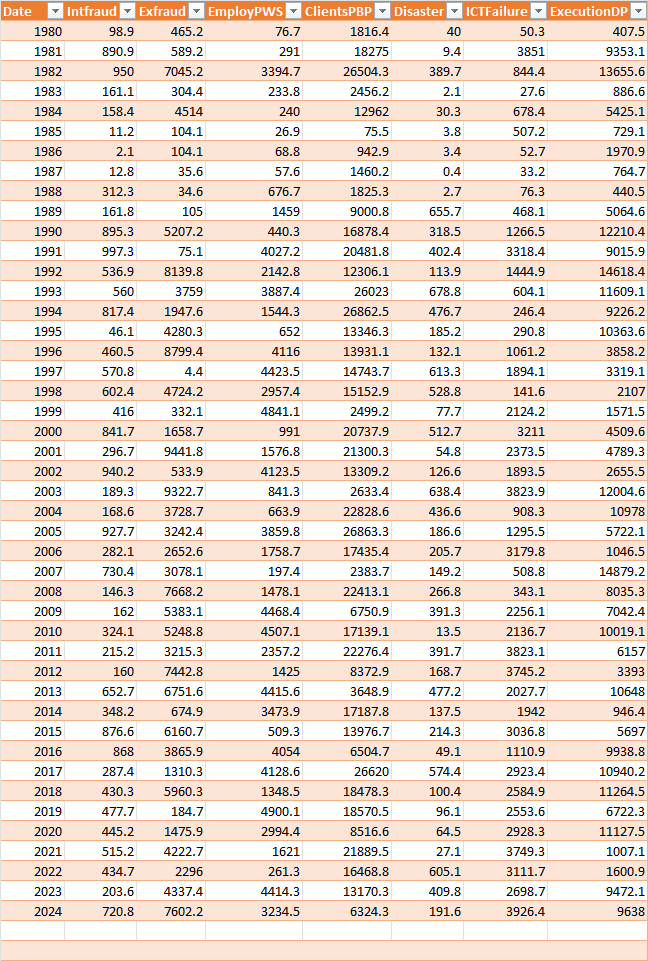
\includegraphics[width=0.75\linewidth]{Summary of the Dataset.png}
    \caption{Operational Risk Loss Data}
    \label{fig: Operational Risk Loss Data}
\end{figure}

\chapter*{Appendix}
\addcontentsline{toc}{chapter}{Appendix}
\section*{Project Code}
\addcontentsline{toc}{section}{Project Code}
\lstinputlisting{bayesian_model_code .py}


\newpage
\begin{figure}[H]
    \centering
    
\includegraphics[width=0.75\linewidth]{Dataset and Github codes.png}
    \caption{Bayesian Belief Network GitHub Codes}
    \label{fig: Dataset and BBN framework Codes}
\end{figure}

 
\end{document}
